\setcounter{section}{3}
\setcounter{subsection}{0}
\setcounter{subsubsection}{0}

% 
\section{Option Keys\\选项键}\label{sec:optkeys}%
\tcbset{external/prefix=external/coreoptions_}
%%%% 使用 \tcbset' 命令设置了一个名为 external/prefix' 的选项,值为 external/coreoptions_'。
%%%% 这个选项用于控制 tcolorbox' 宏包在使用外部化(externalization)功能时生成的文件名前缀。外部化是一种将 tcolorbox' 环境中的内容保存到独立的文件中,并在需要时进行加载的技术,以提高编译速度。通过设置 `external/prefix' 选项,用户可以指定生成的文件名前缀,以便更好地组织和管理外部化的文件。
%%%% 在这个例子中,文件名前缀被设置为 `external/coreoptions_',意味着生成的外部化文件的文件名将以该前缀开始。具体的文件名将由其他参数和命令自动生成。


For the \meta{options} in \refEnvLe{tcolorbox} respectively \refComLe{tcbset}
the following |pgf| keys can be applied. The key tree path |/tcb/| is not to
be used inside these macros. It is easy to add your own style keys using
the syntax for |pgf| keys, see \cite{tantau:tikz_and_pgf,sturm:latex} or the examples
starting from page~\pageref{sec:latextutorial}.

% For the \meta{options} in  respectively 
对于\refEnvLe{tcolorbox}或\refComLe{tcbset}中的\meta{options},可以应用以下|pgf|键。当使用这些命令时,键树路径|/tcb/|是不需要的。%
可以使用|pgf|键的语法轻松添加自己的样式键, 例子见~\pageref{sec:latextutorial}页。%的 \cite{tantau:tikz_and_pgf,sturm:latex} .



% \begin{docTcbKey}{title}{=\meta{text}}{no default, initially empty}
Creates a heading line with \meta{text} as content.

创建以 \meta{text} 作为内容的标题行。

\begin{exdispExample*}{title}{sbs,lefthand ratio=0.6}
\begin{tcolorbox}[title=我的标题行]
这是一个\textbf{tcolorbox}。
\end{tcolorbox}
\end{exdispExample*}
\end{docTcbKey}

\begin{docTcbKey}{notitle}{}{no value, initially set}
Removes the title line if set before.

移除之前设置的标题行。
\end{docTcbKey}

\begin{docTcbKey}{adjusted title}{=\meta{text}}{style, no default, initially unset, 标题高度等高}
Creates a heading line with \meta{text} as content. The minimal height of
this line is adjusted to fit the text given by \refKey{/tcb/adjust text}.
This option makes sense
for single line headings if boxes are set side by side with equal height.
Note that it is very easy to trick this adjustment.


% 创建一个以 \meta{text} 为内容的标题行。 此行的最小高度根据 \meta{text} 自适应。
% 此选项适用于希望让单行放置多个并排的盒子拥有相同的标题高度。
% 注意,to trick 此调整是非常容易的。

创建一个标题行,其中内容为\meta{text}。此行的最小高度会根据\refKey{/tcb/adjust text}中给定的文本进行调整。如果希望让单行放置多个并排的盒子拥有相同的标题高度,则此选项很有意义。请注意,很容易欺骗此调整。
% 诀窍
% 技巧
% 骗局
% 魔术
% 神奇手法
% 欺骗
% 诡计
% 奥妙
% 狡猾手段
% 玩意儿

% exdispExample 
% 这是一个tcolorbox宏包提供的环境,用于生成一个例子展示。runs=2表示该例子最多运行2次,{adjusted_title}是该例子的标题。
\begin{exdispExample}[runs=2]{adjusted_title}
\tcbset{colback=White,arc=0mm,width=(\linewidth-4pt)/4,
equal height group=AT,before=,after=\hfill,fonttitle=\bfseries}

以下标题是not adjusted:\\
\foreach \n in {xxx,ggg,AAA,\"Agypten}
{\begin{tcolorbox}[title=\n,colframe=red!75!black]
一些文本。\end{tcolorbox}}
现在,我们再次尝试adjusted titles:\\
\foreach \n in {xxx,ggg,AAA,\"Agypten}
{\begin{tcolorbox}[adjusted title=\n,colframe=blue!75!black]
一些文本。\end{tcolorbox}}
\end{exdispExample}
\end{docTcbKey}

% todo 
% \tcbset{colback=White,arc=0mm,width=(\linewidth-4pt)/4,equal height group=AT,before=,after=\hfill,fonttitle=\bfseries}:
%这是tcolorbox宏包提供的一个设置环境,可以设置后面生成的tcolorbox的一些属性。
%其中,colback表示背景颜色,arc表示圆角半径,width表示盒子的宽度,
%equal height group表示将多个盒子的高度设置成相同,before和after表示在盒子前后分别添加一些内容,fonttitle表示标题的字体。

% \foreach \n in {xxx,ggg,AAA,\"Agypten}:
% 这是一个foreach循环,用于循环生成tcolorbox盒子。\n表示循环变量,{xxx,ggg,AAA,\"Agypten}是一个包含了4个元素的列表。
% \begin{tcolorbox}[title=\n,colframe=red!75!black]一些文本。\end{tcolorbox}:这是一个tcolorbox环境,用于生成一个盒子。
%title表示盒子的标题,colframe表示边框颜色,一些文本。是盒子中的内容。

% \begin{tcolorbox}[adjusted title=\n,colframe=blue!75!black]一些文本。\end{tcolorbox}:这是一个tcolorbox环境,用于生成一个盒子。
%adjusted title表示盒子的标题,colframe表示边框颜色,一些文本。是盒子中的内容。




\begin{docTcbKey}{adjust text}{=\meta{text}}{no default, initially \texttt{\"Apgjy}}
This sets the reference text for \refKey{/tcb/adjusted title}. If your texts
never exceed \enquote{\"Apgjy} in depth and height you don't need to care about this option.

用于为\refKey{/tcb/adjusted title}设置参考文本。%
如果你的文本不会超过\enquote{\"Apgjy}的深度和高度,你就不需要关心这个选项。

%%%TODO 弄些例子出来看到底啥意思 
% \begin{exdispExample}[runs=2]{adjust_text}
%   \foreach \n in {xxx,ggg,AAA,\"Agypten}
%   {\begin{tcolorbox}[adjust text=\n,title=test,colframe=blue!75!black,width=(\linewidth-4pt)/4]
%   一些文本。\end{tcolorbox}}
% \end{exdispExample}

\end{docTcbKey}

%squeezed 挤压
\begin{docTcbKey}[][doc new=2014-11-24]{squeezed title}{=\meta{text}}{style, no default, initially unset,挤压标题,宽度限最大宽}
Creates a single heading line with \meta{text} as content.
If the \meta{text} is longer than the available space, the text is
squeezed to fit into the available space.

创建一个标题行,内容为 \meta{text}。%
如果 \meta{text} 比可用空间长, 文本将被压缩以适应可用的空间。
\begin{exdispExample}{squeezed_title}
% \tcbuselibrary{raster}
\begin{tcbitemize}[
raster columns=3,%三列
raster equal height,%等高
colframe=red!75!black,colback=red!5!white,%框与背景色
fonttitle=\bfseries%标题加格式
]
\tcbitem[squeezed title={短标题}]
第一个例子
\tcbitem[squeezed title={这是一个非常非常长的标题}]
第二个例子
\tcbitem[squeezed title={这个标题显然对这个例子来说太长了}]
第三个例子
\end{tcbitemize}
\end{exdispExample}
\end{docTcbKey}

% 这是一个使用tcolorbox宏包的例子,展示了如何使用tcbitemize环境创建一个三列等高的项目列表,并对项目的标题进行压缩。
% 具体解释如下:
% 首先加载tcolorbox宏包的raster库,以便使用raster columns和raster equal height选项。

% 然后创建一个tcbitemize环境,并设置raster columns=3和raster equal height选项,以创建一个三列等高的项目列表。

% 接下来,对每个项目使用\tcbitem命令创建一个项目,并使用squeezed title选项压缩项目标题。在本例中,第一个项目的标题为“短标题”,第二个项目的标题为“这是一个非常非常长的标题”,第三个项目的标题为“这个标题显然对这个例子来说太长了”。

% 最后,为了美化效果,设置colframe和colback选项,分别为项目框和背景色添加红色调,并使用fonttitle选项为项目标题添加粗体格式。



%这个 todo 未定义的命令,可能是  tcbitemize 那边才有
% begin{tcolorbox}[squeezed title={BrE əˈdʒʌst, AmE əˈdʒəst},colframe=red!75!black] 
% 一些文本。
% \end{tcolorbox}
% begin{tcolorbox}[squeezed title={BrE skwiːz, AmE skwiz},colframe=red!75!black] 
% 一些文本。
% \end{tcolorbox}
% begin{tcolorbox}[squeezed title={这个标题显然对这个例子来说太长了},colframe=red!75!black] 
% 一些文本。
% \end{tcolorbox}

%试了音标的字体
% \begin{tcbitemize}[
% raster columns=3,%三列
% raster equal height,%等高
% colframe=red!75!black,colback=red!5!white,%框与背景色
% fonttitle=\bfseries%标题加格式
% ]
% \tcbitem[squeezed title={BrE əˈdʒʌst, AmE əˈdʒəst}]
% adjust
% \tcbitem[squeezed title={BrE skwiːz, AmE skwiz}]
% squeeze
% \tcbitem[squeezed title={这个标题显然对这个例子来说太长了}]
% 第三个例子
% \end{tcbitemize}

\begin{docTcbKey}[][doc new=2014-11-24]{squeezed title*}{=\meta{text}}{style, no default, initially unset}
This is a combination of \refKey{/tcb/adjusted title} and  \refKey{/tcb/squeezed title}.

这是  \refKey{/tcb/adjusted title} 和  \refKey{/tcb/squeezed title} 的组合。即高度和宽度都 \dots
\begin{exdispExample}{squeezed_title_2}
% \tcbuselibrary{raster}
\begin{tcbitemize}[raster columns=3,raster equal height,
  colframe=red!75!black,colback=red!5!white,fonttitle=\bfseries]
\tcbitem[squeezed title*={Short title}]
  First box
\tcbitem[squeezed title*={This is a very very long title}]
  Second box
\tcbitem[squeezed title*={This title is clearly to long for this application}]
  Third box
\end{tcbitemize}
\end{exdispExample}
\end{docTcbKey}

\begin{docTcbKey}[][doc new=2019-03-01]{titlebox}{=\meta{mode}}{no default, initially \texttt{visible}}
Controls the treatment of the title part of the box.
Feasible values for \meta{mode} are:

% 控制盒子的标题部分的处理。可设的 \meta{mode} 值有:
控制盒子的标题部分的处理方式。 \meta{mode} 的可行值为:

\begin{DescriptionR}{\docValue{invisible}}
\item[\docValue{visible}]usual type setting of the title box,\\
对带标题盒子的常用的设置,
\item[\docValue{invisible}]empty space instead of the title contents.\\
使用空白代替标题内容。
\end{DescriptionR}

% \begin{DescriptionL}{\docValue{invisible}}
% \item[\docValue{visible}]usual type setting of the title box,\\
% 对带标题盒子的常用的设置,
% \item[\docValue{invisible}]empty space instead of the title contents.\\
% 使用空白代替标题内容。
% \end{DescriptionL}

% \begin{DescriptionLsqueezed}{\docValue{visible}}
% \item[\docValue{visible}]usual type setting of the title box,\\
% 对带标题盒子的常用的设置,
% \item[\docValue{invisible}]empty space instead of the title contents.\\
% 使用空白代替标题内容。
% \end{DescriptionLsqueezed}

% \begin{DescriptionR}{\docValue{invisible}}
% \item[\docValue{visible}]usual type setting of the title box,\\
% 对带标题盒子的常用的设置,
% \item[\docValue{invisible}]empty space instead of the title contents.\\
% 使用空白代替标题内容。
% \end{DescriptionR}

% \begin{description}
% \item[\docValue{visible}]usual type setting of the title box,\\
% 对带标题盒子的常用的设置,
% \item[\docValue{invisible}]empty space instead of the title contents.\\
% 使用空白代替标题内容。
% \end{description}
\begin{exdispExample}{titlebox}
\begin{tcolorbox}[title=我的不可见标题,
  titlebox=invisible]
这是一个\textbf{tcolorbox}.
\end{tcolorbox}
\end{exdispExample}

\begin{exdispExample}{visible_titlebox}
  \begin{tcolorbox}[title=我的可见标题,
    titlebox=visible]
这是一个\textbf{tcolorbox}.
  \end{tcolorbox}
  \end{exdispExample}
\end{docTcbKey}



% \clearpage
\begin{docTcbKey}{detach title}{}{no value}
Detaches the title from its normal position. The text of the title is
stored into \docAuxCommand{tcbtitletext} and the formatted title is
available by \docAuxCommand{tcbtitle}.
The main application is to move the title from its usual place to another one.
  
将标题从它的正常位置移开。标题的文本存储到 \docAuxCommand{tcbtitletext} 中,格式化的标题可以通过 \docAuxCommand{tcbtitle} 获得。主要的应用是将标题从它的惯例位置移动到另一个位置。

% 将标题从其正常位置移开。标题文本存储在\docAuxCommand{tcbtitletext}中,格式化的标题可通过\docAuxCommand{tcbtitle}获得。 主要应用是将标题从其通常位置移动到另一个位置。
 
\begin{exdispExample}{detach_title}
\newtcolorbox{mybox}[2][]{
colbacktitle=red!10!white,
colback=blue!10!white,
coltitle=red!70!black,
title={#2},fonttitle=\bfseries,#1}

\begin{mybox}{My title}
这是一个\textbf{tcolorbox}.
\end{mybox}
\begin{mybox}[detach title,%暂存标题内容到\tcbtitle
before upper={\tcbtitle\quad}%放到upper的前面
]{detach title}
这是一个\textbf{tcolorbox}。\footnotemark
\end{mybox}
\begin{mybox}[detach title,
after upper={\par\hfill\tcbtitle}%放到upper的后面
]{名人名字}
可以用于名人名言的内容。
\end{mybox}
\end{exdispExample}
\end{docTcbKey}
\footnotetext{译者idea:可以改造了当单条的description。}


  

\begin{docTcbKey}{attach title}{}{no value}
  Attaches the title to its normal position. This option is used to reverse
  \refKey{/tcb/detach title}.

  将标题位置重置到其正常位置。此选项用于反转 \refKey{/tcb/detach title}。
  \end{docTcbKey}
  
  
  \begin{docTcbKey}[][doc updated=2015-07-08]{attach title to upper}{\colOpt{=\meta{text}}}{style, default empty, initially unset}
Attaches the title to the begin of the upper part of the box content.
The optional \meta{text} is set between the formatted title and the box content.

将标题附加到框内容upper部分的开头。
可选的 \meta{text} 插入到标题和upper部分内容之间。
  \begin{exdispExample}{attach_title_to_upper}
  \newtcolorbox{mybox}[2][]{colbacktitle=red!10!white,
    colback=blue!10!white,coltitle=red!70!black,
    title={#2},fonttitle=\bfseries,#1}
   
  \begin{mybox}[attach title to upper={\ ---\ }]{My title}
    attach title to upper加值的情况,不仅将标题放到upper之前,还在标题和upper之间放入破折线。
  \end{mybox}
  \begin{mybox}[attach title to upper,after title={:\ }]{My title}
    attach title to upper不加值时,将标题位置放到upper部分之前,再使用after title在标题后加内容。
  \end{mybox}
  \end{exdispExample}
  \end{docTcbKey}



\bigskip
\begin{marker}
More title options are documented in \Vref{subsec:contentadditions}
and \Vref{subsec:skinboxedtitle}.

更多的标题相关配置文档内容见 \Vref{subsec:contentadditions}
和 \Vref{subsec:skinboxedtitle}.
\end{marker}

%【v5 20231025】 2023 0922 %v3 2023-1011      /v4 20231025
% \subsection{Subtitle\\副标题}

Inside the box content, one or more subtitles can be added.
In general, a subtitle is a further \refEnvLe{tcolorbox} which inherits some color and geometry options from the enclosing box. 
It may be customized just like any other \refEnvLe{tcolorbox}.

% 在盒子内,可以添加一个或多个副标题。%
% 一般来说,副标题是一个从封闭盒子继承了一些颜色和几何选项的|tcolorbox|。%
% 它可以像是一个 |tcolorbox| 一样进行设置。  

在盒子内容内部,可以添加一个或多个副标题。 通常,副标题是一个进一步的\refEnvLe{tcolorbox},它从封闭盒子中继承了一些颜色和几何选项。 它可以像任何其他的\refEnvLe{tcolorbox}一样进行自定义。

\begin{docCommand}[doc new=2014-10-10]{tcbsubtitle}{\oarg{options}\marg{text}}
Used inside a \refEnvLe{tcolorbox} to add a subtitle box with the given \meta{text}.
which is formatted by several inherited properties of the enclosing box
by further settings from \refKeyLe{/tcb/subtitle style}, and by the given \meta{options}.

在 \refEnvLe{tcolorbox} 中使用,用于添加一个带有给定 \meta{text} 的副标题框,该框使用封闭框的多个继承属性进行格式设置,并通过 \refKeyLe{/tcb/subtitle style} 的进一步设置和给定的 \meta{options} 进行格式化。

% 在\refEnvLe{tcolorbox}内部,将\meta{text}添加为子标题盒子。
% 这是一个独立的\refEnvLe{tcolorbox},%
% 一些格式从封闭的盒子中继承过来的属性,%
% 也可以通过给\refKeyLe{/tcb/subtitle style}指定的\meta{options}来设定。
\begin{exdispExample*}{tcbsubtitle_1}{%
sbs%是sidebyside的意思
,lefthand ratio=0.6%upper侧占的比例
}
\begin{tcolorbox}[title=我的标题,
colback=red!5!white,
colframe=red!75!black,
fonttitle=\bfseries]
  This is a \textbf{tcolorbox}.
\tcbsubtitle[before skip=\baselineskip]%
  {我的{\tt 副}标题}
进一步的文本。
\end{tcolorbox}
\end{exdispExample*}

% 这段代码使用了tcolorbox宏包,创建了一个带有标题和副标题的盒子。具体解释如下:
% \begin{exdispExample*}{tcbsubtitle_1}{% sbs%是sidebyside的意思 ,lefthand ratio=0.6%upper侧占的比例 }

% 这部分代码是使用exdispExample环境来显示代码和输出结果的,其中使用了sbs选项表示将代码和输出结果并排显示,使用lefthand ratio选项表示代码窗口占整个窗口的比例为0.6。

% \begin{tcolorbox}[title=我的标题, colback=red!5!white, colframe=red!75!black, fonttitle=\bfseries]

% 这部分代码创建了一个tcolorbox盒子,其中包含了一个标题“我的标题”。colback选项表示背景色为红色和白色混合,colframe选项表示边框颜色为红色和黑色混合,fonttitle选项表示标题的字体为粗体。

% This is a \textbf{tcolorbox}.

% 这部分代码在盒子中插入了一段文本“This is a tcolorbox”,其中\textbf命令让“tcolorbox”加粗。

% \tcbsubtitle[before skip=\baselineskip]% {我的{\tt 副}标题}

% 这部分代码创建了一个副标题“我的副标题”,使用了\tcbsubtitle命令。before skip选项表示副标题前面的垂直距离为一个基准行距(\baselineskip),{\tt 副}使用了typewriter字体。

% 进一步的文本。

% 这部分代码在盒子中插入了进一步的文本。

% \end{tcolorbox}

% 这部分代码表示tcolorbox盒子的结束。

\begin{exdispExample*}{tcbsubtitle_2}{sbs,lefthand ratio=0.6}
\begin{tcolorbox}[title=My title,
    colback=red!5!white,
    colframe=red!75!black,
    colbacktitle=yellow!50!red,
    coltitle=red!25!black,
    fonttitle=\bfseries]
  This is a \textbf{tcolorbox}.
\tcbsubtitle[before skip=\baselineskip]%
{我的{\tt 副}标题}
进一步的文本。
\end{tcolorbox}
\end{exdispExample*}
\end{docCommand}

\begin{docTcbKey}[][doc new=2014-10-10]{subtitle style}{=\meta{options}}{no default, initially empty}
Adds |tcolorbox| \meta{options} to the settings for \refCom{tcbsubtitle}.

向 |tcbsubtitle| 设置的副标题的 |tcolorbox| 的 \meta{options} 中设置选项。

\begin{exdispExample*}{subtitle_style}{sbs,lefthand ratio=0.6}
\begin{tcolorbox}[title=My title,
  colback=red!5!white,
  colframe=red!75!black,
  colbacktitle=yellow!50!red,
  coltitle=red!25!black,
  fonttitle=\bfseries,
  subtitle style={boxrule=0.4pt,
    colback=yellow!50!red!25!white} ]
  This is a \textbf{tcolorbox}.
\tcbsubtitle{我的子标题}
  Further text.
\tcbsubtitle[colback=green!50!red!25!white]%
{第二个子标题}
上面的子标题中的背景色覆盖了 |subtitle style| 的设置。
\end{tcolorbox}
\end{exdispExample*}
\end{docTcbKey}
%副标题【v5 20231025 添加了定义】     %v3 2023-1011    /v4 20231025
% \setcounter{section}{4}
\setcounter{subsection}{2}
\setcounter{subsubsection}{0}
\subsection{Upper Part\\upper部分} 

The text content of a \refEnvLe{tcolorbox} may be parted into a mandatory \emph{upper part}
and an optional \emph{lower part}. These parts are separated by
\refComLe{tcblower}. If there is no \refComLe{tcblower} present, there is no
\emph{lower part} and the \emph{upper part} forms the complete text content.

% \refEnvLe{tcolorbox}中的文本内容被分为 \emph{upper 部分} 和一个可选的 \emph{lower 部分}。这两部分由命令 \refComLe{tcblower}分隔。如果没出现 \refComLe{tcblower} ,那么就没有 \emph{lower 部分},\emph{upper 部分}就是所有的内容。

\refEnvLe{tcolorbox} 的文本内容可以分为一个必需的\emph{upper部分}和一个可选的\emph{lower部分}。这些部分由\refComLe{tcblower}分隔。如果没有\refComLe{tcblower},则没有\emph{lower部分},而\emph{upper部分}构成完整的文本内容。

\begin{docTcbKey}[][doc new=2015-01-06]{upperbox}{=\meta{mode}}{no default, initially \texttt{visible}}
Controls the treatment of the upper part of the box. If there is no lower part,  this is the complete text content.
Feasible values for \meta{mode} are:

控制例子的upper部分的显示处理。如果没有lower部分, upper部分内容即是所有内容。
可设置的 \meta{mode} 值有:
\begin{DescriptionL}{\docValue{invisible}}
\item[\docValue{visible}]usual type setting of the upper part,
\par 可见,upper部分的常用设定
\item[\docValue{invisible}] empty space instead of the upper part contents.
\par 不可见,upper部分内容显示为空白。
\end{DescriptionL}
% \begin{exdispExample}{upperbox}
% \begin{tcolorbox}[upperbox=invisible,colback=white%
% ,title=upperbox设置为invisible且没有lower部分]
% 这是一个\textbf{tcolorbox}(但是是隐形的)。
% \end{tcolorbox}

% \begin{tcolorbox}[upperbox=invisible,colback=white%
% ,title=upperbox设置为invisible时只显示lower部分]
% 这是一个\textbf{tcolorbox}(但是是隐形的)。
% \tcblower
% 这是lower部分。
% \end{tcolorbox}
% \end{exdispExample}

\begin{dispExample*}{sbs}
\begin{tcolorbox}[upperbox=invisible%
,colback=white%
,title=upperbox设置为invisible%
且没有lower部分]
这是一个\textbf{tcolorbox}(但是是隐形的)。
\end{tcolorbox}
\end{dispExample*}

\begin{dispExample*}{sbs}
\begin{tcolorbox}[upperbox=invisible%
,colback=white%
,title=upperbox设置为invisible%
时只显示lower部分]
这是一个\textbf{tcolorbox}(但是是隐形的)。
\tcblower
这是lower部分。
\end{tcolorbox}
\end{dispExample*}
 
\end{docTcbKey}


\begin{docTcbKey}[][doc new and updated={2015-01-06}{2019-03-01}]{visible}{}{style, no value}
Shortcut for setting \refKeyLe{/tcb/upperbox}, \refKeyLe{/tcb/lowerbox}, and \refKeyLe{/tcb/titlebox}
to be \docValue{visible}.

同时设置 \refKeyLe{/tcb/upperbox}, \refKeyLe{/tcb/lowerbox}, 和 \refKeyLe{/tcb/titlebox} 为 \docValue{visible} 的快捷方式。
\end{docTcbKey}

\begin{docTcbKey}[][doc new and updated={2015-01-06}{2019-03-01}]{invisible}{}{style, no value}
Shortcut for setting \refKeyLe{/tcb/upperbox}, \refKeyLe{/tcb/lowerbox}, and \refKeyLe{/tcb/titlebox}
to be \docValue{invisible}.

设置 \refKeyLe{/tcb/upperbox}, \refKeyLe{/tcb/lowerbox}, 和 \refKeyLe{/tcb/titlebox} 为 \docValue{invisible} 的快捷方式。
\begin{exdispExample}{invisible}
\begin{tcolorbox}[invisible]
这是一个\textbf{tcolorbox}(但是是隐形的)。
\tcblower
这是\textbf{lower部分}(但是是隐形的)。
\end{tcolorbox}
\end{exdispExample}
\end{docTcbKey}




% \clearpage
\begin{docTcbKey}[][doc new=2015-05-04]{saveto}{=\meta{file name}}{no default, initially empty}
Saves the content of the box into a file for an optional later usage.
This is the counterpart of \refKeyLe{/tcb/savelowerto}, but is saves not
only the upper part but the whole content. If a lower part is present,
it is also saved including \refComLe{tcblower}.

% 将盒子的内容保存到一个文件中,以供以后使用。
% 这和 \refKeyLe{/tcb/savelowerto} 类似, 但它不仅保存了upper部分,是保存了整个内容。
% 如果存在lower部分,也会保存且包含 \refComLe{tcblower}。

将盒子的内容保存到文件中,以备将来需要时使用。这是\refKeyLe{/tcb/savelowerto}的对应项,但不仅保存upper部分,而是保存整个内容。如果存在lower部分,则也会保存,包括\refComLe{tcblower}。

\begin{marker}
This option cannot be combined with \refKeyLe{/tcb/savelowerto}.

此项不能同 \refKeyLe{/tcb/savelowerto} 组合使用.
\end{marker}

\begin{exdispExample}{saveto_1}
\begin{tcolorbox}[invisible%upper、lower都不显示
,saveto=\jobname_mysave1.tex
,colback=white
,before upper={before upper}]
这是一个\textbf{tcolorbox},使用invisible后,看着是空的。
它的内容被saveto暂存到指定的文件中,后续再在其他位置包含进来使用。
\end{tcolorbox}

现在,我们包含进来保存好的文本内容:\\
\input{\jobname_mysave1.tex}


\end{exdispExample}

% before upper

\begin{引述之言}{virhuiai}
在LaTeX中,\verb|\jobname| 代表当前文档的名称(不含扩展名)。
\end{引述之言}

\begin{引述之言}{virhuiai}
如果有\verb|before upper|,但设置了invisible,这部分内容不会写入saveto指定的文件中哦!
\end{引述之言}

% \begin{tcolorbox}[%invisible%upper、lower都不显示
% ,colback=white
% ,before upper={before upper}]
% 这是一个\textbf{tcolorbox},使用invisible后,看着是空的。
% 它的内容被saveto暂存到指定的文件中,后续再在其他位置包含进来使用。
% \end{tcolorbox}

% 在LaTeX中,\jobname代表当前文档的名称(不含扩展名):

% \jobname会展开为去除文件扩展名后的文档名称。

% 例如源文件名为paper.tex,\jobname会展开为paper。

% 如果文件名包含路径,也会去掉路径部分。

% \jobname不包含空格及特殊字符,全部转为小写字母。

% \jobname根据TeX引擎和运行方式有细微差异:

% tex命令默认为文件名。

% latex命令默认为文件名。

% xelatex默认为不含扩展名的文件名。

% \jobname通常用于生成与文档相关的外部文件。

% 也可在导言区重新定义\jobname的值。

% \jobname在标题、摘要、目录等地方也有应用。

% 综上,\jobname可以动态获取文档的名称,对文档编译和内容引用非常有用。它可以确保输出文件名与源文件同步更新。

\begin{exdispExample}{saveto_2}
\begin{tcolorbox}[saveto=\jobname_mysave2.tex]
这是一个\textbf{tcolorbox}.
\tcblower
这是lower部分。
\end{tcolorbox}

现在,我们包含进来保存好的文本内容:
\begin{tcolorbox}[colframe=red,colback=red!10,
coltitle=black,colbacktitle=red!20
,sidebyside%从上下改为左右
,title=在这里我们看到保存的内容包括lower部分]
\input{\jobname_mysave2.tex}
\end{tcolorbox}
\end{exdispExample}
\end{docTcbKey}

% 可以看下这个 mysave2.tex 文件,内容是:

% 这是一个\textbf{tcolorbox}.
% \tcblower
% 这是lower部分。
% 2023 0922   %v3 2023-1011 /v4 20231025
% \begin{docTcbKey}{lowerbox}{=\meta{mode}}{no default, initially \texttt{visible}}
Controls the treatment of the lower part of the box.
Feasible values for \meta{mode} are:

控制lower部分的显示情况。可选的 \meta{mode} 值有:
\begin{DescriptionL}{\docValue{invisible}}
\item[\docValue{visible}]usual type setting of the lower part,
\\可见,lower部分的常用设定

\item[\docValue{invisible}]empty space instead of the lower part contents,
\\不可见,lower部分内容显示为空白。

\item[\docValue{ignored}]the lower part is not used (here).
\\忽略,下部分在这儿没有用上。
\end{DescriptionL}

The last two values are usually applied in connection with |savelowerto|.

后两个选项值通常用于与 |savelowerto| 配合使用。

\begin{exdispExample}{lowerbox}
\begin{tcolorbox}[lowerbox=invisible,colback=white]
This is a \textbf{tcolorbox}.
\tcblower
这是lower部分(但不可见)
\end{tcolorbox}

\begin{tcolorbox}[lowerbox=ignored,colback=white]
This is a \textbf{tcolorbox}.
\tcblower
这是lower部分(但ignored)
\end{tcolorbox}
\end{exdispExample}
\end{docTcbKey}


\begin{docTcbKey}[][doc updated=2014-11-28]{savelowerto}{=\meta{file name}}{no default, initially empty}
Saves the content of the lower part into a file for an optional later usage.

将lower部分的内容保存到一个文件中,以备以后使用。
\begin{exdispExample}{savelowerto}
\begin{tcolorbox}[lowerbox=invisible,savelowerto=\jobname_bspsave.tex,colback=white]
This is a \textbf{tcolorbox}.
\tcblower
这是可能相当复杂的lower部分:
$\displaystyle f(x)=\frac{1+x^2}{1-x^2}$.
\end{tcolorbox}

现在,我们加载保存的文本:\\
\input{\jobname_bspsave.tex}
\end{exdispExample}
\end{docTcbKey}



% \clearpage
\begin{docTcbKey}{lower separated}{\colOpt{=true\textbar false}}{default |true|, initially |true|}
If set to |true|, the lower part is visually separated from the upper part.
It depends on the chosen skin how the visualization of the separation is done.

如果设置为 |true|则lower部分与upper部分可见的分隔开来。
分隔的样式依赖于皮肤的选择。
\enlargethispage*{1cm}
\begin{exdispExample}{lower_separated}
% \tcbuselibrary{skins,raster}
\begin{tcbraster}[colback=red!5!white,colframe=red!75!black,
fonttitle=\bfseries,fontlower=\itshape]
%
\begin{tcolorbox}[title=Lower separated]
This is the upper part.
\tcblower
This is the lower part.
\end{tcolorbox}
%
\begin{tcolorbox}[title=Lower not separated,lower separated=false]
这是upper部分。

设置 |lower separated=false|
\tcblower
这是lower部分。两部分的分隔没有线条出现。
\end{tcolorbox}
%
\begin{tcolorbox}[sidebyside,title=Lower separated]
% 这是upper部分。
|sidebyside|
\tcblower
% 这是lower部分。
两部分变成左右分隔了。
\end{tcolorbox}
%
\begin{tcolorbox}[sidebyside,title=Lower not separated,lower separated=false]
This is the upper part.
\tcblower
This is the lower part.
\end{tcolorbox}
%
\begin{tcolorbox}[beamer,title=Lower separated]
% This is the upper part.
|beamer|
\tcblower
This is the lower part.
\end{tcolorbox}
%
\begin{tcolorbox}[beamer,title=Lower not separated,lower separated=false]
This is the upper part.
\tcblower
This is the lower part.
\end{tcolorbox}
%
\end{tcbraster}
\end{exdispExample}
\end{docTcbKey}




% delimiter
% 定界符
% \clearpage
\begin{docTcbKey}{savedelimiter}{=\meta{name}}{no default, initially \texttt{tcolorbox}}
Used in connection with new environment definitions which extend
|tcolorbox| and use or allow the option |savelowerto|.
To catch the end of the new box environment \meta{name} has to be the name of
this environment. Additionally, the environment definition has to use
|\tcolorbox| instead of
|\begin{tcolorbox}| and |\endtcolorbox| instead of |\end{tcolorbox}|.

% 用于关联由 |newenvironment| 自定义的,拓展自 |tcolorbox| 的新环境中的 |savelowerto| 选项。%
% 要捕获新的盒子环境 \meta{name} 的结尾,必须是这个环境的名字。%
% 此外,环境定义必须使用 |\tcolorbox| 代替 |\begin{tcolorbox}|、用 |\endtcolorbox| 代替 |\end{tcolorbox}|。

用于与扩展了|tcolorbox|并使用或允许选项|savelowerto|的新环境定义相关联。为了捕捉新框环境的结尾,\meta{name}必须是此环境的名称。此外,环境定义必须使用|\tcolorbox|而不是|\begin{tcolorbox}|,并且使用|\endtcolorbox|而不是|\end{tcolorbox}|。

\begin{exdispExample}{savedelimiter1}
\newenvironment{mybox}[1]{%
\tcolorbox[savedelimiter=mybox,
            savelowerto=\jobname_bspsave2.tex,lowerbox=ignored,
            colback=red!5!white,colframe=red!75!black,fonttitle=\bfseries,
            title={#1}]}%
{\endtcolorbox}

\begin{mybox}{暂存 savelowerto 的内容的新环境}
Upper部分。
\tcblower
暂存的lower部分!
\end{mybox}

现在,使用之前暂存的部分:
\begin{tcolorbox}[colback=green!5,title=用到 savelowerto 暂存的内容]
\input{\jobname_bspsave2.tex}
\end{tcolorbox}
\end{exdispExample}

\enlargethispage*{1cm}

The |savedelimiter| is used implicitely with \refCom{newtcolorbox} which
allows a more convenient usage:

上面的 |savedelimiter| 隐式使用了 \refCom{newtcolorbox},和下面对比,使用起来更方便:
\begin{exdispExample}{savedelimiter2}
\newtcolorbox{mybox}[1]{%
            savelowerto=\jobname_bspsave2.tex,lowerbox=ignored,
            colback=red!5!white,colframe=red!75!black,fonttitle=\bfseries,
            title={#1}}%

\begin{mybox}{My Example}
Upper part.
\tcblower
Saved lower part!
\end{mybox}

Now, the saved part is used:
\begin{tcolorbox}[colback=green!5]
\input{\jobname_bspsave2.tex}
\end{tcolorbox}
\end{exdispExample}
\end{docTcbKey}% 2023 0922 %v3 2023-1011   /v4 20231025
% \subsection{Colors and Fonts\\颜色和字体}

\begin{docTcbKey}{colframe}{=\meta{color}}{no default, initially \texttt{black!75!white}}
Sets the frame \meta{color} of the box.

% \hspace{-0.35ex}
设置盒子边框的\meta{color}。
\begin{exdispExample*}{colframe}{sbs,lefthand ratio=0.6}
\begin{tcolorbox}[colframe=red!50!white]
This is a \textbf{tcolorbox}.
\end{tcolorbox}
\end{exdispExample*}
\end{docTcbKey}

\begin{docTcbKey}{colback}{=\meta{color}}{no default, initially \texttt{black!5!white}}
Sets the background \meta{color} of the box.

设置盒子的背景\meta{color}。
\begin{exdispExample*}{colback}{sbs,lefthand ratio=0.6}
\begin{tcolorbox}[colback=red!50!white]
This is a \textbf{tcolorbox}.
\end{tcolorbox}
\end{exdispExample*}
\end{docTcbKey}

另见 \mylib{skins} 库的 \refKeyLe{/tcb/colbacklower}。

\begin{docTcbKey}{title filled}{\colOpt{=true\textbar false}}{default |true|, initially |false|}
Switches the drawing of the title background according to the given value.
This option is set to |true| automatically by \refKeyLe{/tcb/colbacktitle},
\refKeyLe{/tcb/opacitybacktitle}, and \refKeyLe{/tcb/title style},
and \refKeyLe{/tcb/title code}.

根据给定的值切换标题部分背景色的绘制。
\refKeyLe{/tcb/colbacktitle},\refKeyLe{/tcb/opacitybacktitle}, \refKeyLe{/tcb/title style},
和 \refKeyLe{/tcb/title code} 设定时,会自动将此选项设置为 |true|。

\begin{exdispExample*}{title_filled}{sbs,lefthand ratio=0.6}
\begin{tcolorbox}[title=My title,title filled]
This is a \textbf{tcolorbox}.
\end{tcolorbox}
\begin{tcolorbox}[title=My title,
title filled=false]
This is a \textbf{tcolorbox}.
\end{tcolorbox}
\end{exdispExample*}
\end{docTcbKey}


\begin{docTcbKey}{colbacktitle}{=\meta{color}}{no default, initially \texttt{black!50!white}}
Sets the background \meta{color} of the title area of the box.

设置盒子的的标题区域的背景颜色。
\begin{exdispExample*}{colbacktitle}{sbs,lefthand ratio=0.6}
\begin{tcolorbox}[colbacktitle=red!50!white,
title=My title,coltitle=black,
fonttitle=\bfseries]
This is a \textbf{tcolorbox}.
\end{tcolorbox}
\end{exdispExample*}
\end{docTcbKey}



% \clearpage

\begin{docTcbKey}{colupper}{=\meta{color}}{no default, initially \texttt{black}}
Sets the text \meta{color} of the upper part.

设置upper部分的文本的颜色。
\begin{exdispExample*}{colupper}{sbs,lefthand ratio=0.6}
\begin{tcolorbox}[colupper=red!75!black]
This is a \textbf{tcolorbox}.
\tcblower
This is the lower part.
\end{tcolorbox}
\end{exdispExample*}
\end{docTcbKey}


\begin{docTcbKey}{collower}{=\meta{color}}{no default, initially \texttt{black}}
Sets the text \meta{color} of the lower part.

设置lower部分的文本的颜色。
\begin{exdispExample*}{collower}{sbs,lefthand ratio=0.6}
\begin{tcolorbox}[collower=red!75!black]
This is a \textbf{tcolorbox}.
\tcblower
This is the lower part.
\end{tcolorbox}
\end{exdispExample*}
\end{docTcbKey}


\begin{docTcbKey}{coltext}{=\meta{color}}{style, no default, initially \texttt{black}}
Sets the text \meta{color} of the box. This is an abbreviation for setting
|colupper| and |collower| to the same value.

设置盒子中文本的颜色。这是同时将 |colupper| 和 |collower| 的值设置为一个颜色。
\begin{exdispExample*}{coltext}{sbs,lefthand ratio=0.6}
\begin{tcolorbox}[coltext=red!75!black]
This is a \textbf{tcolorbox}.
\tcblower
This is the lower part.
\end{tcolorbox}
\end{exdispExample*}
\end{docTcbKey}


\begin{docTcbKey}{coltitle}{=\meta{color}}{no default, initially \texttt{white}}
Sets the title text \meta{color} of the box.

设置标题的文本的颜色。
\begin{exdispExample*}{coltitle}{sbs,lefthand ratio=0.6}
\begin{tcolorbox}[coltitle=red!75!black,
colbacktitle=black!10!white,title=Test]
This is a \textbf{tcolorbox}.
\end{tcolorbox}
\end{exdispExample*}
\end{docTcbKey}





% \clearpage

\begin{docTcbKey}{fontupper}{=\meta{text}}{no default, initially empty}
Sets \meta{text} before the content of the upper part (e.\,g.\ font settings).

附加 \meta{text} 到{\bf 上}部分的内容之前(例如字体设置)。

% 在上部分的内容之前设置\meta{text}(例如字体设置)。
\begin{exdispExample}{fontupper}
\begin{tcolorbox}[fontupper=Hello!~\sffamily]
This is a \textbf{tcolorbox}.
\end{tcolorbox}
\end{exdispExample}
\begin{exdispExample}{fontupper2}
\begin{tcolorbox}[fontupper=Hello!~]
This is a \textbf{tcolorbox}.
\end{tcolorbox}
\end{exdispExample}
\end{docTcbKey}


\begin{docTcbKey}{fontlower}{=\meta{text}}{no default, initially empty}
Sets \meta{text} before the content of the lower part (e.\,g.\ font settings).

附加 \meta{text} 到lower部分的内容之前(e.\,g.\ 字体设置)。
\begin{exdispExample}{fontlower}
\begin{tcolorbox}[fontlower=\sffamily\bfseries]
This is a \textbf{tcolorbox}.
\tcblower
This is the lower part.
\end{tcolorbox}
\end{exdispExample}
\end{docTcbKey}


\begin{docTcbKey}{fonttitle}{=\meta{text}}{no default, initially empty}
Sets \meta{text} before the content of the title text (e.\,g.\ font settings).

附加 \meta{text} 到标题文本的内容之前(e.\,g.\ 字体设置)。
\begin{exdispExample}{fonttitle}
\begin{tcolorbox}[fonttitle=\sffamily\bfseries\large,title=Hello]
This is a \textbf{tcolorbox}.
\end{tcolorbox}
\end{exdispExample}
\begin{exdispExample}{fonttitle2}
\begin{tcolorbox}[fonttitle=只加了文字,title=Hello]
This is a \textbf{tcolorbox}.
\end{tcolorbox}
\end{exdispExample}
\end{docTcbKey}

\bigskip
\begin{marker}
More color options are provided by using skins documented in
Section \ref{sec:skins} from page \pageref{sec:skins}.

更多的颜色选项是通过使用 \pageref{sec:skins} 页第 \ref{sec:skins} 节中介绍的 |skins| 提供的。
\end{marker}%【v5 20231025】  2023 0922 %v3 2023-1011   /v4 20231025
% \setcounter{section}{4}
\setcounter{subsection}{5}
\setcounter{subsubsection}{0}
 
\subsection{Text Alignment文本对齐}
\begin{docTcbKey}[][doc new=2015-05-07]{halign}{=\meta{alignment}}{no default, initially \texttt{justify}}
If there is no lower part, |halign| determines the horizontal \meta{alignment}
of the text content.
Otherwise, |halign| determines the horizontal \meta{alignment}
of the upper part of the box only.
The feasible values for \meta{alignment} are more or less identical to
the corresponding |/tikz/align| settings, even if the implementation differs.

确定盒子upper部分的水平\meta{alignment}方式。可行的\meta{alignment}值与相应的|/tikz/align|设置几乎相同,即使实现不同。\\[1em]

% 如果没有lower部分, |halign| 决定着水平的文本内容的对齐方式为 \meta{alignment}。
% 否则, |halign| 的 \meta{alignment} 只影响到upper部分的水平对齐。
% |halign| 决定着upper部分文本内容的水平对齐方式为 \meta{alignment}。
% \meta{alignment} 可选的值有不少同 |/tikz/align| 的相应设置是一样的, 即使实现有所不同。

\sbox{\cshDocValueLikeItemBox}{\docValue{flush center}}%%% 调用前设置,以用来指定宽度
% \setlength\cshDocValueLikeItemBoxWd{\wd\cshDocValueLikeItemBox}

\cshDocValueAndTwoDescLikeItem{justify}{usual left and right justified type setting.}{常用的,左右对齐%的排版设置(两端对齐)
。}

\cshDocValueAndTwoDescLikeItem{left}{left border justification in analogy to plain \TeX.}{类似于plain \TeX 的左边界对齐。}

\cshDocValueAndTwoDescLikeItem{flush left}
{left border justification with |\raggedright| of \LaTeX.}
{向着盒子的左边框对齐。}%,使用 \LaTeX 的 |\raggedright|\footnote{ragged是不整齐的意思}。

\cshDocValueAndTwoDescLikeItem{right}{right border justification in analogy to plain \TeX.}
{向着盒子的右边框对齐。}%,类似于 plain \TeX。

\cshDocValueAndTwoDescLikeItem{flush right}{right border justification with |\raggedleft| of \LaTeX.}
{向着盒子的右边框对齐。}%使用 \LaTeX 的 |\raggedleft|。

\cshDocValueAndTwoDescLikeItem{center}{centering in analogy to plain \TeX.}
{居中对齐.}%,使用 plain \TeX。

\cshDocValueAndTwoDescLikeItem{flush center}{centering with |\centering| of \LaTeX.}
{居中对齐。}%,使用 \LaTeX 的 |\centering|。


% \begin{DescriptionR}{\docValue{flush center}}
% \item[\docValue{justify}] usual left and right justified type setting.
% \par 常用的,左右对齐%的排版设置(两端对齐)。
% \item[\docValue{left}]left border justification in analogy to plain \TeX.
% \par 类似于plain \TeX 的左边界对齐。
% % 向着盒子的左边框对齐,类似于 plain \TeX。
% \item[\docValue{flush left}]
% left border justification with |\raggedright| of \LaTeX.
% \par 向着盒子的左边框对齐。%,使用 \LaTeX 的 |\raggedright|\footnote{ragged是不整齐的意思}。
% \item[\docValue{right}]right border justification in analogy to plain \TeX.
% \par 向着盒子的右边框对齐。%,类似于 plain \TeX。
% \item[\docValue{flush right}]right border justification with |\raggedleft| of \LaTeX.
% \par 向着盒子的右边框对齐。%使用 \LaTeX 的 |\raggedleft|。
% \item[\docValue{center}]centering in analogy to plain \TeX.
% \par 居中对齐.%,使用 plain \TeX。
% \item[\docValue{flush center}]centering with |\centering| of \LaTeX.
% \par 居中对齐。%,使用 \LaTeX 的 |\centering|。
% \end{DescriptionR}

The differences between the flush and non-flush version are explained in
detail in the \tikzname\ manual \cite{tantau:tikz_and_pgf}. The short story is that
the non-flush versions will often look more balanced but with more
hyphenations.

% 在 \tikzname\ 手册 %\cite{tantau:tikz_and_pgf} 
% 中详细介绍了 flush 和 non-flush 版本之间的区别。简而言之 non-flush 版本通常看起来更加平衡,但是有更多的连字符。

在\tikzname\ 手册\cite{tantau:tikz_and_pgf}中详细解释了flush版本和non-flush版本之间的区别。简短的说,non-flush版本通常看起来更平衡,但会有更多的连字。

% \begin{tcolorbox}[adjusted title=flush center,halign=flush center]
%   This is a demonstration text for showing how line breaking works.
%   \end{tcolorbox}
%   \begin{tcolorbox}[adjusted title=flush left,halign=flush left]
%   This is a demonstration text for showing how line breaking works.
%   \end{tcolorbox}
%   \begin{tcolorbox}[adjusted title=flush right,halign=flush right]
%   This is a demonstration text for showing how line breaking works.
%   \end{tcolorbox}
  
%   \begin{tcolorbox}[adjusted title=center,halign=center]
%   This is a demonstration text for showing how line breaking works.
%   \end{tcolorbox}
%   \begin{tcolorbox}[adjusted title=left,halign=left]
%   This is a demonstration text for showing how line breaking works.
%   \end{tcolorbox}
%   \begin{tcolorbox}[adjusted title=right,halign upper=right]
%   This is a demonstration text for showing how line breaking works.
%   \end{tcolorbox}
  

\begin{exdispExample}{halign}
\tcbset{colback=red!5!white,colframe=red!75!black,size=small,
fonttitle=\bfseries,width=3.5cm,box align=top,
nobeforeafter}

\foreach \p in {flush center,flush left,flush right}
{\begin{tcolorbox}[adjusted title=\p,halign=\p]
This is a demonstration text for showing how line breaking works.
\end{tcolorbox}
}

\foreach \q in {center, left, right}
{\begin{tcolorbox}[adjusted title=\q,halign=\q]
This is a demonstration text for showing how line breaking works.
\end{tcolorbox}
} 

\end{exdispExample}
\end{docTcbKey}

\end{document}

\begin{docTcbKey}[][doc new=2015-05-07]{halign upper}{=\meta{alignment}}{no default, initially \texttt{justify}}
% Alias for \refKeyLe{/tcb/halign}.

\refKeyLe{/tcb/halign} 的别名
\end{docTcbKey}



% \newpage
\begin{docTcbKey}[][doc new=2015-05-07]{halign lower}{=\meta{alignment}}{no default, initially \texttt{justify}}
|halign lower| determines the horizontal \meta{alignment} of the lower part of the box.
The feasible values for \meta{alignment} are the same as for \refKeyLe{/tcb/halign}.

% |halign lower| 控制着盒子的lower部分的内容的水平对齐方式为 \meta{alignment}。\meta{alignment} 的可选值同 \refKeyLe{/tcb/halign} 一样。

|halign lower| 确定盒子lower部分的水平 \meta{alignment}。 \meta{alignment} 的可行值与 \refKeyLe{/tcb/halign} 相同。
\begin{exdispExample}{halign_lower}
\begin{tcbraster}[raster columns=3,fonttitle=\bfseries,
colback=red!5!white,colframe=red!75!black]

\begin{tcolorbox}[adjusted title=flush center,halign lower=flush center]
Upper part. \tcblower Lower part.
\end{tcolorbox}
\begin{tcolorbox}[adjusted title=flush left,halign lower=flush left]
Upper part. \tcblower Lower part.
\end{tcolorbox}
\begin{tcolorbox}[adjusted title=flush right,halign lower=flush right]
Upper part. \tcblower Lower part.
\end{tcolorbox}
\begin{tcolorbox}[adjusted title=center,halign lower=center]
Upper part. \tcblower Lower part.
\end{tcolorbox}
\begin{tcolorbox}[adjusted title=left,halign lower=left]
Upper part. \tcblower Lower part.
\end{tcolorbox}
\begin{tcolorbox}[adjusted title=right,halign lower=right]
Upper part. \tcblower Lower part.
\end{tcolorbox}

\end{tcbraster}
\end{exdispExample}
\end{docTcbKey}






% \clearpage
%这儿原来写错了
\begin{docTcbKey}[][doc new=2022-10-30]{halign title}{=\meta{alignment}}{no default, initially \texttt{justify}}
|halign title| determines the horizontal \meta{alignment} of the title of the box.
The feasible values for \meta{alignment} are the same as for \refKeyLe{/tcb/halign}.

|halign title| 设置盒子的标题部分的对齐方式为 \meta{alignment}。
\meta{alignment} 的可选值同 \refKeyLe{/tcb/halign} 一样。

\begin{exdispExample}{halign_title}
\begin{tcbraster}[raster columns=3,fonttitle=\bfseries,
colback=red!5!white,colframe=red!75!black]

\begin{tcolorbox}[adjusted title=flush center,halign title=flush center]
This is a \textbf{tcolorbox}.
\end{tcolorbox}
\begin{tcolorbox}[adjusted title=flush left,halign title=flush left]
This is a \textbf{tcolorbox}.
\end{tcolorbox}
\begin{tcolorbox}[adjusted title=flush right,halign title=flush right]
This is a \textbf{tcolorbox}.
\end{tcolorbox}
\begin{tcolorbox}[adjusted title=center,halign title=center]
This is a \textbf{tcolorbox}.
\end{tcolorbox}
\begin{tcolorbox}[adjusted title=left,halign title=left]
This is a \textbf{tcolorbox}.
\end{tcolorbox}
\begin{tcolorbox}[adjusted title=right,halign title=right]
This is a \textbf{tcolorbox}.
\end{tcolorbox}

\end{tcbraster}
\end{exdispExample}
\end{docTcbKey}




% \enlargethispage*{1cm}

\begin{docTcbKey}[][doc updated=2015-05-07]{flushleft upper}{}{style, no value}
Shortcut for setting \refKeyLe{/tcb/halign} to \docValue{flush left}.
将 \refKeyLe{/tcb/halign} 设置为 \docValue{flush left} 的简写形式。
\end{docTcbKey}

\begin{docTcbKey}[][doc updated=2015-05-07]{center upper}{}{style, no value}
Shortcut for setting \refKeyLe{/tcb/halign} to \docValue{flush center}.

将 \refKeyLe{/tcb/halign} 设置为 \docValue{flush center} 的简写形式。
\end{docTcbKey}

\begin{docTcbKey}[][doc updated=2015-05-07]{flushright upper}{}{style, no value}
Shortcut for setting \refKeyLe{/tcb/halign} to \docValue{flush right}.

将 \refKeyLe{/tcb/halign} 设置为 \docValue{flush right} 的简写形式。
\end{docTcbKey}

\begin{docTcbKey}[][doc updated=2015-05-07]{flushleft lower}{}{style, no value}
Shortcut for setting \refKeyLe{/tcb/halign lower} to \docValue{flush left}.

将 \refKeyLe{/tcb/halign lower} 设置为 \docValue{flush left} 的简写形式。
\end{docTcbKey}

\begin{docTcbKey}[][doc updated=2015-05-07]{center lower}{}{style, no value}
Shortcut for setting \refKeyLe{/tcb/halign lower} to \docValue{flush center}.
将 \refKeyLe{/tcb/halign lower} 设置为 \docValue{flush center} 的简写形式。
\end{docTcbKey}

\begin{docTcbKey}[][doc updated=2015-05-07]{flushright lower}{}{style, no value}
Shortcut for setting \refKeyLe{/tcb/halign lower} to \docValue{flush right}.

将 \refKeyLe{/tcb/halign lower} 设置为 \docValue{flush right} 的简写形式。
\end{docTcbKey}



% \clearpage

\begin{docTcbKey}[][doc updated=2015-05-07]{flushleft title}{}{style, no value}
Shortcut for setting \refKeyLe{/tcb/halign title} to \docValue{flush left}.

将 \refKeyLe{/tcb/halign title} 设置为 \docValue{flush left} 的简写形式。
\end{docTcbKey}

\begin{docTcbKey}[][doc updated=2015-05-07]{center title}{}{style, no value}
Shortcut for setting \refKeyLe{/tcb/halign title} to \docValue{flush center}.

将 \refKeyLe{/tcb/halign title} 设置主 \docValue{flush center} 的简写形式。
\end{docTcbKey}

\begin{docTcbKey}[][doc updated=2015-05-07]{flushright title}{}{style, no value}
Shortcut for setting \refKeyLe{/tcb/halign title} to \docValue{flush right}.

将 \refKeyLe{/tcb/halign title} 设置为 \docValue{flush right} 的简写形式。
\end{docTcbKey}


\begin{marker}
The vertical alignment settings are only relevant for boxes which are larger
than their natural height, see \Fullref{sec:heightcontrol}.

垂直对齐设置只适用于大于其自然高度的盒子。见 \Fullref{sec:heightcontrol}.
\end{marker}

\begin{docTcbKey}[][doc updated=2015-07-16]{valign}{=\meta{alignment}}{no default, initially |top|}
If the height of a |tcolorbox| is not the natural height, |valign|
determines the vertical \meta{alignment} of the upper part.
Feasible values are

如果一个 |tcolorbox| 的盒子的高度不是其自然高度\footnote{译注:指定了高度}, |valign| 控制着盒子的upper部分的对方方式 \meta{alignment} 。
可选的值有:
\begin{itemize}
\item\docValue{top}: %Anchor text at top.
顶部对齐。
\item\docValue{center}: %Anchor text at center.
中间对齐。
\item\docValue{bottom}:% Anchor text at bottom.
底部对齐。
\item\docValue{scale}: 
Scale text vertically to fit into the available space.
  This is brutal and may not look very good. Consider \Fullref{sec:fitting}
  alternatively.
垂直缩放文本以适应可用空间。
这简单粗暴,可能看起来不是很好。或者考虑下 \Fullref{sec:fitting}。


\item\docValue{scale*}: 
Like \docValue{scale}, but scaling is bounded by
  \refKeyLe{/tcb/valign scale limit}.

类似于\docValue{scale}, 但缩放范围受限于 \refKeyLe{/tcb/valign scale limit}.
\end{itemize}
For a box with natural height, these settings are meaningless.

对于具有自然高度的盒子,这些设置毫无意义。
\begin{exdispExample}{valign}
\tcbset{width=(\linewidth-2mm)/4,before=,after=\hfill,
colframe=blue!75!black,colback=white,height=2cm}

\foreach \myalign in {top,center,bottom,scale}
{\begin{tcolorbox}[valign=\myalign]
This is a \textbf{tcolorbox}.
\end{tcolorbox}}
\end{exdispExample}
\end{docTcbKey}






\begin{docTcbKey}[][doc new=2015-05-07]{valign upper}{=\meta{alignment}}{no default, initially \texttt{top}}
Alias for \refKeyLe{/tcb/valign}.

\refKeyLe{/tcb/valign} 的别名。
\end{docTcbKey}

\begin{docTcbKey}{valign lower}{=\meta{alignment}}{no default, initially |top|}
This key has the same meaning for the lower part as |valign|
for the upper part, i.\,e., it determines
the vertical \meta{alignment} of the lower part with feasible values
|top|, |center|, |bottom|, |scale|, and |scale*|.

此项设置含义同upper部分的 |valign| 相同, i.\,e., 它指定了lower部分的竖直方向的对齐方式 \meta{alignment} ,可选的值有 |top|, |center|, |bottom|, |scale|, 和 |scale*|.

\end{docTcbKey}

\begin{docTcbKey}[][doc new=2015-07-16]{valign scale limit}{=\meta{real number}}{no default, initially \texttt{1.1}}
Sets an upper scale limit for the \docValue{scale*} setting in
\refKeyLe{/tcb/valign} and \refKeyLe{/tcb/valign lower}.
Note that this value is not reset by \refKeyLe{/tcb/reset}. So, changes
also apply to embedded boxes.

设置 \docValue{scale*} 在指定 \refKeyLe{/tcb/valign} 和 \refKeyLe{/tcb/valign lower} 时缩放的范围上限。注意,此值不会随着 \refKeyLe{/tcb/reset} 而重置。所以,修改的话也会同时在嵌套的盒子中生效。
\end{docTcbKey}

Also see \refKeyLe{/tcb/sidebyside align} for alignment settings when
upper part and lower part are set side-by-side.

另见 \refKeyLe{/tcb/sidebyside align} 了解当设置为side-by-side左右排布时的对齐选项。 %}%【v5 20231025 定义了新的命令 cshDocValueLikeItemBox 】v3 2023-1011                /v4 20231025
% \subsection{Geometry\\几何形状}

% \subsubsection{Width} 

\begin{docTcbKey}{width}{=\meta{length}}{no default, initially \cs{linewidth}}
Sets the total width of the colored box to \meta{length}.
See also \refKeyLe{/tcb/height}.

将%有色的带框
盒子的总宽度设置为 \meta{length}。另见 \refKeyLe{/tcb/height}。
\begin{exdispExample}{width} 
\tcbset{colback=red!5!white,colframe=red!75!black}

\begin{tcolorbox}[width=\linewidth/2]
这是一个\textbf{tcolorbox}.
\end{tcolorbox}
\end{exdispExample}
\end{docTcbKey}


\begin{docTcbKey}[][doc new=2014-10-31]{text width}{=\meta{length}}{style, no default}
Sets the text width of the upper part to \meta{length}.
See also \refKeyLe{/tcb/text height}.

将upper部分的文本宽度设置为 \meta{length}.
另见 \refKeyLe{/tcb/text height}.
\begin{exdispExample}{text_width}
\tcbset{colback=red!5!white,colframe=red!75!black}

\begin{tcolorbox}[text width=4cm]
This is a \textbf{tcolorbox} where the text has a width of 4cm.
\end{tcolorbox}
\end{exdispExample}
\end{docTcbKey}

\begin{docTcbKey}[][doc new=2014-11-07]{add to width}{=\meta{length}}{style, no default}
Adds \meta{length} to the current total width of the colored box.

将当前盒子的总宽度增加 \meta{length} 。    
\begin{exdispExample*}{add_to_width}{sbs,lefthand ratio=0.6}
\tcbset{width=4cm,colback=red!5!white,
colframe=red!75!black}

\begin{tcolorbox}
这是一个\textbf{tcolorbox}.
\end{tcolorbox}

\begin{tcolorbox}[add to width=1cm]
这是一个\textbf{tcolorbox}.
\end{tcolorbox}
\end{exdispExample*}
\end{docTcbKey}
See \Fullref{sec:heightcontrol} for setting fixed height values.

有关设置固定高度值的问题,请参阅 \Fullref{sec:heightcontrol}。
% \setcounter{section}{4}
% \setcounter{subsection}{7}
% \setcounter{subsubsection}{1}
% \subsubsection{Rules\\线}
\begin{docTcbKey}{toprule}{=\meta{length}}{no default, initially \texttt{0.5mm}}
Sets the line width of the top rule to \meta{length}.

设置顶边框线的宽度为 \meta{length}。
\begin{exdispExample}{toprule}
\tcbset{colback=red!5!white,colframe=red!75!black}

\begin{tcolorbox}[toprule=3mm]
这是一个\textbf{tcolorbox}.
\end{tcolorbox}
\end{exdispExample}
\end{docTcbKey}


\begin{docTcbKey}{bottomrule}{=\meta{length}}{no default, initially \texttt{0.5mm}}
Sets the line width of the bottom rule to \meta{length}.

设置底边框线的宽度为 \meta{length}。
\begin{exdispExample}{bottomrule}
\tcbset{colback=red!5!white,colframe=red!75!black}

\begin{tcolorbox}[bottomrule=3mm]
这是一个\textbf{tcolorbox}.
\end{tcolorbox}
\end{exdispExample}
\end{docTcbKey}

\begin{docTcbKey}{leftrule}{=\meta{length}}{no default, initially \texttt{0.5mm}}
Sets the line width of the left rule to \meta{length}.

设置左边框线的宽度为 \meta{length}。
\begin{exdispExample}{leftrule}
\tcbset{colback=red!5!white,colframe=red!75!black}

\begin{tcolorbox}[leftrule=3mm]
这是一个\textbf{tcolorbox}.
\end{tcolorbox}
\end{exdispExample}
\end{docTcbKey}


\begin{docTcbKey}{rightrule}{=\meta{length}}{no default, initially \texttt{0.5mm}}
Sets the line width of the right rule to \meta{length}.

设置右边框线的宽度为 \meta{length}。
\begin{exdispExample}{rightrule}
\tcbset{colback=red!5!white,colframe=red!75!black}

\begin{tcolorbox}[rightrule=3mm]
这是一个\textbf{tcolorbox}.
\end{tcolorbox}
\end{exdispExample}
\end{docTcbKey}




% \clearpage
\begin{docTcbKey}{titlerule}{=\meta{length}}{no default, initially \texttt{0.5mm}}
Sets the line width of the rule below the title to \meta{length}.

设置标题文本下方的线的宽度为 \meta{length}。
\begin{exdispExample}{titlerule}
\tcbset{enhanced,colback=red!5!white,colframe=red!75!black,
colbacktitle=red!90!black}

\begin{tcolorbox}[titlerule=3mm,title=This is the title]
这是一个\textbf{tcolorbox}.
\end{tcolorbox}
\end{exdispExample}
\end{docTcbKey}


\begin{docTcbKey}{boxrule}{=\meta{length}}{style, no default, initially \texttt{0.5mm}}
Sets all rules of the frame to \meta{length}, i.\,e.\ 
\refKeyLe{/tcb/toprule}, \refKeyLe{/tcb/bottomrule}, \refKeyLe{/tcb/leftrule},
\refKeyLe{/tcb/rightrule}, and \refKeyLe{/tcb/titlerule}.

设置所有的边框线的宽度为 \meta{length}\footnote{i.\,e.\ 
\refKeyLe{/tcb/toprule}, \refKeyLe{/tcb/bottomrule}, \refKeyLe{/tcb/leftrule},
\refKeyLe{/tcb/rightrule}, 和 \refKeyLe{/tcb/titlerule}.}。
\begin{exdispExample}{boxrule}
\tcbset{colback=red!5!white,colframe=red!75!black}

\begin{tcolorbox}[boxrule=3mm]
这是一个\textbf{tcolorbox}.
\end{tcolorbox}
\end{exdispExample}
\end{docTcbKey}

\bigskip
\begin{marker}
More options for drawing a \refKeyLe{/tcb/borderline} are provided by using skins documented in
Section \ref{sec:skins} from page \pageref{sec:skins}.

更多的关于绘制 \refKeyLe{/tcb/borderline} 的选项的描述在 skins 的文档中,详见 \pageref{sec:skins} 页的 \ref{sec:skins} 小节。
\end{marker}


% \setcounter{section}{4}
% \setcounter{subsection}{7}
% \setcounter{subsubsection}{2}
% % Arcs\hfill 
\subsubsection{弧线}
\begin{docTcbKey}{arc}{=\meta{length}}{no default, initially \texttt{1mm}}
Sets the inner radius of the four frame arcs to \meta{length}.

设置边框的四个角落的弧的内半径为 \meta{length}。

% \begin{exdispExample}{arc}
% \tcbset{colback=red!5!white,colframe=red!75!black}
% \begin{tcolorbox}[arc=0mm]
% 这是一个\textbf{tcolorbox}.
% \end{tcolorbox}
% \begin{tcolorbox}[arc=3mm]
% 这是一个\textbf{tcolorbox}.
% \end{tcolorbox}
% \end{exdispExample}

\begin{dispExample*}{sidebyside,lefthand ratio=0.6}
\tcbset{colback=red!5!white,colframe=red!75!black}
\begin{tcolorbox}[arc=0mm]
这是一个\textbf{tcolorbox}.
\end{tcolorbox}
\end{dispExample*}

\begin{dispExample*}{sidebyside,lefthand ratio=0.6}
\tcbset{colback=red!5!white,colframe=red!75!black}
\begin{tcolorbox}[arc=3mm]
这是一个\textbf{tcolorbox}.
\end{tcolorbox}
\end{dispExample*}
\end{docTcbKey}



% \begin{exdispExample*}{arc_default}{sbs,lefthand ratio=0.6}
 
% \end{exdispExample*}

% \begin{exdispExample*}{arc_3cm}{sbs,lefthand ratio=0.6}
 
% \end{exdispExample*}

% gpt4:
% 在 LaTeX 中,颜色的混合可以使用 ! 符号来实现。这种写法叫做 "interpolation of colors"。

% red!5!white 的意思是,颜色由5%的红色和95%的白色混合而成。结果是一个非常浅的红色。

% red!75!black 的意思是,颜色由75%的红色和25%的黑色混合而成。结果是一个较深的红色。

% claude
% !后面的数字表示混合比例,范围是0到100。
% 0表示完全使用第一个颜色。
% 100表示完全使用第二个颜色。
% 所以:

% red!0!white 等同于纯红色red。
% red!100!white 等同于纯白色white。


% \clearpage
\begin{docTcbKey}[][doc new=2015-05-05]{circular arc}{}{style, no value}
  Sets \refKeyLe{/tcb/arc} to match the half of the inner width of the colored box.
  If width and height of the box are identical, this gives a circle.
  
  将 \refKeyLe{/tcb/arc} 设置为盒子内部宽度的一半。如果盒子的宽度和高度相同,就会得到一个圆。
  \begin{marker}
  If the height of the box is smaller than the width, the result will look
  quite ugly.
  
  如果盒子的高度小于宽度,结果看起来会很难看。   
  \end{marker}
  \begin{exdispExample*}{circular_arc}{sbs,lefthand ratio=0.6}
  \begin{tcolorbox}[width=3cm,
  colback=red!5!white,
  colframe=red!75!black,
  halign=center,valign=center,
  square,circular arc]
  这是一个\textbf{tcolorbox}.
  \end{tcolorbox}
  \end{exdispExample*}
  \end{docTcbKey}
  
  
  \begin{docTcbKey}[][doc new=2015-05-05]{bean arc}{}{style, no value}
  Sets \refKeyLe{/tcb/arc} to match the smaller value of the
  half of the inner width and of the inner height of the colored box.
  
%   设置 \refKeyLe{/tcb/arc} 为盒子内宽和内高中较小者值的一半。
  
  将\refKeyLe{/tcb/arc}设置为盒子内宽度一半和高度一半的较小值。

  \begin{marker}
  This only works for a fixed \refKeyLe{/tcb/height}. Also, \refKeyLe{/tcb/bean arc}
  must be used \emph{after} width and height are set by option keys.
  
%   这只适用于 \refKeyLe{/tcb/height} 为固定值的情况。此外,\refKeyLe{/tcb/bean arc} 选项设置需要在设置宽度和高度之后。
  这仅适用于固定的\refKeyLe{/tcb/height}。另外,\refKeyLe{/tcb/bean arc}必须在宽度和高度由选项键设置之后使用。
  \end{marker}
  \begin{exdispExample*}{bean_arc}{sbs,lefthand ratio=0.6}
  \tcbset{size=fbox,boxrule=0.5mm,
  colback=red!5!white,
  colframe=red!75!black,
  halign=center,valign=center}
  
  \begin{tcolorbox}[width=3cm,height=2cm,
  bean arc]
  Box A
  \end{tcolorbox}
  
  \begin{tcolorbox}[width=2cm,height=3cm,
  bean arc]
  Box B
  \end{tcolorbox}
  \end{exdispExample*}
  \end{docTcbKey}
  
  % 八角形
  \begin{docTcbKey}[][doc new=2015-05-05]{octogon arc}{}{style, no value}
  Sets \refKeyLe{/tcb/arc} to match $\frac{1}{2+\sqrt{2}}$ of the inner width
  of the colored box. If width and height of the box are identical,
  the interior is a regular octogon.

将\refKeyLe{/tcb/arc}设置为盒子的内部宽度的$\frac{1}{2+\sqrt{2}}$。如果盒子的宽度和高度相同,则内部是一个正八边形。

% 设置 \refKeyLe{/tcb/arc} 为盒子内部宽度的 $\frac{1}{2+\sqrt{2}}$ 。如果盒子的宽度和高度相同,内部是一个规则的八边形。
  % \begin{tcolorbox}[
  %   width=2.1cm,octogon arc,
  %   ]
  %   STOP
  %   \end{tcolorbox}
\begin{exdispExample*}{octogon_arc}{sbs,lefthand ratio=0.8}
\begin{tcolorbox}[enhanced,% enhanced: 启用高级选项。
size=minimal,% size=minimal: 去除默认边距,仅显示框体。
auto outer arc,% auto outer arc: 自动调整外部圆角半径以适应框体大小。
width=2.1cm,octogon arc,% octogon arc: 外部圆角为八角形。
colback=red,% colback=red: 背景色为红色。
colframe=white,% colframe=white: 边框颜色为白色。
colupper=white,% colupper=white: 文字颜色为白色。
fontupper=\fontsize{7mm}{7mm}\selectfont\bfseries\sffamily,
%文字大小为7毫米,粗体,无衬线字体。
halign=center,valign=center,
% halign=center: 水平居中对齐。% valign=center: 垂直居中对齐。
square,% square: 边框为直角。
arc is angular,% arc is angular: 内部圆角为直角。
borderline={0.2mm}{-1mm}{red}  ]%使用红色的0.2毫米线条作为边框,内部偏移1毫米。
STOP
\end{tcolorbox}
\end{exdispExample*}
\end{docTcbKey}




  

% angular,有角度的
% \clearpage
\begin{docTcbKey}[][doc new=2015-05-05]{arc is angular}{}{no value, initially unset}
  Using this options applies a patch which straightens the corners arcs of
  the boxes. The little arcs are replaced by little straight lines.
  
%   这个选项\footnote{arc is angular}用于对盒子四角弧线的一个补丁。小弧线被小直线代替。

  使用此选项将应用一个补丁,使盒子的角弧线变直。小弧线将被小直线替换。
  \begin{marker}
  This patch is considered as an experimental feature.
  It changes some of the original \tikzname\ code. This change may break
  with future updates of \tikzname.
  
%   这个补丁被认为是一个实验性的特征。它改变了一些原始的 \tikzname\ 代码。此更改可能会随着 \tikzname\ 的未来更新而中断。
  这个补丁被视为一项实验性的功能。它改变了一些原始的\tikzname 代码。这种改变可能会在未来的\tikzname 更新中出现问题。
  \end{marker}
  
  \begin{exdispExample*}{arc_is_angular}{sbs,lefthand ratio=0.6}
  \tcbset{colback=red!5!white,colframe=red!75!black,
  arc=3mm}
  
  \begin{tcolorbox}[arc is angular]
  这是一个\textbf{tcolorbox}.
  \end{tcolorbox}
  \begin{tcolorbox}[arc is curved]
  这是一个\textbf{tcolorbox}.
  \end{tcolorbox}
  \end{exdispExample*}
  
  \end{docTcbKey}
  
  
\begin{docTcbKey}[][doc new=2015-05-05]{arc is curved}{}{no value, initially set}
This option resets the patch from \refKeyLe{/tcb/arc is angular}. The
original \tikzname\ code is activated.

% 此选项将 \refKeyLe{/tcb/arc is angular} 的补丁修改重置为角度。激活原始的 \tikzname\ 代码。

此选项将重置 \refKeyLe{/tcb/arc is angular} 所设置的修补程序。原始的 \tikzname\ 代码将被激活。
\end{docTcbKey}


\begin{docTcbKey}{outer arc}{=\meta{length}}{no default, initially unset}
Sets the outer radius of the four frame arcs to \meta{length}.

设置盒子四个角的弧的外半径为 \meta{length}。
% 将四个框架拱形的外半径设置为\meta{length}。
\begin{exdispExample}{outer_arc}
\tcbset{colback=red!5!white,colframe=red!75!black}

\begin{tcolorbox}[arc=4mm,outer arc=1mm]
这是一个\textbf{tcolorbox}.
\end{tcolorbox}
\begin{tcolorbox}[arc=4mm]
这是一个\textbf{tcolorbox}.
\end{tcolorbox}
\end{exdispExample}
\end{docTcbKey}

\begin{docTcbKey}{auto outer arc}{}{no value, initially set}
Sets the outer radius of the four frame arcs automatically in
dependency of the inner radius given by \refKeyLe{/tcb/arc}.

根据 \refKeyLe{/tcb/arc} 给出的内部半径自动设置外部半径。

\end{docTcbKey}
  
\setcounter{section}{4}
\setcounter{subsection}{7}
\setcounter{subsubsection}{3}

%   % \clearpage
% \subsubsection{Spacing\hfill 间隔}
% \begin{docTcbKey}{boxsep}{=\meta{length}}{no default, initially \texttt{1mm}}
% Sets a common padding of \meta{length} between the text content and the
% frame of the box. This value is added to the key values of
% |left|, |right|, |top|, |bottom|, and |middle| at the appropriate places.

% % 在文本内容和盒子的框之间设置一个共同的填充宽度为 \meta{length}。 这个值会被添加到
% % |left|, |right|, |top|, |bottom|, 和 |middle| 的合适位置。

% 在文本内容和盒子边框之间设置一个共同的填充 \meta{length}。这个值会添加到 |left|、|right|、|top|、|bottom| 和 |middle| 的关键值中,在适当的位置使用。
% \begin{exdispExample}{boxsep}
% \tcbset{colback=red!5!white,colframe=red!75!black,width=(\linewidth-4mm)/2,
% before=,after=\hfill}

% \begin{tcolorbox}
% 这是一个\textbf{tcolorbox}.
% \end{tcolorbox}
% \begin{tcolorbox}[draft]
% 这是一个\textbf{tcolorbox}.
% \end{tcolorbox}

% \begin{tcolorbox}[boxsep=0mm]
% 这是一个\textbf{tcolorbox}.
% \end{tcolorbox}
% \begin{tcolorbox}[boxsep=0mm,draft]
% 这是一个\textbf{tcolorbox}.
% \end{tcolorbox}

% \begin{tcolorbox}[boxsep=5mm]
% 这是一个\textbf{tcolorbox}.
% \end{tcolorbox}
% \begin{tcolorbox}[boxsep=5mm,draft]
% 这是一个\textbf{tcolorbox}.
% \end{tcolorbox}
% \end{exdispExample}
% \end{docTcbKey}


% \begin{docTcbKey}{left}{=\meta{length}}{style, no default, initially \texttt{4mm}}
% Sets the left space between all text parts and frame (additional to |boxsep|).
% This is an abbreviation for setting
% |lefttitle|, |leftupper|, and |leftlower| to the same value.

% 设置所有文本部分和盒子间的左边距(除了|boxsep|之外)。 这是设置|lefttitle|、|leftupper|和|leftlower|为相同值的简写方式。

% % 设置所有的文本内容同左侧边框的间隔(附加到|boxsep|).
% % 这是同时将 |lefttitle|, |leftupper|, 和 |leftlower| 设置为同一个值的简写方式。
% \begin{exdispExample}{left}
% \tcbset{colback=red!5!white,colframe=red!75!black
% % ,width=(\linewidth-4mm)/2, before=,after=\hfill
% }

% \begin{tcolorbox}
%   这是一个\textbf{tcolorbox}.
%   \end{tcolorbox}

% \begin{tcolorbox}[left=0mm]
% 这是一个\textbf{tcolorbox}.
% \end{tcolorbox}

% \begin{tcolorbox}[left=10mm]
% 这是一个\textbf{tcolorbox}.
% \end{tcolorbox}
% \end{exdispExample}
% \end{docTcbKey}

% % TODO 再看下
% \begin{docTcbKey}[][doc new=2017-02-16]{left*}{=\meta{length}}{style, no default}
% Sets \refKeyLe{/tcb/left} such that \meta{length} is the distance between
% the left bounding box and the text parts.

% 设置\refKeyLe{/tcb/left},使得\meta{length}为左边界框和文本部分之间的距离。

% % 设置 \refKeyLe{/tcb/left} 的值 \meta{length} 为盒子左边界和上下文的文本左侧的距离。

% \begin{exdispExample}{left_star}
% \tcbset{colback=red!5!white,colframe=red!75!black}

% This is some text.
% \begin{tcolorbox}[grow to left by=5mm,left*=0mm,
% enhanced,show bounding box]
% 这是一个\textbf{tcolorbox}.
% \end{tcolorbox}

% \begin{tcolorbox}[left*=0mm,
% enhanced,show bounding box]
% 这是一个\textbf{tcolorbox}.
% \end{tcolorbox}

% \begin{tcolorbox}[%left*=0mm,
% enhanced,show bounding box]
% 这是一个\textbf{tcolorbox}.
% \end{tcolorbox}
% \end{exdispExample}
% \end{docTcbKey}

% % 这段Latex代码使用了tcolorbox宏包,它提供了创建漂亮框框的命令。在这个例子中,代码创建了三个tcolorbox,每个框内都包含了一段文本“这是一个\textbf{tcolorbox}”。

% % 第一个tcolorbox使用了参数“grow to left by=5mm”和“left*=0mm”,
% % 这意味着这个框会向左边延伸5毫米,并且左边的边框宽度为0毫米。同时,也使用了“enhanced”和“show bounding box”参数,这些参数可以让框框看起来更漂亮,并且显示边框的边界。

% % 第二个tcolorbox只使用了“left*=0mm”参数,这意味着这个框的左边边框宽度为0毫米。同样,也使用了“enhanced”和“show bounding box”参数。

% % 第三个tcolorbox只使用了“enhanced”和“show bounding box”参数,这意味着这个框没有任何特殊的设置,只是一个普通的tcolorbox。


% % \clearpage
% \begin{docTcbKey}{lefttitle}{=\meta{length}}{no default, initially \texttt{4mm}}
%   Sets the left space between title text and frame (additional to |boxsep|).

% 设置标题文本的左侧同边框的距离(附加 |boxsep|)。
% \begin{exdispExample}{lefttitle}
% \tcbset{colback=red!5!white,colframe=red!75!black}

% \begin{tcolorbox}[lefttitle=3cm,title=My Title]
% 这是一个\textbf{tcolorbox}.
% \end{tcolorbox}
% \end{exdispExample}
% \end{docTcbKey}


% \begin{docTcbKey}{leftupper}{=\meta{length}}{no default, initially \texttt{4mm}}
%   Sets the left space between upper text and frame (additional to |boxsep|).

% 设置upper部分同左侧边边框的距离(附加 |boxsep|)。
% \begin{exdispExample}{leftupper}
% \tcbset{colback=red!5!white,colframe=red!75!black}

% \begin{tcolorbox}[leftupper=3cm,title=My Title]
% 这是一个\textbf{tcolorbox}.
% \end{tcolorbox}
% \end{exdispExample}
% \end{docTcbKey}

% \begin{docTcbKey}{leftlower}{=\meta{length}}{no default, initially \texttt{4mm}}
%   Sets the left space between lower text and frame (additional to |boxsep|).

% 设置lower部分同左侧边边框的距离(附加 |boxsep|)。
% \begin{exdispExample}{leftlower}
% \tcbset{colback=red!5!white,colframe=red!75!black}

% \begin{tcolorbox}[leftlower=3cm]
% 这是一个\textbf{tcolorbox}.
% \tcblower
% 这是下部分。
% \end{tcolorbox}
% \end{exdispExample}
% \end{docTcbKey}

% \enlargethispage*{1cm}

% \begin{docTcbKey}{right}{=\meta{length}}{style, no default, initially \texttt{4mm}}
%   Sets the right space between all text parts and frame (additional to |boxsep|).
%   This is an abbreviation for setting
%   |righttitle|, |rightupper|, and |rightlower| to the same value.

% 设置所有文本部分同右侧边框的距离(附加 |boxsep|)。
% 这是同时将 |righttitle|, |rightupper|, 和 |rightlower| 设置为同一个值的简写方式。
% \begin{exdispExample}{right}
% \tcbset{colback=red!5!white,colframe=red!75!black}

% \begin{tcolorbox}[width=5cm,right=2cm]
% 这是一个\textbf{tcolorbox}.
% \end{tcolorbox}
% \end{exdispExample}
% \end{docTcbKey}





% % \clearpage
  
% \begin{docTcbKey}[][doc new=2017-02-16]{right*}{=\meta{length}}{style, no default}
%   Sets \refKeyLe{/tcb/right} such that \meta{length} is the distance between
%   the right bounding box and the text parts.

% 设置 \refKeyLe{/tcb/right} 的宽度 \meta{length} 为盒子右边框同上下文文本的右侧的距离。
% \begin{exdispExample}{right_star}
% \tcbset{colback=red!5!white,colframe=red!75!black}

% \flushright This is some text.
% \begin{tcolorbox}[grow to right by=5mm,right*=0mm,
%   halign=right,enhanced,show bounding box]
% 这是一个\textbf{tcolorbox}.
% \end{tcolorbox}
% \end{exdispExample}
% \end{docTcbKey}



% \begin{docTcbKey}{righttitle}{=\meta{length}}{no default, initially \texttt{4mm}}
%   Sets the right space between title text and frame (additional to |boxsep|).

% 设置标题文本右侧同右边框的距离(附加 |boxsep|)。
%   \begin{exdispExample}{righttitle}
% \tcbset{colback=red!5!white,colframe=red!75!black}

% \begin{tcolorbox}[width=5cm,righttitle=2cm,title=My very long title text]
% This is a \textbf{tcolorbox} with standard upper box dimensions.
% \end{tcolorbox}
% \end{exdispExample}
% \end{docTcbKey}


% \begin{docTcbKey}{rightupper}{=\meta{length}}{no default, initially \texttt{4mm}}
%   Sets the right space between upper text and frame (additional to |boxsep|).

% 设置upper部分的文本同右边框的距离(附加|boxsep|).
% \begin{exdispExample}{rightupper}
% \tcbset{colback=red!5!white,colframe=red!75!black}

% \begin{tcolorbox}[width=5cm,rightupper=2cm,title=My very long title text]
% This is a \textbf{tcolorbox} with compressed upper box dimensions.
% \end{tcolorbox}
% \end{exdispExample}
% \end{docTcbKey}





% % \clearpage
% \begin{docTcbKey}{rightlower}{=\meta{length}}{no default, initially \texttt{4mm}}
%   Sets the right space between lower text and frame (additional to |boxsep|).

% 设置lower部分的右边同右侧边框的距离(附加 |boxsep|)。
% \begin{exdispExample}{rightlower}
% \tcbset{colback=red!5!white,colframe=red!75!black}

% \begin{tcolorbox}[width=5cm,rightlower=2cm]
% This is a \textbf{tcolorbox} with standard upper box dimensions.
% \tcblower
% This is the lower part with large space at right.
% \end{tcolorbox}
% \end{exdispExample}
% \end{docTcbKey}



% \begin{docTcbKey}{top}{=\meta{length}}{no default, initially \texttt{2mm}}
%   Sets the top space between text and frame (additional to |boxsep|).

% 设置文本同上边框的距离(附加 |boxsep|)。
% \begin{exdispExample}{top}
% \tcbset{colback=red!5!white,colframe=red!75!black}

% \begin{tcolorbox}[top=0mm]
% 这是一个\textbf{tcolorbox}.
% \tcblower
% 这是下部分。
% \end{tcolorbox}
% \end{exdispExample}
% \end{docTcbKey}


% \begin{docTcbKey}{toptitle}{=\meta{length}}{no default, initially \texttt{0mm}}
%   Sets the top space between title and frame (additional to |boxsep|).

% 设置标题文本同上边框的距离(附加 |boxsep|)。    
% \begin{exdispExample}{toptitle}
% \tcbset{colback=red!5!white,colframe=red!75!black}

% \begin{tcolorbox}[toptitle=3mm,title=My title]
% 这是一个\textbf{tcolorbox}.
% \end{tcolorbox}
% \end{exdispExample}
% \end{docTcbKey}






% % \clearpage
% \begin{docTcbKey}{bottom}{=\meta{length}}{no default, initially \texttt{2mm}}
%   Sets the bottom space between text and frame (additional to |boxsep|).

% 设置文本底部同边框的距离 (附加 |boxsep|).
% \begin{exdispExample}{bottom}
% \tcbset{colback=red!5!white,colframe=red!75!black}

% \begin{tcolorbox}[bottom=0mm]
% 这是一个\textbf{tcolorbox}.
% \tcblower
% 这是下部分。
% \end{tcolorbox}
% \begin{tcolorbox}
%   这是一个\textbf{tcolorbox}.
%   \tcblower
%   这是下部分。
%   \end{tcolorbox}
% \end{exdispExample}
% \end{docTcbKey}

% \begin{docTcbKey}{bottomtitle}{=\meta{length}}{no default, initially \texttt{0mm}}
%   Sets the bottom space between title and frame (additional to |boxsep|).

% 设置标题同下方的边框的距离(附加 |boxsep|).
% \begin{exdispExample}{bottomtitle}
% \tcbset{colback=red!5!white,colframe=red!75!black}

% \begin{tcolorbox}[bottomtitle=3mm,title=My title]
% 这是一个\textbf{tcolorbox}.
% \end{tcolorbox}
% \end{exdispExample}
% \end{docTcbKey}


% \begin{docTcbKey}{middle}{=\meta{length}}{no default, initially \texttt{2mm}}
% Sets the space between upper and lower text to the separation line
% (additional to |boxsep|).

% % 将上下文本与分隔线之间的距离设置为分隔线(附加到|boxsep|)。

% 设置上下文本同分隔线的距离(附加 |boxsep|)。
% \begin{exdispExample}{middle}
% \tcbset{colback=red!5!white,colframe=red!75!black}

% \begin{tcolorbox}[middle=0mm,boxsep=0mm]
% 这是一个\textbf{tcolorbox}.
% \tcblower
% 这是下部分。
% \end{tcolorbox}
% \begin{tcolorbox}[boxsep=0mm]
% 这是一个\textbf{tcolorbox}.
% \tcblower
% 这是下部分。
% \end{tcolorbox}
% \begin{tcolorbox}
% 这是一个\textbf{tcolorbox}.
% \tcblower
% 这是下部分。
% \end{tcolorbox}
% \end{exdispExample}
% \end{docTcbKey}


% % \clearpage

% \subsubsection{Size Shortcuts\\调整尺寸的快捷方式}
% \begin{docTcbKey}{size}{=\meta{name}}{no default, initially \texttt{normal}}
% Sets all geometry keys with exception of \refKeyLe{/tcb/width} to
% predefined length values.
% For \meta{name}, the following values are feasible:

% 将除 \refKeyLe{/tcb/width} 外的所有尺寸设置为预定义的值。
% 可选的 \meta{name} 值有:    
%   \begin{DescriptionL}{\docValue{minimal}}
%   \item[\docValue{normal}]normal sized boxes e.g. of width |\linewidth|.
% \\常用的盒子尺寸 e.g. 宽度为 |\linewidth|。
%   \item[\docValue{title}]title line sized boxes.
%   \\宽度同标题行一致。
%   \item[\docValue{small}] small boxes e.g. for keyword highlighting.
%   \\小一些的盒子 e.g. 用于关键字的高亮。
%   \item[\docValue{fbox}] identical to the standard |\fbox|.
%   \\同使用 |\fbox| 一样。
%   \item[\docValue{tight}] no padding space at all.
%   \\完全没有填充空间。

%   \item[\docValue{minimal}] no padding space, no box rules.
%   \\没有填充空间,没有边框。
%   \end{DescriptionL}
% % todo on line 是什么意思
% \begin{exdispExample}{size_1}
% \tcbset{colback=red!5!white,colframe=red!75!black}

% \foreach \s in {normal,title,small,fbox,tight,minimal} {
%   \tcbox[size=\s,on line]{\s} }

% \foreach \s in {normal,title,small,fbox,tight,minimal} {
%   \tcbox[size=\s,on line,title=Test]{\s} }

% \foreach \s in {normal,title,small,fbox,tight,minimal} {
%   \begin{tcolorbox}[size=\s,on line,title=Test,width=2.2cm]
%     \s \tcblower lower\end{tcolorbox} }
% \end{exdispExample}

% \bigskip

% \begin{tcolorbox}[tabularx={l|XXXXXX},title=Predefined values,
% enhanced,fonttitle=\small\bfseries,fontupper=\small\ttfamily,
% colback=yellow!10!white,colframe=red!50!black,colbacktitle=Salmon!30!white,
% coltitle=black,center title
% ]
%             & normal & title  & small & fbox  & tight & minimal\\\hline
% boxrule     & 0.5mm  & 0.4mm  & 0.3mm & 0.4pt & 0.4pt & 0.0pt \\
% boxsep      & 1.0mm  & 1.0mm  & 1.0mm & 3.0pt & 0.0pt & 0.0pt \\
% left        & 4.0mm  & 2.0mm  & 1.0mm & 0.0pt & 0.0pt & 0.0pt \\
% right       & 4.0mm  & 2.0mm  & 1.0mm & 0.0pt & 0.0pt & 0.0pt \\
% top         & 2.0mm  & 0.25mm & 0.0mm & 0.0pt & 0.0pt & 0.0pt \\
% bottom      & 2.0mm  & 0.25mm & 0.0mm & 0.0pt & 0.0pt & 0.0pt \\
% toptitle    & 0.0mm  & 0.0mm  & 0.0mm & 0.0pt & 0.0pt & 0.0pt \\
% bottomtitle & 0.0mm  & 0.0mm  & 0.0mm & 0.0pt & 0.0pt & 0.0pt \\
% middle      & 2.0mm  & 0.75mm & 0.5mm & 1.0pt & 0.2pt & 0.0pt \\
% arc         & 1.0mm  & 0.75mm & 0.5mm & 1.0pt & 0.0pt & 0.0pt \\
% outer arc   & auto   & auto   & auto  & auto  & 0.0pt & 0.0pt \\
% \end{tcolorbox}
% \end{docTcbKey}


  

% % \clearpage
% \begin{docTcbKey}{oversize}{\colOpt{=\meta{length}}}{style, default |0pt|}
% Sets the text width of the upper part to the current line width plus an
% optional \meta{length}.
% This is achieved by changing the keys \refKeyLe{/tcb/width}
% \refKeyLe{/tcb/enlarge left by}, and
% \refKeyLe{/tcb/enlarge right by} appropriately.
% The resulting box is overlapping into the left and right margin of
% the page.
% Note that this style option has to be given \emph{after} all other
% geometry keys!
% Also see \refKeyLe{/tcb/grow sidewards by} and \refKeyLe{/tcb/spread sidewards}.

% 将上部分的文本宽度设置为当前行宽再加上可选的\meta{length}。这是通过适当地更改键\refKeyLe{/tcb/width}、\refKeyLe{/tcb/enlarge left by}和\refKeyLe{/tcb/enlarge right by}来实现的。结果的框重叠到页面的左右边距上。请注意,这个样式选项必须在所有其他几何键之后给出!还请参见\refKeyLe{/tcb/grow sidewards by}和\refKeyLe{/tcb/spread sidewards}。

% % 设置upper部分的文本的宽度为上下文中行宽加上 \meta{length}。这个效果是通过适当的改变 \refKeyLe{/tcb/width} \refKeyLe{/tcb/enlarge left by}, 和 \refKeyLe{/tcb/enlarge right by} 实现的。
% % 最终的盒子会向左和右侧的边注伸展。注意,这个选项应该放置在所有其他的尺寸选项\emph{之后}!
% % 另见 \refKeyLe{/tcb/grow sidewards by} 和 \refKeyLe{/tcb/spread sidewards}.
% \begin{dispListing}
% \tcbset{colback=red!5!white,colframe=red!75!black,fonttitle=\bfseries}

% \textit{用于比较的普通文本:}\\
% \lipsum[2]

% \begin{tcolorbox}[oversize,title=Oversized box]
% \lipsum[2]
% \end{tcolorbox}

% \begin{tcolorbox}[title=Normal box]
% \lipsum[2]
% \end{tcolorbox}
% \end{dispListing}
% \end{docTcbKey}

% {\tcbusetemp}

  
% % \clearpage
% % \hfill 
% \subsubsection{Toggle Left and Right\\左右设置切换}
% \begin{docTcbKey}[][doc updated=2017-02-16]{toggle left and right}{=\meta{toggle preset}}{default |evenpage|, initially |none|}
% According to the \meta{toggle preset}, the left and the right settings
% of the |tcolorbox| are switched or not. Feasible values are:

% 根据 \meta{toggle preset}, |tcolorbox| 的左右设置是否对换。 可选的值有:
%   \begin{DescriptionL}{\docValue{evenpage}}
%   \item[\docValue{none}]no switching.
% 不对换。
%   \item[\docValue{forced}]the values of the left and right rules, spaces, and corners are switched.
% 左右的线、距离和四个角的设置互换。
%   \item[\docValue{evenpage}]
%   if the page is an even page, the values of the left and
%     right rules, spaces, and corners are switched. This value also sets
%     \refKeyLe{/tcb/check odd page} to |true|.
% 偶数页的左右线条数值,距离和四个角的设置互换。 此设置同时将 \refKeyLe{/tcb/check odd page} 设置为 |true|.
%   \end{DescriptionL}
% \begin{marker}
% Horizontal bounding box enlargements are not toggled by this option.
% They can be toggled independently by \refKeyLe{/tcb/toggle enlargement}.
% For example, \refKeyLe{/tcb/oversize} changes the bounding box.

% 此选项不会将盒子的水平边框放大。
% 它们可以通过 \refKeyLe{/tcb/toggle enlargement} 独立地进行切换。
% 例如, \refKeyLe{/tcb/oversize} 更改盒子的的边界框。
% \end{marker}
% \begin{dispListing}
% % \usepackage{lipsum}
% % \usetikzlibrary{patterns}
% % \tcbuselibrary{skins,breakable}
% \begin{tcolorbox}[enhanced,% 启用增强功能,支持更多的选项。
% breakable,%当盒子过长时,可以自动分页。
% toggle left and right,%使盒子可以在左右两侧切换。
% sharp corners,% 使盒子的角变得尖锐。
% boxrule=0mm,top=0mm,bottom=0mm,left=1mm,right=1mm,
% rightrule=1cm,colupper=blue!25!black,
% interior style={fill overzoom image=lichtspiel.jpg,fill image opacity=0.25},
% frame style={pattern=crosshatch dots light steel blue},
% overlay={%定义要在盒子上覆盖的内容,这里是一个填充球和一个交叉标记。
% \begin{tcbclipframe}
% \tcbifoddpage{\coordinate (X) at ([xshift=-5mm]frame.east);}
%             {\coordinate (X) at ([xshift=5mm]frame.west);}
% \fill[shading=ball,ball color=blue!50!white,opacity=0.5] (X) circle (4mm);
% \end{tcbclipframe}}]
% \lipsum[1-6]
% \end{tcolorbox}
% \end{dispListing}
% \medskip

% % 这是一个tcolorbox环境,会在页面上创建一个带有填充图片和交叉标记的盒子。


% % boxrule,top,bottom,left,right:控制盒子边框的宽度和位置。
% % rightrule:在盒子右侧添加一条宽度为1厘米的边框。
% % colupper:定义盒子中的文本颜色。
% % interior style:定义盒子内部的样式,包括填充图片和填充透明度。
% % frame style:定义盒子边框的样式,包括交叉标记和颜色。
% % overlay:定义要在盒子上覆盖的内容,这里是一个填充球和一个交叉标记。
% % 整个盒子中放置了一个lipsum段落,用于测试盒子的分页效果。

% This example switches a |1cm| thick rule from the left to the right side
% depending on the page number. Thereby, the rule is always on the outer side
% of the double-sided paper. Additionally, a ball is drawn on the outer side
% with help of an overlay.

% 这个例子根据页面编号将厚度为|1cm|的标尺从左侧移到右侧。因此,该标尺始终位于双面纸的外侧。此外,通过叠加层在外侧绘制一个球。

% % 此示例根据页码将 |1cm| 宽的线条从左边切换到右边。
% % 因此,线条总是在双面纸的外侧。
% % 此外,一个球形,通过 overlay 绘制在外侧。
% \bigskip

% \tcbusetemp
% \end{docTcbKey}

%【v5 202310230】v3 2023-1011                 /v4 20231025
% The four corners of any |tcolorbox| can be set individually as
\refKey{/tcb/sharp corners} or as \refKey{/tcb/rounded corners}.
These settings are also reflected in the behavior of \refKey{/tcb/borderline}
and \refKey{/tcb/shadow} as one would expect.

任何 |tcolorbox| 的四个角可以通过 \refKey{/tcb/sharp corners} 或 \refKey{/tcb/rounded corners} 单独设置。
这些设置也影响到 \refKey{/tcb/borderline} 和 \refKey{/tcb/shadow} 的表现。

By default, all four corners are \emph{rounded}. So, only the
\refKey{/tcb/sharp corners} option will be necessary for most use cases.
The \refKey{/tcb/rounded corners} option can be used to revert a \refKey{/tcb/sharp corners}
setting.

默认情况下, 四角都是\emph{圆润的}。 因此,只有
\refKey{/tcb/sharp corners} 选项是需要在大多数用例中显式指定。
\refKey{/tcb/rounded corners} 选项可以用于重置 \refKey{/tcb/sharp corners}
修改过的设定。


\begin{docTcbKey}{sharp corners}{=\meta{position}}{default |all|, initially unset}
The \meta{position} denotes one or more of the four box corners to be set as
\emph{sharp} corners. The not assigned corners will retain their mode.
Feasible values for \meta{position} are:

\meta{position} 用来将盒子的四个角中的一个或多个设置为\emph{sharp}(直角) ,未指定的角将保持原来的模式(圆角)。
可设置的 \meta{position} 值有:

\begin{itemize}
\foreach \p in {northwest,northeast,southwest,southeast,north,south,east,west,downhill,uphill,all}
{
\item\tcbox[on line,size=title,arc=2mm,colframe=red!75!black,colback=red!5!white,
enlarge top by=0.5mm,enlarge bottom by=0.5mm,sharp corners=\p]{\docValue{\p}}
}
\end{itemize}
\begin{exdispExample*}{sharp_corners_1}{sbs,lefthand ratio=0.6}
\begin{tcolorbox}[colback=red!5!white,
colframe=red!75!black,
sharp corners=northwest ]
|sharp corners=|\textbf{northwest},%
北西,左上角为直角。
\end{tcolorbox}
\end{exdispExample*}
\begin{exdispExample*}{sharp_corners_2}{sbs,lefthand ratio=0.6}
\begin{tcolorbox}[colback=red!5!white,
colframe=red!75!black,
sharp corners ]
This is a \textbf{tcolorbox}.
\end{tcolorbox}
\end{exdispExample*}
\end{docTcbKey}




%% \clearpage
\begin{docTcbKey}{rounded corners}{=\meta{position}}{default |all|, initially |all|}
The \refKey{/tcb/rounded corners} can be used to revert a \refKey{/tcb/sharp corners}
setting. The \meta{position} denotes one or more of the four box corners to be set as
\emph{rounded} corners. The not assigned corners will retain their mode.
Feasible values for \meta{position} are\footnote{The graphical examples assume
that the boxes where set to have sharp corners before.}:

\refKey{/tcb/rounded corners} 可以用来重置 \refKey{/tcb/sharp corners} 带来的设置的修改。 \meta{position} 用来将盒子的四个角中的一个或多个设置为 \emph{rounded}(圆角)。未指定的角将保持原来的模式。
\meta{position}可用的值有\footnote{例子中假设设置之前有尖角的盒子。}:
\begin{itemize}
\foreach \p in {northwest,northeast,southwest,southeast,north,south,east,west,downhill,uphill,all}
{
\item\tcbox[on line,size=title,arc=2mm,colframe=red!75!black,colback=red!5!white,
enlarge top by=0.5mm,enlarge bottom by=0.5mm,sharp corners,rounded corners=\p]{\docValue{\p}}
}
\end{itemize}
\begin{exdispExample*}{rounded_corners}{sbs,lefthand ratio=0.6}
\begin{tcolorbox}[colback=red!5!white,
colframe=red!75!black,sharp corners,
rounded corners=northwest ]
|rounded corners=northwest|,北西,左上角为圆角。
\end{tcolorbox}
\end{exdispExample*}
\end{docTcbKey}


\begin{docTcbKey}{sharpish corners}{}{style, no value}
Shortcut for setting \refKey{/tcb/arc} and \refKey{/tcb/outer arc}
to |0pt|. With this setting, rounded corners will appear as quasi-sharp,
but e.\,g.\ the shadow will be somewhat rounder than the shadow
of really sharp corners.

同时设置 \refKey{/tcb/arc} 和 \refKey{/tcb/outer arc} 到 |0pt| 的简写。通过这项设置, 圆角展示得很像直角, 但 e.\,g.\ 阴影会比真正的直角的阴影稍微圆一些。
\begin{marker}
Corners are still of type \emph{rounded} with this option, but appear
\emph{sharp}. To switch back to rounded corners, one has to adapt
\refKey{/tcb/arc} and \refKey{/tcb/outer arc}.

本项设置后,四个角的类型仍然是 \emph{rounded} , 但展现为\emph{sharp}。要切回 rounded corners, 需要修改 \refKey{/tcb/arc} 和 \refKey{/tcb/outer arc}。
\end{marker}
\begin{exdispExample*}{sharpish_corners}{sbs,lefthand ratio=0.6}
\begin{tcolorbox}[colback=red!5!white,
colframe=red!75!black,
sharpish corners ]
This is a \textbf{tcolorbox}.
\end{tcolorbox}
\end{exdispExample*}
\end{docTcbKey}




%% \clearpage

The following examples will show the differences between
\refKey{/tcb/rounded corners}, \refKey{/tcb/sharpish corners}, and \refKey{/tcb/sharp corners}.
The later two give the same core box, but \refKey{/tcb/borderline}
and \refKey{/tcb/shadow} settings are slightly different.
The following examples use \refKey{/tcb/drop fuzzy shadow}.

下面的例子展示了 \refKey{/tcb/rounded corners}, \refKey{/tcb/sharpish corners}, 和 \refKey{/tcb/sharp corners} 的区别。
后两个的内部盒子是相同的, 但 \refKey{/tcb/borderline} 和 \refKey{/tcb/shadow} 的设置有点不同。
下面的例子使用了 \refKey{/tcb/drop fuzzy shadow}。


\begin{extcolorbox}[minipage]{corners_comparison}[blankest]
\foreach \n in {rounded corners,sharpish corners,sharp corners}{
\begin{tcolorbox}[enhanced jigsaw,frame empty,interior empty,fuzzy halo,halign=center,beforeafter skip=4mm]
\begin{tcolorbox}[enhanced,drop fuzzy shadow,width=\linewidth-1cm,
colback=red!5!white, colframe=red!75!black, fonttitle=\bfseries,
title=My title,\n,
tikz={spy using outlines={circle, magnification=8, size=2cm, connect spies}},
overlay={\spy [blue, size=4cm] on (frame.south east)
    in node at ([xshift=-2.5cm,yshift=-2.5cm]frame.south east);
\node[right] at ([xshift=2cm,yshift=-1cm]frame.south west) {\textbf{\Large\ttfamily\n}};
}]
This is a \textbf{tcolorbox}.
\end{tcolorbox}
\end{tcolorbox}}
\end{extcolorbox}%四角 【v5 202310230】                         /v4 20231025
% \begin{marker}
Transparency effects are likely to be used in conjunction with \emph{jigsaw}
skin variants, see \Vref{subsec:skinjigsaw}.

透明效果常常同skin的\emph{jigsaw}变量配合使用, 见 \Vref{subsec:skinjigsaw}.
\end{marker}

\begin{docTcbKey}{opacityframe}{=\meta{fraction}}{no default, initially \texttt{1.0}}
Sets the frame opacity of the box to the given \meta{fraction}.

根据给定的 \meta{fraction} 值设置盒子的边框%线
的不透明度。
\begin{exdispExample*}{opacityframe}{sbs,lefthand ratio=0.6,
segmentation style={preaction={fill=white},pattern=checkerboard,pattern color=gray!40}
}
\begin{tcolorbox}[opacityframe=0.25
,title=设置了边框的颜色和透明度,
colframe=red]
设置了边框的颜色为红色,透明度为0.25
\end{tcolorbox}
\begin{tcolorbox}[colframe=red
,title=设置了边框的颜色]
只设置了边框的颜色为红色。
\end{tcolorbox}
\end{exdispExample*}
\end{docTcbKey}
% 这段代码使用了tcolorbox宏包来创建两个带边框的文本框。其中,第一个文本框设置了边框的颜色为红色,透明度为0.25,第二个文本框只设置了边框的颜色为红色。

% 代码中的sbs选项表示将两个文本框并排展示,lefthand ratio=0.6表示左侧文本框占总宽度的60%,右侧文本框占40%。
%segmentation style用于设置两个文本框之间的分割线样式,这里使用了一个棋盘格样式,填充色为灰色。

\begin{docTcbKey}{opacityback}{=\meta{fraction}}{no default, initially \texttt{1.0}}
Sets the background opacity of the box to the given \meta{fraction}.

根据给定的 \meta{fraction} 值设置盒子的背景色的不透明度。
\begin{exdispExample*}{opacityback}{sbs,lefthand ratio=0.6,segmentation style={preaction={fill=white},pattern=checkerboard,pattern color=gray!40}}
\begin{tcolorbox}[standard jigsaw,colframe=red,
opacityframe=0.5, opacityback=0.5]
This is a \textbf{tcolorbox}.
\end{tcolorbox}
\end{exdispExample*}
\end{docTcbKey}

另见 \mylib{skins} 库的 \refKeyLe{/tcb/opacitybacklower}。



\begin{docTcbKey}{opacitybacktitle}{=\meta{fraction}}{no default, initially \texttt{1.0}}
Sets the title background opacity of the box to the given \meta{fraction}.

根据给定的 \meta{fraction} 值设置盒子的标题的背景色的不透明度。
\begin{exdispExample*}{opacitybacktitle}{sbs,lefthand ratio=0.6,segmentation style={preaction={fill=white},pattern=checkerboard,pattern color=gray!40}}
\begin{tcolorbox}[standard jigsaw,colframe=red,
opacityframe=0.5, opacitybacktitle=0.5,
title filled, title=This is a title]
This is a \textbf{tcolorbox}.
\end{tcolorbox}
\end{exdispExample*}
\end{docTcbKey}


\begin{docTcbKey}{opacityfill}{=\meta{fraction}}{style, no default, initially \texttt{1.0}}
Sets the fill opacity for frame, interior and optionally the title background
to the given \meta{fraction}.

根据给定的 \meta{fraction} 值设置盒子的边框、内部和可选的标题背景的填充不透明度。
\begin{exdispExample*}{opacityfill}{sbs,lefthand ratio=0.6,segmentation style={preaction={fill=white},pattern=checkerboard,pattern color=gray!40}}
\begin{tcolorbox}[standard jigsaw,colframe=red,
opacityfill=0.7, title=This is a title]
This is a \textbf{tcolorbox}.
\end{tcolorbox}
\begin{tcolorbox}[standard jigsaw,colframe=red,
title=This is a title]
This is a \textbf{tcolorbox}.
\end{tcolorbox}
\end{exdispExample*}
\end{docTcbKey}





 \clearpage
\begin{docTcbKey}{opacityupper}{=\meta{fraction}}{no default, initially \texttt{1.0}}
Sets the text opacity of the upper box part to the given \meta{fraction}.

根据给定的 \meta{fraction},设置upper部分的文本的不透明度。
\begin{exdispExample*}{opacityupper}{sbs,lefthand ratio=0.6}
\begin{tcolorbox}[enhanced,opacityupper=0.5
,interior style={preaction={fill=white}
,pattern=checkerboard
,pattern color=gray!40}]
This is a \textbf{tcolorbox}.
\end{tcolorbox}
\end{exdispExample*}
\end{docTcbKey}



\begin{docTcbKey}{opacitylower}{=\meta{fraction}}{no default, initially \texttt{1.0}}
Sets the text opacity of the lower box part to the given \meta{fraction}.

根据给定的 \meta{fraction},设置lower部分的文本的不透明度。
\begin{exdispExample*}{opacitylower}{sbs,lefthand ratio=0.6}
\begin{tcolorbox}[enhanced,opacitylower=0.5,
interior style={preaction={fill=white},pattern=checkerboard,pattern color=gray!40}]
This is a \textbf{tcolorbox}.
\tcblower
This is the lower part.
\end{tcolorbox}
\end{exdispExample*}
\end{docTcbKey}

\begin{docTcbKey}{opacitytext}{=\meta{fraction}}{no default, initially \texttt{1.0}}
Sets the text opacity of the upper and the lower box part to the given \meta{fraction}.

根据给定的 \meta{fraction},设置upper和lower半两部分的文本的不透明度。
\begin{exdispExample*}{opacitytext}{sbs,lefthand ratio=0.6}
\begin{tcolorbox}[enhanced,opacitytext=0.5,
interior style={preaction={fill=white},pattern=checkerboard,pattern color=gray!40}]
This is a \textbf{tcolorbox}.
\tcblower
This is the lower part.
\end{tcolorbox}
\end{exdispExample*}
\end{docTcbKey}


\begin{docTcbKey}{opacitytitle}{=\meta{fraction}}{no default, initially \texttt{1.0}}
Sets the text opacity of the box title to the given \meta{fraction}.

根据给定的 \meta{fraction},设置标题的文本的不透明度。
\begin{exdispExample*}{opacitytitle}{sbs,lefthand ratio=0.6}
\begin{tcolorbox}[enhanced,opacitytitle=0.7,
coltitle=black,
fonttitle=\bfseries,title=This is a title,
title style={preaction={fill=white},pattern=checkerboard,pattern color=gray!40}]
This is a \textbf{tcolorbox}.
\end{tcolorbox}
\end{exdispExample*}
\end{docTcbKey}


\begin{exdispExample*}{opacity_general}{segmentation style={preaction={fill=white},pattern=checkerboard,pattern color=gray!40}}
\begin{tcolorbox}[enhanced jigsaw,fonttitle=\bfseries,title=This is a title,
opacityframe=0.5,opacityback=0.25,opacitybacktitle=0.25,opacitytext=0.8,
colback=red!5!white,colframe=red!75!black,colbacktitle=yellow!20!red]
This is a \textbf{tcolorbox}.
\end{tcolorbox}
\end{exdispExample*}【v5 202310231】                              %/v4 20231025
% \setcounter{section}{4}
\setcounter{subsection}{9}
\setcounter{subsubsection}{0}
\subsection{Height Control\\高度控制}\label{sec:heightcontrol}

% 
In a typical usage scenario, the height of a |tcolorbox| is computed automatically
to fit the content. Nevertheless, the height can be set to a fixed value
or to fit commonly for several boxes, e.\,g. if boxes are set side by side.
 
在典型的使用场景中,一个 |tcolorbox| 的高度是根据内容自动计算的。 
尽管如此,其高度是可以设置为一个固定的值,或自适就能放置指定个数的盒子, e.\,g. 如果例子设置为并排。

% \bigskip
\begin{marker}
The height control keys are only applicable to unbreakable boxes.
If a box is set to be \refKeyLe{/tcb/breakable}, the height is always
computed according to the \emph{natural height}.

高度控制只在不可分页的例子上使用。
如果一个盒子设置了 \refKeyLe{/tcb/breakable}, 其他高度将终究使用自然高度(\emph{natural height}).
\end{marker}
% \bigskip
% \begin{docTcbKey}{natural height}{}{no value, initially set}
Sets the total height of the colored box to its natural height depending
on the box content.

根据盒子的内容将%有色
盒子的总高度设置为其自然高度。
\end{docTcbKey}
% 
\begin{docTcbKey}{height}{=\meta{length}}{no default}
Sets the total height of the colored box to \meta{length} independent
of the box content. \meta{length} is the minimum height of the box, if
\refKeyLe{/tcb/height plus} is larger than zero.

将%有色
盒子的总高度设置为与内容无关的长度 \meta{length} 。 \meta{length} 是盒子的最小高度, 如果
\refKeyLe{/tcb/height plus} 大于零。
\begin{exdispExample}{height}
\tcbset{width=(\linewidth-2mm)/3,before=,after=\hfill,
colframe=blue!75!black,colback=white}

\begin{tcolorbox}[height=1cm]
\verb|height=1cm|
\end{tcolorbox}
\begin{tcolorbox}[height=2cm]
\verb|height=2cm|
\end{tcolorbox}
\begin{tcolorbox}[height=2cm,valign=center]
\verb|height=2cm,valign=center|
\end{tcolorbox}

\begin{tcolorbox}[height=3cm]
\verb|height=3cm|
\tcblower
Lower part.
\end{tcolorbox}
\begin{tcolorbox}[height=3cm,split=0.01]
\verb|height=3cm,split=0.01|
\tcblower
Lower part.
\end{tcolorbox}
\begin{tcolorbox}[height=3cm,split=0.5]
\verb|height=3cm,split=0.5|
\tcblower
Lower part.
\end{tcolorbox}
\end{exdispExample}
% ,valign lower=center

\end{docTcbKey}
% % \enlargethispage*{10mm}
\begin{docTcbKey}{height plus}{=\meta{length}}{no default, initially |0pt|}
The box may extend a given fixed \refKeyLe{/tcb/height} up to the given \meta{length}.

盒子将高度\cshRoundbox{最大}可扩展到 \refKeyLe{/tcb/height} 加上给定的长度\footnote{译注:类似于定义的弹性长度。} \meta{length}。
\begin{dispExample*}{sbs}
\tcbset{colback=red!5!white,colframe=red!75!black,left=1mm,top=1mm,bottom=1mm,
right=1mm,boxsep=0mm,before=,after=\hfill,width=(\linewidth)}

\begin{tcolorbox}[height=1cm]
\verb|height=1cm|
\end{tcolorbox}
\begin{tcolorbox}[height=1cm,height plus=0.5cm] 
\verb|height=1cm|\\
\verb|height plus=0.5cm|
\end{tcolorbox}
\begin{tcolorbox}[height=1cm,height plus=0.5cm] 
\verb|height=1cm|\\
\verb|height plus=0.5cm|\\
高高高高高高高高高高高高高%
高高高高高高高高高高高高高%
高高高高高高高高高高高高高%
高高高高高高高高高高高高高%
\end{tcolorbox}
\end{dispExample*}
\end{docTcbKey}
% 
\begin{docTcbKey}{height from}{=\meta{min} \texttt{to} \meta{max}}{style, no default}
Sets the box height to a dimension between \meta{min} and \meta{max}.

将盒子高度范围设置为从\meta{min}到\meta{max}。
\begin{dispExample*}{title={例子:\quad \tt height from=0.1cm to 1.5cm}}
%\usepackage{lipsum}
\tcbset{width=(\linewidth-4mm)/2, before=,after=\hfill}
\newtcolorbox{mybox}{colback=red!5!white,colframe=red!75!black,left=1mm,top=1mm,
bottom=1mm,right=1mm,boxsep=0mm%width=4.5cm,nobeforeafter,
,height from=0.1cm to 1.5cm,width=(\linewidth-2mm)/3}

\begin{mybox}
This is a tcolorbox.
\end{mybox}
\begin{mybox}
This is a tcolorbox. This is a tcolorbox. This is a tcolorbox.
\end{mybox}
\begin{mybox}
This is a tcolorbox. This is a tcolorbox. This is a tcolorbox.%
This is a tcolorbox. This is a tcolorbox. This is a ...
\end{mybox}
\end{dispExample*}
\end{docTcbKey}
% 
\begin{docTcbKey}[][doc new=2014-10-31]{text height}{=\meta{length}}{style, no default}
Sets the text height to \meta{length}. This is the length from the top 
of the upper part to the bottom of the optional lower part.
See also \refKeyLe{/tcb/text width}.

将文本高度设置为 \meta{length}。这是从upper部分的顶部到可选的lower部分的底部的长度。另见 \refKeyLe{/tcb/text width}.


\begin{exdispExample}{text_height}
\tcbset{colback=red!5!white,colframe=red!75!black}

\begin{tcolorbox}[text height=2cm]
This is a \textbf{tcolorbox} where the text area has a height of 2cm.
\end{tcolorbox}
\end{exdispExample}
\end{docTcbKey}
% 
\begin{docTcbKey}[][doc new=2014-11-07]{add to height}{=\meta{length}}{style, no default}
Adds \meta{length} to the current height of the colored box.
\refKeyLe{/tcb/height} has to be set before this key is used!
If this option is used several times, then the \refKeyLe{/tcb/height} is
also increased several times.

为盒子的当前高度添加\meta{length}。%
在此命令之前设定的 \refKeyLe{/tcb/height} 将被用上!%
如果此项设置了多次, 那么 \refKeyLe{/tcb/height} 也会被增加{\bf 多次}。
\begin{dispExample*}{sbs}
\tcbset{height=2cm,
valign=center,width=(\linewidth-2mm)/2,
before=,after=\hfill,colframe=blue!75!black,colback=white}

\begin{tcolorbox}
This box has a height of 2cm.
\end{tcolorbox}
\begin{tcolorbox}[add to height=1cm]
This box has a height of 3cm.
\end{tcolorbox}
\end{dispExample*}
\end{docTcbKey}
% 
\begin{docTcbKey}[][doc new=2016-02-16]{add to natural height}{=\meta{length}}{style, no default}
The application of this option generates a box with natural height plus
the given \meta{length}. If this option is used several times, then the
last setting of \meta{length} wins. The resulting box is not considered
a fixed height box and the implementation is quite different to
\refKeyLe{/tcb/add to height}.

应用本项设置,将会生成一个盒子,高度为自然高度加上给定的 \meta{length}。
如果多次设置,{\bf 最后一次}设置的\meta{length}生效。 生成的盒子不是固定的高度且其实现也同 \refKeyLe{/tcb/add to height} 很不同。
\begin{dispExample*}{sbs}
\tcbset{valign=center,width=(\linewidth-2mm)/2,
before=,after=\hfill,colframe=blue!75!black,colback=white}

\begin{tcolorbox}
This box has natural height.
\end{tcolorbox}
\begin{tcolorbox}[add to natural height=1cm]
This box has natural height plus 1 cm.
\end{tcolorbox}
\end{dispExample*}
\end{docTcbKey}
% 

 %\clearpage
\begin{docTcbKey}[][doc new and updated={2014-09-22}{2016-02-17}]{height fill}{\colOpt{=true\textbar false\textbar maximum}}{default |true|, initially |false|}
If set to \docValue*{true}, the height of the |tcolorbox| is set to the rest of the
available vertical space of the current page.
If set to \docValue{maximum}, the page is compressed as much as possible.
Note that the |tcolorbox|
is always set as its own paragraph using this option.
Also see \refKeyLe{/tcb/text fill}.

如果设置为\docValue*{true},则|tcolorbox|的高度将设置为当前页面剩余的可用垂直空间。 如果设置为\docValue{maximum},则页面会尽可能地压缩。 %
注意, |tcolorbox| 中的段落始终设置上了这个选项。
% 请注意,使用此选项始终将|tcolorbox|设置为自己的段落。 
另请参见\refKeyLe{/tcb/text fill}。

% 如果设置为 \docValue*{true}, |tcolorbox| 的高度将会设置为当前页的剩余空间的高度。%
% 如果设置为 \docValue{maximum}, 页面被尽可能多地压缩。%
% 注意, |tcolorbox| 中的段落始终设置上了这个选项。%
% 另见 \refKeyLe{/tcb/text fill}.%
\begin{marker}
Note that the library \mylib{breakable} has to be loaded to use this key!

注意,如果使用此设置,需要加载 \mylib{breakable} 库!
\end{marker}
This height control key is only applicable to unbreakable boxes, but it
uses code from the library \mylib{breakable}.
The counterpart for breakable boxes is \refKeyLe{/tcb/height fixed for}.

此项高度控制只作用在不可分页的盒子上, 但它复用了 \mylib{breakable} 库中的代码。
The counterpart for breakable boxes is \refKeyLe{/tcb/height fixed for}.

This option can and should not be used for boxes in boxes, but it can be
used for boxes inside a \refEnvLe{tcbraster}.

此项不能也不应用在盒子中的盒子, 但它可以用在 \refEnvLe{tcbraster} 中的盒子。

\begin{dispListing}
%\usepackage{lipsum}
%\tcbuselibrary{breakable}
\begin{tcolorbox}[height fill,
colback=red!5!white,colframe=red!75!black,fonttitle=\bfseries,
title=填充页面剩余部分的盒子]
\lipsum[1]
\end{tcolorbox}
\end{dispListing}
\end{docTcbKey}
{\tcbusetemp}%填充页面剩余部分的盒子 需要加载 breakable 库!
% 
 %\clearpage
\begin{docTcbKey}[][doc new={2017-06-28}]{inherit height}{\colOpt{=\meta{fraction}}}{default |1|, initially unset}
If this option is used for a |tcolorbox| which is embedded inside
another (outer) |tcolorbox| \emph{and} if this outer |tcolorbox| has
a fixed height, then the given \meta{fraction} of the available text height
of the outer |tcolorbox| is used as \refKeyLe{/tcb/height} for the current
|tcolorbox|.
Otherwise, \refKeyLe{/tcb/natural height} is applied for the current
|tcolorbox|.

如果此项所设置的 |tcolorbox| 是个嵌入在另一个%(外部)
|tcolorbox| 中,\emph{且}外部分的这个 |tcolorbox| 有着固定的高度, 那么,设定的 \meta{fraction} 乘以外部的这个 |tcolorbox| 盒子的剩余高度用作当前盒子的高度 \refKeyLe{/tcb/height}。否则,当前 |tcolorbox| 盒子将应用自然高度 \refKeyLe{/tcb/natural height} 。

\begin{exdispExample}{inherit_height}
\tcbset{colframe=blue!75!black,colback=white,fonttitle=\bfseries}

\begin{tcolorbox}[title=外部盒子指定高度为4cm,height=4cm]
\begin{tcolorbox}[title=Inner box,nobeforeafter,inherit height]
这个内部盒子的高度使用外盒的剩余高度空间。
\end{tcolorbox}
\end{tcolorbox}

\begin{tcolorbox}[title=外部盒子使用自然高度]
\begin{tcolorbox}[title=Inner box,nobeforeafter,inherit height]
这个盒子使用自身的自然高度。
\end{tcolorbox}
\end{tcolorbox}

Deeply nested box using 60 percent of the available space.
Deeply nested box using 40 percent of the available space.
\begin{tcolorbox}[title=外部盒子指定高度为5cm,height=5cm]
\begin{tcolorbox}[title=内部盒子,nobeforeafter,inherit height]
\begin{tcolorbox}[colframe=red,beforeafter skip=0pt,inherit height=0.6]
\verb|inherit height=0.6|    使用60\%可用空间的嵌套盒子。
\end{tcolorbox}
\begin{tcolorbox}[colframe=red,beforeafter skip=0pt,inherit height=0.4]
\verb|inherit height=0.4|    使用40\%可用空间的嵌套盒子。
\end{tcolorbox}
\end{tcolorbox}
\end{tcolorbox}
\end{exdispExample}
\end{docTcbKey}%定的 ⟨fraction⟩ 乘以外部的这个 tcolorbox 盒子的剩余高度 用作当前盒子的高度 /tcb/height
% \begin{docTcbKey}[][doc new=2015-05-05]{square}{}{style, no value}
Sets \refKeyLe{/tcb/height} to match the width of the colored box.

设置盒子的高度(\refKeyLe{/tcb/height})为盒子的宽度。
\begin{exdispExample*}{square}{sbs,lefthand ratio=0.6}
\begin{tcolorbox}[width=3cm,
colback=red!5!white,
colframe=red!75!black,
halign=center,valign=center,
square]
This is a \textbf{tcolorbox}.
\end{tcolorbox}
\end{exdispExample*}
\end{docTcbKey}
% 
\begin{docTcbKey}{space}{=\meta{fraction}}{no default, initially 0}
If the height of a |tcolorbox| is not the natural height, the space
difference between the forced and the natural size is distributed
between the upper and the lower part of the box. This space could also
be negative.
\meta{fraction} with a value between 0 and 1 is the amount of space
which is added to the upper part, the rest is added to the lower part.
If there is no lower part, then all of the space is added to
the upper part always.

如果 |tcolorbox| 的高度不是自然高度,强制大小和自然大小之间的空间差异分配在盒子的上部和下部之间。这个空间也可能是负数。 取值介于 0 和 1 的 \meta{fraction} 是添加到上部的空间量比例,其余部分添加到下部。如果没有下部,则所有空间始终添加到上部。

% 如果 |tcolorbox| 的高度不是自然高度, 指定的高度和自然尺寸的的高度差分布在盒子的上下两部分中。 高度差可以是负值。
% \meta{fraction} 是0到1之前的数值,此值指定的比例添加到upper部分,剩余的高度添加到lower部分。
% 如果不存在lower部分, 那么所有的空间将添加到upper部分。
\begin{exdispExample}{fraction}
\tcbset{width=(\linewidth-2mm)/4,before=,after=\hfill,
colframe=blue!75!black,colback=white,height=3cm}

\begin{tcolorbox}
upper部分
\tcblower
lower部分
\end{tcolorbox}
\foreach \f in {0.2,0.4,0.7}
{\begin{tcolorbox}[space=\f]
\verb|space=|{\tt\f} upper部分
\tcblower
lower部分
\end{tcolorbox}}
\end{exdispExample}
\end{docTcbKey}


\begin{docTcbKey}{space to upper}{}{style}
This is an abbreviation for |space=1|, i.\,e. all extra space is added
to the upper part.

这是指定|space=1|的简写形式, i.\,e. 所有额外的空间都被添加到上部。(此法可读性更好)。
\end{docTcbKey}

\begin{docTcbKey}{space to lower}{}{style, initially set}
This is an abbreviation for |space=0|, i.\,e. all extra space is added
to the lower part (if there is any).

这是指定|space=0|的简写形式, i.\,e. 所有额外的空间都被添加到下部。(此法可读性更好)。
\end{docTcbKey}




 %\clearpage
\begin{docTcbKey}{space to both}{}{style}
This is an abbreviation for |space=0.5|, i.\,e. the extra space
equally distributed between the upper and the lower part.
这是指定|space=0.5|的简写形式, i.\,e. 额外的空间将平均分布到upper部分和lower部分。
\begin{exdispExample}{space_to_both}
\tcbset{width=(\linewidth-2mm)/3,before=,after=\hfill,
colframe=blue!75!black,colback=white,height=3cm}

\foreach \myspace in {space to upper,space to both,space to lower}
{\begin{tcolorbox}[\myspace]
\tt \myspace
\tcblower
This is the lower part.
\end{tcolorbox}}
\end{exdispExample}
\end{docTcbKey}

% \begin{tcolorbox}[space to lower,upperbox=invisible]
% hideThis
% \tcblower
% This is the lower part.
% \end{tcolorbox}

\begin{docTcbKey}[][doc new and updated={2015-02-15}{2020-07-30}]{space to}{=\meta{macro}}{no default, initially unset}
If the height of a |tcolorbox| is not the natural height, the space
difference between the forced and the natural size is saved into the
given local \meta{macro}. This \meta{macro} can and should be used inside
the box content to add content which is vertically sized to match \meta{macro}.

如果|tcolorbox|盒子的高度不是自然高度, 指定的高度同自然高度差的数值保存到给出的宏命令 \meta{macro}。 这个 \meta{macro} 可以在盒子中使用以用来控制内容的高度恰好同这高度差一致。
\begin{marker}
\begin{itemize}
\item 
The actual length saved into \meta{macro} is adapted dynamically
during several compilations -- at least two, but maybe more.
实际保存到 \meta{macro} 的值在多次编译期间是自适应 --- 至少2次, 可能更多次。
\item %
Due to the adaption algorithm, objects can be sized with
\meta{macro} plus any offset length.
根据自适应算法, 对象尺寸可能在 \meta{macro} 之上添加额外的偏移量。
\item 
Never ever use \meta{macro} multiplied with a factor. The only
exception to this rule is that the space can be split into parts which
sum to \meta{macro}.
永远不要使用 \meta{macro} 乘以一个因子。这个规则的唯一例外是,
分开的几个部分的高度和为\meta{macro}(即多个因子的和为1)。
\item %Never use this in combination with \refKeyLe{/tcb/fit}.
不要同 \refKeyLe{/tcb/fit} 组合使用。
\end{itemize}
\end{marker}
\begin{exdispExample}[runs=3]{space_to_1}
\begin{tcolorbox}[colframe=blue!75!black,colback=white,height=3cm,
space to=\myspace]
这是我的盒子高3cm。指定高度和自然高度差填充了图片    :\\[2mm]
\includegraphics[width=\linewidth,height=\myspace]{goldshade.png}\\[1mm]
这是其他一些文字。译注:图片的高度使用我们指定的 |\myspace|。
\end{tcolorbox}
\end{exdispExample}

\begin{exdispExample}[runs=3]{space_to_2}
\begin{tcolorbox}[colframe=blue!75!black,colback=white,height=3cm,
space to=\myspace]
\includegraphics[width=\linewidth,
height=0.33\dimexpr\myspace]{blueshade.png}\\[1mm]
这是我的盒子高3cm。\\[2mm]
\includegraphics[width=\linewidth,
height=0.67\dimexpr\myspace]{goldshade.png}
\end{tcolorbox}
\end{exdispExample}
\end{docTcbKey}%%多个 





\end{document}%%%%%%%%%%


\input{coreoptions/高度控制/}

高度控制_

space.tex








\begin{docTcbKey}{split}{=\meta{fraction}}{no default}
If the height of a |tcolorbox| is not the natural height, the
\meta{fraction} with a value between 0 and 1 determines the positioning
of the segmentation between the upper and the lower part. Here, 0 stands
for top and 1 for bottom. Note that the box is split regardless of
the actual dimensions of the text parts!

如果 |tcolorbox| 的高度不是自然高度, 取值0到1的
\meta{fraction} 决定了上下两部分的分割位置。在这里,0代表顶部,1代表底部。
注意,不论文本部分的实际尺寸如何,盒子都会被分割!
\begin{exdispExample}{split}
\tcbset{width=(\linewidth-2mm)/3,before=,after=\hfill,height=3cm,
colback=white,colframe=blue!75!black,valign=center,valign lower=center}

\foreach \f in {0,0.1,0.5,0.8,0.9,1}
{\begin{tcolorbox}[split=\f]
上,split: \f
\tcblower
This is the lower part with a lot of text in several lines.
\end{tcolorbox}}
\end{exdispExample}
\begin{exdispExample}{split2}
\tcbset{width=(\linewidth-2mm)/3,before=,after=\hfill,height=1.8cm,
colback=white,colframe=blue!75!black,valign=center,valign lower=center}

\foreach \f in {0,0.1,0.5,0.8,0.9,1}
{\begin{tcolorbox}[split=\f]
上,split: \f
\tcblower
This is the lower part with a lot of text in several lines.
\end{tcolorbox}}
\end{exdispExample}
\end{docTcbKey}


 %\clearpage
\begin{docTcbKey}[][doc updated=2014-11-07]{equal height group}{=\meta{id}}{no default}
Boxes which are members of an |equal height group| will all get the
same height, i.\,e. the maximum of all their natural heights. The
\meta{id} serves to distinguish between different height groups.
This \meta{id} should contain only characters which are feasible
for \TeX\ macro names, typically alphabetic characters but no numerals
and spaces.
Note that you have to compile twice to see changes and
that height groups are global definitions.

属于“等高组”的盒子将获得相同的高度,即它们所有自然高度的最大值。这里的 \meta{id} 用于区分不同的高度组。这个 \meta{id} 应该只包含可行的 \TeX\ 宏名称字符,通常是字母字符,但不包括数字和空格。请注意,您需要编译两次才能看到更改,而高度组是全局定义。

% 同一|equal height group|的成员将拥有相同的高度, i.\,e. 它们自然高度的最大者的值。
% \meta{id} 用来区分不同的身高组别。
% This \meta{id} should contain only characters which are feasible
% for \TeX\ macro names, typically alphabetic characters but no numerals
% and spaces.
% 注意,您必须编译两次才能看到更改,并且高度组是全局定义。

\begin{exdispExample}[runs=2]{equal_height_group}
\tcbset{width=(\linewidth-2mm)/3,before=,after=\hfill,arc=0mm,
colframe=blue!75!black,colback=white,fonttitle=\bfseries}

\begin{tcolorbox}[equal height group=A,adjusted title={一}]
这组最小的盒子
\end{tcolorbox}%
\begin{tcolorbox}[equal height group=A,adjusted title={二}]
这个盒子也小
\tcblower
但有lower部分。
\end{tcolorbox}%
\begin{tcolorbox}[equal height group=A,adjusted title={三}]
This box contains a lot of text just to fill the space
with word flowing and flowing and flowing until the box
is filled with all of it.
\end{tcolorbox}\linebreak

\tcbset{width=(\linewidth-1mm)/2,before=,after=\hfill,arc=0mm,
colframe=red!75!black,colback=white}

\begin{tcolorbox}[equal height group=B]
接着,我们使用另一个等高盒子组。
\end{tcolorbox}%
\begin{tcolorbox}[equal height group=B,after=]
\begin{equation*}
\int\limits_{0}^{1} x^2 = \frac13.
\end{equation*}
\end{tcolorbox}
\end{exdispExample}
\end{docTcbKey}

\medskip
\begin{marker}
See \Vref{sec:raster} for more equal height options.
另见 \Vref{sec:raster} 了解更多等高组相关选项。
\end{marker}



 %\clearpage
\begin{docTcbKey}{minimum for equal height group}{=\meta{id}:\meta{length}}{no default, initially unset}
Plants a \meta{length} into the equal height group with
the given \meta{id}. This ensures that the height will not drop below
\meta{length}. 
Note that you cannot reduce a computed height value by using this key with a small value.
The difference to applying \refKeyLe{/tcb/height} directly is that the boxes
are never too small for their content.

指定值 \meta{length} 到等高组 \meta{id}。这确保高度不会小于 \meta{length}。
指定等高组 \meta{id} 的最小高度不小于 \meta{length}。%
注意,不能通过使用小值来减少计算出的高度值。%
同使用 \refKeyLe{/tcb/height} 相比,此项设置不会使盒子小于它们的内容高度。

\begin{dispExample}
\tcbset{colframe=blue!75!black,colback=white,arc=0mm,
before=,after=\hfill,fonttitle=\bfseries,left=2mm,right=2mm,
width=3.5cm,
equal height group=C,
minimum for equal height group=C:3.5cm}

\begin{tcolorbox}
My first box. All boxes will get 3.5cm times 3.5cm
if the content height is not too large.
\end{tcolorbox}%
\begin{tcolorbox}
My second box.
\tcblower
This is the lower part.
\end{tcolorbox}%
\begin{tcblisting}{}
\textbf{Mixed}
with a listing.
\end{tcblisting}
\begin{tcolorbox}[title={Fourth box}]
My final box.
\end{tcolorbox}%
\end{dispExample}
\end{docTcbKey}

% todo 再看看
\begin{docTcbKey}[][doc new=2016-03-24]{minimum for current equal height group}{=\meta{length}}{no default, initially unset}
Sets \refKeyLe{/tcb/minimum for equal height group} for the current equal height
group. Apparently, this only works for an already known equal height group, i.e.
\refKeyLe{/tcb/equal height group} has to be set \emph{before} this option is used.
This option is likely to be used in combination with \refKeyLe{/tcb/raster equal height}

为当前等高组设置 \refKeyLe{/tcb/minimum for equal height group}。
显然, 这只适用于已知的等高组, i.e.
\refKeyLe{/tcb/equal height group}已经在此设置\emph{之前}设置。
此项学与 \refKeyLe{/tcb/raster equal height} 组合使用。
\begin{exdispExample}[runs=2]{minimum_for_current_equal_height_group}
%\tcbuselibrary{raster}
\begin{tcbitemize}[raster equal height,colframe=blue!75!black,colback=white,
raster every box/.style={minimum for current equal height group=2cm}]
\tcbitem A
\tcbitem B
\end{tcbitemize}
\end{exdispExample}

\end{docTcbKey}




 %\clearpage
\begin{docTcbKey}[][doc new and updated={2015-11-27}{2016-02-22}]{use height from group}{\colOpt{=\meta{id}}}{style, default current group}
Sets the current box to a fixed \refKeyLe{/tcb/height} which is copied from
an equal height group with the given \meta{id}. If this height is not
available during the current compilation, no fixed height setting is used.
If \meta{id} is omitted, the current equal height group is used which has
to be set before by \refKeyLe{/tcb/equal height group}.\par
Note that the natural height of the current box is not considered for
computation of the group height. The main application for
\refKeyLe{/tcb/use height from group} is that the height can be adapted
further by \refKeyLe{/tcb/add to height}.

设置当前盒子的高度为一个固定 \refKeyLe{/tcb/height} 值,值来自一个等高组\meta{id}。如果在当前编译期间此高度不可用,则不使用固定高度设置。
如果省略了\meta{id}, 则使用此前的\refKeyLe{/tcb/equal height group}设置的。\par
请注意,在计算组高度时不考虑当前盒子的自然高度。
\refKeyLe{/tcb/use height from group}主要用在当高度可以通过 \refKeyLe{/tcb/add to height} 进一步调整。

\begin{dispExample}
\begin{tcolorbox}[use height from group=C,add to height=-2cm,
colframe=blue!75!black,colback=white]
Height from group \enquote{C} of the previous example, but reduced by 2cm.
\end{tcolorbox}%
\end{dispExample}

\begin{exdispExample}[runs=2]{use_height_from_group}
%\tcbuselibrary{raster}
Every line is inside an equal height group:
\begin{tcbraster}[raster equal height=rows,
title=Box \thetcbrasternum,
enhanced,size=small,colframe=red!50!black,colback=red!10!white]
\begin{tcolorbox}First line\\second line\\
The height of this box rules.\end{tcolorbox}
\begin{tcolorbox}[use height from group]Test\end{tcolorbox}
\begin{tcolorbox}[use height from group]
First line\\second line\end{tcolorbox}
\begin{tcolorbox}The height of this box rules.\end{tcolorbox}
\end{tcbraster}
\end{exdispExample}
\end{docTcbKey}



\begin{docCommand}[doc new=2015-11-27]{tcbheightfromgroup}{\marg{macro}\marg{id}}
Saves the height from an equal height group with the given \meta{id}
to a \meta{macro}. If this height is not available during the current compilation,
\meta{macro} is set to |0pt|.

保存等高组 \meta{id} 的高度到 \meta{macro}。如果在当前编译期间此高度不可用,
\meta{macro} 设为|0pt|.
\end{docCommand}%【v5 202310231】  没全记住,可以后面补充多看几回,例子可以修改下更易理解 %v3 2023-1012  todo 可以分成几个文件的,要不编译单个慢   /v4 20231025
% \subsection{Box Content Additions\\盒子内容附加}\label{subsec:contentadditions}

The following options introduce some arbitrary \meta{code} to the content
of a |tcolorbox|. These additions can be given at the beginning or at the ending
of the title, the upper part, or the lower part.

下面的选项向 |tcolorbox| 的内容中添加一些任意的 \meta{code}。这些添加可以在标题、上部分或下部分的开头或结尾给出。

% 下面的选项介绍将一引动任意的 \meta{code} 附加到 |tcolorbox| 的内容中。可以附加在标题、upper部分或lower部分的开头或结尾。

\begin{docTcbKey}{before title}{=\meta{code}}{no default, initially unset}
The given \meta{code} is placed \emph{after} the color and font settings
and \emph{before} the content of the title.

给出的\meta{code}被放置在标题的颜色和字体设置\emph{之后} 、内容\emph{之前}。
\begin{exdispExample}{before_title}
\tcbset{before title={\textcolor{yellow}{\large Important:}~},
colback=red!5!white,colframe=red!75!black,fonttitle=\bfseries}

\begin{tcolorbox}[title=My title]
This is a \textbf{tcolorbox}.
\end{tcolorbox}
\end{exdispExample}
\end{docTcbKey}


\begin{docTcbKey}{after title}{=\meta{code}}{no default, initially unset}
The given \meta{code} is placed \emph{after} the content of the title.

给出的\meta{code}被放置在标题的内容\emph{之后}。
\begin{exdispExample}{after_title}
\tcbset{after title={\hfill\colorbox{Navy}{approved}},
colback=red!5!white,colframe=red!75!black,fonttitle=\bfseries}

\begin{tcolorbox}[title=My title]
This is a \textbf{tcolorbox}.
\end{tcolorbox}
\end{exdispExample}
\end{docTcbKey}




%\clearpage
\begin{docTcbKey}{before upper}{=\meta{code}}{no default, initially empty}
The given \meta{code} is placed \emph{after} the color and font settings
and \emph{before} the content of the upper part.
The \meta{code} is appended by a final |\ignorespaces|.

给出的\meta{code}被放置在upper部分的颜色和字体设置\emph{之后}、内容\emph{之前}。
\meta{code}会被附加一个最后的|\ignorespaces|。

\begin{exdispExample}{before_upper}
\tcbset{before upper={\textit{The story:}\par},
colback=red!5!white,colframe=red!75!black,fonttitle=\bfseries}

\begin{tcolorbox}[title=My title]
This is a \textbf{tcolorbox}.
\end{tcolorbox}
\end{exdispExample}
\end{docTcbKey}


\begin{docTcbKey}[][doc new=2019-02-26]{before upper*}{=\meta{code}}{no default, initially unset}
The given \meta{code} is placed \emph{after} the color and font settings
and \emph{before} the content of the upper part.
In contrast to \refKeyLe{/tcb/before upper}, no |\ignorespaces| is appended.
Use this for situations where |\ignorespaces| is not needed or causes harm.

给出的\meta{code}被放置在upper部分的颜色和字体设置\emph{之后}、内容\emph{之前}。
同\refKeyLe{/tcb/before upper}对比,不附加|\ignorespaces|。
当不需要|\ignorespaces|或|\ignorespaces|会导致问题时使用此项。

\begin{exdispExample}{before_upper_star}
\begin{tcolorbox}[size=small,tile,
colback=yellow!20,colbacktitle=yellow!70!black,
title=My table,hbox,center,center title,
before upper*=\begin{tabular}{cc},
after upper*=\end{tabular},
]
\multicolumn{2}{c}{Title}\\
one & two \\
three & four\\
\end{tcolorbox}
\end{exdispExample}
\end{docTcbKey}

%\clearpage





\begin{docTcbKey}[][doc updated=2016-10-21]{after upper}{=\meta{code}}{no default, initially empty}
The given \meta{code} is placed \emph{after} the content of the upper part.
The \meta{code} is prepended by a leading |\unskip|.

给出的\meta{code}会被放置到upper部分的内容\emph{之后}。
\meta{code}之前会插入|\unskip|。

\begin{exdispExample}{after_upper_1}
\tcbset{after upper={\par\hfill\textit{Read more next week}},
colback=red!5!white,colframe=red!75!black,fonttitle=\bfseries}

\begin{tcolorbox}[title=My title]
This is a \textbf{tcolorbox}.
\end{tcolorbox}

\begin{tcolorbox}[after upper={\par\hfill---\textit{王勃}}]
穷且益坚,不坠青云之志。
\end{tcolorbox}
\end{exdispExample}

\begin{exdispExample}{after_upper_2}
\begin{tcolorbox}[before upper=\flqq,after upper=\frqq,
colback=red!5!white,colframe=red!75!black]
This is a \textbf{tcolorbox}.\footnote{译注:想到可以用命令行盒子,加这个书名号的效果!}
\end{tcolorbox}
\end{exdispExample}
\end{docTcbKey}




\begin{docTcbKey}[][doc new and updated={2016-10-21}{2019-02-28}]{after upper*}{=\meta{code}}{no default, initially unset}
The given \meta{code} is placed \emph{after} the content of the upper part.
In contrast to \refKeyLe{/tcb/after upper}, no |\unskip| is prepended.
Use this for situations where |\unskip| is not needed or causes harm.
See \refKeyLe{/tcb/before upper*} for an example.

给出的\meta{code}会被放置到upper部分的内容\emph{之后}。%
同\refKeyLe{/tcb/after upper}相比,没有在前附加|\unskip|。%
当不需要 |\unskip| 或 |\unskip| 会导致问题时使用此项。%
例见 \refKeyLe{/tcb/before upper*}。

\begin{marker}
从版本 3.80 到 3.94, 此项会将 |\unskip| 添加到 \meta{code} 之前。\\
版本 3.95 到 4.15, 此项不建议使用。\\
版本 4.20 起, 这个选项是用改变的语义重新建立的 (没有 |\unskip|!)
\end{marker}
\end{docTcbKey}





%\clearpage
\begin{docTcbKey}{before lower}{=\meta{code}}{no default, initially empty}
The given \meta{code} is placed \emph{after} the color and font settings
and \emph{before} the content of the lower part.
The \meta{code} is appended by a final |\ignorespaces|.

将 \meta{code} 放到lower部分的颜色和字段设置\emph{之后}、内容\emph{之前}。
\meta{code} 之后附加一个|\ignorespaces|。
\begin{exdispExample}{before_lower}
\tcbset{before lower=\textit{Behold:~},colback=red!5!white,colframe=red!75!black}

\begin{tcolorbox}
This is a \textbf{tcolorbox}.
\tcblower
This is the lower part.
\end{tcolorbox}
\end{exdispExample}
\end{docTcbKey}


\begin{docTcbKey}[][doc new=2019-02-26]{before lower*}{=\meta{code}}{no default, initially unset}
The given \meta{code} is placed \emph{after} the color and font settings
and \emph{before} the content of the lower part.
In contrast to \refKeyLe{/tcb/before lower}, no |\ignorespaces| is appended.
Use this for situations where |\ignorespaces| is not needed or causes harm.

\meta{code} 放置到lower部分的颜色和字体设置\emph{之后}、内容\emph{之前}。
同 \refKeyLe{/tcb/before lower} 相比, 尾部不会附加 |\ignorespaces|。
当不需要 |\ignorespaces| 或它会导致问题时使用此项。
\begin{exdispExample}{before_lower_star}
\begin{tcolorbox}[size=small,bicolor,sidebyside,center lower,
colback=yellow!30,colbacklower=yellow!20,colframe=yellow!80!black,
before lower*=\begin{tabular}{cc},
after lower*=\end{tabular},
]
My table
\tcblower
\multicolumn{2}{c}{Title}\\
one & two \\
three & four\\
\end{tcolorbox}
\end{exdispExample}
\end{docTcbKey}





%\clearpage

\begin{docTcbKey}[][doc updated=2016-10-21]{after lower}{=\meta{code}}{no default, initially empty}
The given \meta{code} is placed \emph{after} the content of the lower part.
The \meta{code} is prepended by a leading |\unskip|.

\meta{code} 放置到lower部分的内容\emph{之后}。
\meta{code} 之前会插入 |\unskip|。

\begin{exdispExample}{after_lower_2}
\begin{tcolorbox}[after lower=\ \textit{This is the end.},
colback=red!5!white,colframe=red!75!black]
This is a \textbf{tcolorbox}.
\tcblower
This is the lower part.
\end{tcolorbox}
\end{exdispExample}
\end{docTcbKey}


\begin{docTcbKey}[][doc new and updated={2016-10-21}{2019-02-28}]{after lower*}{=\meta{code}}{no default, initially unset}
The given \meta{code} is placed \emph{after} the content of the lower part.
In contrast to \refKeyLe{/tcb/after upper}, no |\unskip| is prepended.
Use this for situations where |\unskip| is not needed or causes harm.

\meta{code} 放置到lower部分的内容\emph{之后}。
同 \refKeyLe{/tcb/after upper} 相比, 不会在头部附加 |\unskip|。
当不需要 |\unskip| 或它会导致问题时使用此项。

\begin{exdispExample}{after_lower_1}
\begin{tcolorbox}[before lower*=$,after lower*=$,
colback=red!5!white,colframe=red!75!black]
This is a \textbf{tcolorbox}.
\tcblower
\sin^2(x)+\cos^2(x)=1.
\end{tcolorbox}
\end{exdispExample}

\begin{marker}
From version 3.80 to 3.94, this option prepended an |\unskip| to the given \meta{code}.\\
From version 3.95 to 4.15, this option was deprecated.\\
From version 4.20, this option is re-established with changed semantic (no |\unskip|!)
\end{marker}
\end{docTcbKey}



%\clearpage
\begin{marker}
If \refKeyLe{/tcb/text fill} is used, one cannot have a lower part
and the box is unbreakable.
如果使用了 \refKeyLe{/tcb/text fill} , 则没有 lower 部分,且盒子是不可分割的。
\end{marker}

\begin{docTcbKey}[][doc new=2015-07-15]{text fill}{}{style, no value}
This style sets \refKeyLe{/tcb/before upper} and \refKeyLe{/tcb/after upper}
to embed the upper part with a minipage. If a fixed height was applied
e.g.\ by \refKeyLe{/tcb/height} or \refKeyLe{/tcb/height fill}, this minipage
gets a matching height. This allows to use vertical glue macros like
|\vfill| to act like expected. If the box has no fixed height,
setting \refKeyLe{/tcb/text fill} has no other effect as making the box
unbreakable. 

此项设置 \refKeyLe{/tcb/before upper} 和 \refKeyLe{/tcb/after upper}
以将upper部分包围在 minipage 环境中。 如果高度指定为固定的值
e.g.\ 使用 \refKeyLe{/tcb/height} 或 \refKeyLe{/tcb/height fill}, 此 minipage 环境得到一个匹配的高度。 这允许我们使用竖直的粘连% glue 
宏,如 |\vfill| 能正常工作。如果盒子没有指定固定的高度,%
设置 \refKeyLe{/tcb/text fill} 没有其他作用,但盒子会变成不可分的。
\begin{exdispExample}{text_fill}
\begin{tcolorbox}[colback=red!5!white,colframe=red!75!black,fonttitle=\bfseries,
height=8cm,text fill,
title=My filled box]
This is a \textbf{tcolorbox}.
\par\vfill
\begin{center}
My middle text.
\end{center}
\par\vfill
This is the end of my box.
\end{tcolorbox}
\end{exdispExample}
\end{docTcbKey}



%\clearpage

\begin{docTcbKey}[][doc new={2019-09-19}]{tabulars}{=\meta{preamble}}{style}
This style sets \refKeyLe{/tcb/before upper} and \refKeyLe{/tcb/after upper}
and several geometry keys to support a |tabular*| with the
given \meta{preamble}.
The packages |array| and |colortbl| have to be loaded separately.

此项设置了 \refKeyLe{/tcb/before upper} 和 \refKeyLe{/tcb/after upper} 和一些命令,使得支持使用 |tabular*| 并在 \meta{preamble} 中指定表格头。
需要分别加载宏包 |array| 和 |colortbl|。
\begin{exdispExample}{tabulars_1}
%%\usepackage{array}
%%\usepackage{colortbl} - or - %%\usepackage[table]{xcolor}
\tcbset{enhanced,fonttitle=\bfseries\large,fontupper=\normalsize\sffamily,
colback=yellow!10!white,colframe=red!50!black,colbacktitle=Salmon!30!white,
coltitle=black,center title}

\begin{tcolorbox}[tabulars={@{\extracolsep{\fill}\hspace{5mm}}lrrrrr@{\hspace{5mm}}},
boxrule=0.5pt,title=My table]
Group & One     & Two     & Three    & Four     & Sum\\\hline\hline
Red   & 1000.00 & 2000.00 &  3000.00 &  4000.00 & 10000.00\\\hline
Green & 2000.00 & 3000.00 &  4000.00 &  5000.00 & 14000.00\\\hline
Blue  & 3000.00 & 4000.00 &  5000.00 &  6000.00 & 18000.00\\\hline\hline
Sum   & 6000.00 & 9000.00 & 12000.00 & 15000.00 & 42000.00
\end{tcolorbox}
\end{exdispExample}
\end{docTcbKey}


\begin{docTcbKey}[][doc new={2019-09-19}]{tabulars*}{=\marg{code}\marg{preamble}}{style}
This is a variant of \refKeyLe{/tcb/tabulars} which adds some \meta{code}
before the table starts.

这是 \refKeyLe{/tcb/tabulars} 的变种,可以附加 \meta{code} 到表格的开头。
before the table starts.
\begin{exdispExample}{tabulars_2}
%%\usepackage{array}
%%\usepackage{colortbl} - or - %%\usepackage[table]{xcolor}
\tcbset{enhanced,fonttitle=\bfseries\large,fontupper=\normalsize\sffamily,
colback=yellow!10!white,colframe=red!50!black,colbacktitle=Salmon!30!white,
coltitle=black,center title}

\begin{tcolorbox}[tabulars*={\arrayrulewidth0.5mm\renewcommand\arraystretch{1.4}}%
{@{\extracolsep{\fill}\hspace{20mm}}lll@{\hspace{20mm}}},
title=My table]
One     & Two     & Three \\\hline\hline
1000.00 & 2000.00 &  3000.00\\\hline
2000.00 & 3000.00 &  4000.00
\end{tcolorbox}
\end{exdispExample}
\end{docTcbKey}




%\clearpage
\begin{marker}
If \refKeyLe{/tcb/tabularx} or \refKeyLe{/tcb/tabularx*} are used, one cannot
have a lower part.

如果使用了 \refKeyLe{/tcb/tabularx} 或 \refKeyLe{/tcb/tabularx*} , 将不会有lower部分。
\end{marker}



\begin{docTcbKey}{tabularx}{=\meta{preamble}}{style}
This style sets \refKeyLe{/tcb/before upper} and \refKeyLe{/tcb/after upper}
and several geometry keys to support a |tabularx| with the
given \meta{preamble}.
The packages |tabularx| \cite {carlisle:tabularx}, |array|, and |colortbl|
have to be loaded separately.

此项设置了 \refKeyLe{/tcb/before upper} 和 \refKeyLe{/tcb/after upper} 以及一些命令以支持 |tabularx| 环境,且可以指定表头为 \meta{preamble}。
需要加载宏包 |tabularx| %\cite {carlisle:tabularx}
, |array|, 和 |colortbl|。
\begin{exdispExample}{tabularx_1}
%%\usepackage{array,tabularx}
%%\usepackage{colortbl} - or - %%\usepackage[table]{xcolor}
\newcolumntype{Y}{>{\raggedleft\arraybackslash}X}% see tabularx
\tcbset{enhanced,fonttitle=\bfseries\large,fontupper=\normalsize\sffamily,
colback=yellow!10!white,colframe=red!50!black,colbacktitle=Salmon!30!white,
coltitle=black,center title}

\begin{tcolorbox}[tabularx={X||Y|Y|Y|Y||Y},title=My table]
Group & One     & Two     & Three    & Four     & Sum\\\hline\hline
Red   & 1000.00 & 2000.00 &  3000.00 &  4000.00 & 10000.00\\\hline
Green & 2000.00 & 3000.00 &  4000.00 &  5000.00 & 14000.00\\\hline
Blue  & 3000.00 & 4000.00 &  5000.00 &  6000.00 & 18000.00\\\hline\hline
Sum   & 6000.00 & 9000.00 & 12000.00 & 15000.00 & 42000.00
\end{tcolorbox}
\end{exdispExample}
\end{docTcbKey}


\begin{docTcbKey}{tabularx*}{=\marg{code}\marg{preamble}}{style}
This is a variant of \refKeyLe{/tcb/tabularx} which adds some \meta{code}
before the table starts.

这是 \refKeyLe{/tcb/tabularx} 的变种,附加 \meta{code} 到表格的开头。
\begin{exdispExample}{tabularx_2}
%%\usepackage{array,tabularx}
%%\usepackage{colortbl} - or - %%\usepackage[table]{xcolor}
\tcbset{enhanced,fonttitle=\bfseries\large,fontupper=\normalsize\sffamily,
colback=yellow!10!white,colframe=red!50!black,colbacktitle=Salmon!30!white,
coltitle=black,center title}

\begin{tcolorbox}[tabularx*={\arrayrulewidth0.5mm}{X|X|X},title=My table]
One     & Two     & Three \\\hline\hline
1000.00 & 2000.00 &  3000.00\\\hline
2000.00 & 3000.00 &  4000.00
\end{tcolorbox}
\end{exdispExample}
\end{docTcbKey}




%\clearpage
\begin{docTcbKey}{tikz upper}{\colOpt{=\meta{options}}}{style}
This style adds a centered |tikzpicture| environment to the start and end
of the upper part. The \meta{options} may be given as \tikzname\  picture options.

% 该样式在上部分的开头和结尾添加了一个居中的|tikzpicture|环境。可以将\meta{options}作为\tikzname\ 图片选项给出。

此项将上部分的内容放入一个 |tikzpicture| 环境。给定的选项 \meta{options} 会传递给 |tikzpicture| 环境。 % \tikzname\  picture
\begin{exdispExample}{tikz_upper}
%%\usepackage{tikz}

\begin{tcolorbox}[tikz upper,fonttitle=\bfseries,colback=white,colframe=black,
            title=\tikzname\ 绘制]
\path[fill=yellow,draw=yellow!75!red] (0,0) circle (1cm);
\fill[red] (45:5mm) circle (1mm);
\fill[red] (135:5mm) circle (1mm);
\draw[line width=1mm,red] (215:5mm) arc (215:325:5mm);
\end{tcolorbox}
\end{exdispExample}
\end{docTcbKey}


\begin{docTcbKey}{tikz lower}{\colOpt{=\meta{options}}}{style}
This style adds a centered |tikzpicture| environment to the start and end
of the lower part. The \meta{options} may be given as \tikzname\  picture options.

此项将lower部分的内容放入一个 |tikzpicture| 环境。给定的选项 \meta{options} 会传递给 |tikzpicture| 环境。% \tikzname\  picture 。
\begin{exdispExample}{tikz_lower}
%%\usepackage{tikz}
%\tcbuselibrary{skins,listings}

\begin{tcblisting}{tikz lower%lower 部分放入 tikzpicture 环境
,listing side text% LaTeX源码和效果各一边
,fonttitle=\bfseries,
bicolor,colback=LightBlue!50!white,colbacklower=white,colframe=black,
righthand width=3cm,title=\tikzname\ drawing}
\path[fill=yellow,draw=yellow!75!red]
(0,0) circle (1cm);
\fill[red] (45:5mm) circle (1mm);
\fill[red] (135:5mm) circle (1mm);
\draw[line width=1mm,red]
(215:5mm) arc (215:325:5mm);
\end{tcblisting}
\end{exdispExample}
\end{docTcbKey}




%\clearpage
\begin{docTcbKey}{tikznode upper}{\colOpt{=\meta{options}}}{style}
This style places the upper part content into a centered
\tikzname\  node. The \meta{options} may be given as \tikzname\  node options.
This style is especially useful for boxes with multiline texts which are
fitted to the text width.

此项将upper部分的内容放到一个居中的 \tikzname\  node。选项 \meta{options} 会传递给 \tikzname\  node 。
此项常用于包含多行文本的盒子,可以适应文本宽度。
\begin{exdispExample}{tikznode_upper}
%%\usepackage{tikz}
\newtcbox{\headline}[1][]{enhanced,center,
ignore nobreak,fontupper=\Large\bfseries,
colframe=red!50!black,colback=red!10!white,
drop fuzzy shadow=yellow,tikznode upper,#1}

\headline{Important\\Headline}
\end{exdispExample}
\end{docTcbKey}

\begin{docTcbKey}{tikznode lower}{\colOpt{=\meta{options}}}{style}
This style places the lower part content into a centered
\tikzname\ node. The \meta{options} may be given as \tikzname\  node options.

此项将lower部分的内容放到一个居中的 \tikzname\  node。选项 \meta{options} 会传递给 \tikzname\  node 。
\begin{exdispExample}{tikznode_lower}
%%\usepackage{tikz}
\begin{tcolorbox}[bicolor,colback=LightBlue!50!white,colbacklower=white,
colframe=black,tikznode lower={inner sep=2pt,draw=red,fill=yellow}]
Upper part.
\tcblower
Lower part.
\end{tcolorbox}
\end{exdispExample}
\end{docTcbKey}



\begin{docTcbKey}{tikznode}{\colOpt{=\meta{options}}}{style}
Shortcut for setting \refKeyLe{/tcb/tikznode upper} and \refKeyLe{/tcb/tikznode lower}
the same time.

同时设置 \refKeyLe{/tcb/tikznode upper} 和 \refKeyLe{/tcb/tikznode lower} 的简写形式。
\end{docTcbKey}

\begin{docTcbKey}{varwidth upper}{\colOpt{=\meta{length}}}{style, default \refKeyLe{/tcb/width}}
This style places the upper part content into a |varwidth| environment.
This style needs the |varwidth| package \cite{arseneau:2011a} to be loaded manually.
The resulting box has a maximal width of \meta{length}.
This option is only senseful for a \refCom{tcbox}.


此项将upper部分放到一个 |varwidth| 环境中。需要手动加载 |varwidth| 宏包 %\cite{arseneau:2011a}
。产出的盒子的最大宽度是 \meta{length}。此项只对 \refCom{tcbox} 生效。
\begin{exdispExample*}{varwidth_upper}{sbs,lefthand ratio=0.6}
%%\usepackage{varwidth}
\newtcbox{\varbox}{colframe=red!50!black,
colback=red!10!white,varwidth upper}

\varbox{Short text.}
\varbox{This box contains is a longer text
which is broken.}
\end{exdispExample*}
\end{docTcbKey}【v5 20231031】                         % /v4 20231025
%  With an overlay, arbitrary \meta{graphical code} can be added to a
 |tcolorbox|. This code is executed \emph{after} the frame and interior are
 drawn and \emph{before} the text content is drawn. Therefore, you can
 decorate the |tcolorbox| with your own extensions.
 Common special cases are \emph{watermarks} which are implemented using overlays.
 See Subsection \ref{subsec:watermarks} from page \pageref{subsec:watermarks} if
 you want to add \emph{watermarks}.

通过覆盖物,可以向 |tcolorbox| 添加任意的\meta{图形代码}。这些代码在边框和内部绘制完毕后执行,而在文本内容绘制之前执行。因此,您可以使用自己的扩展来装饰 |tcolorbox|。
常见的特殊情况是使用覆盖物实现的\emph{水印}。如果您想要添加\emph{水印},请参见第 \pageref{subsec:watermarks} 页的第 \ref{subsec:watermarks} 小节。

% 通过overlay, 可以将任意的 \meta{graphical code} 添加到 |tcolorbox| 中。
% 这部分代码附加到边框和内部%interior
% \emph{之后}、文本内容绘制\emph{之前}。 因此,你可以自行扩展装饰 |tcolorbox| 环境。常见的一个特定情况是使用overlays实现\emph{水印}。
% 如果你想添加\emph{水印},见\pageref{subsec:watermarks}页的\ref{subsec:watermarks}。

\begin{marker}
 If you use the core package only, the \meta{graphical code} has to be |pgf| code
 and there is not much assistance for positioning.
 Therefore, the usage of the \refKey{/tcb/enhanced} mode from the library skins
 is recommended which allows |tikz| code and gives access to
 \refKey{/tcb/geometry nodes} for positioning.

如果您仅使用核心包, \meta{graphical code} 必须是 |pgf| 代码,而且也没有太多的定位辅助。因此, 推荐使用 |skins| 库的 \refKey{/tcb/enhanced} 模式,它不仅允许 |tikz| 代码,还允许用 \refKey{/tcb/geometry nodes} 进行定位。
\end{marker}


\begin{docTcbKey}{overlay}{=\meta{graphical code}}{no default, initially unset}
 Adds \meta{graphical code} to the box drawing process. This \meta{graphical code}
 is drawn \emph{after} the frame and interior and \emph{before} the text content.

将 \meta{graphical code} 添加到盒子的绘制过程中。\meta{graphical code}将附加到边框和内部的绘制\emph{之后}、文本内容\emph{之前}。

\begin{exdispExample}{overlay_1}
 %% \tcbuselibrary{skins} % preamble
\tcbset{frogbox/.style={enhanced,
colback=green!10,colframe=green!65!black,
enlarge top by=5.5mm,%在上方扩大5.5mm的空间,用于放置青蛙图案;
overlay=%在tcolorbox的上方覆盖一个图案;
{\foreach \x in {2cm,3.5cm} {
%循环两次,分别在距离tcolorbox左上角2cm和3.5cm的位置上放置青蛙图案;
\begin{scope}[shift={([xshift=\x]frame.north west)}]
%进入一个局部坐标系,将坐标系原点移到指定位置;
\path[draw=green!65!black,fill=green!10,line width=1mm] (0,0) arc (0:180:5mm);
%绘制一条绿色的线条,宽度为1mm,半径为5mm,形成一个半圆;
\path[fill=black] (-0.2,0) arc (0:180:1mm);
% 在半圆的左侧绘制一个黑色的小圆,作为青蛙的眼睛;
    \end{scope}}}}}

% 接下来的代码使用了定义好的"frogbox"样式,创建了一个tcolorbox,标题为"My title",并在内部填写了一些文本。
\begin{tcolorbox}[frogbox,title=My title]
This is a \textbf{tcolorbox}.
\end{tcolorbox}
\end{exdispExample}

% 这段latex代码定义了一个名为"frogbox"的tcolorbox样式,具体说明如下:

% enhanced:启用tcolorbox的增强模式;
% colback=green!10:设置背景颜色为绿色的10%;
% colframe=green!65!black:设置边框颜色为绿色的65%和黑色的35%;


\enlargethispage*{5mm}
\begin{exdispExample}{overlay_2}
%%\usetikzlibrary{patterns} % preamble
%% \tcbuselibrary{skins}     % preamble
% 这段代码定义了一个新的tcolorbox风格"ribbonbox",包括以下属性:
\tcbset{ribbonbox/.style={enhanced,%增强选项,允许在盒子中使用更多的TikZ选项。
colback=red!5!white,%背景颜色为红色的5%和白色的95%混合色。
colframe=red!75!black,%框架边框颜色为红色的75%和黑色的25%混合色。
fonttitle=\bfseries,%标题字体粗体。
overlay={%覆盖选项,允许在盒子上覆盖其他图形元素。
%在这里,我们使用TikZ绘制了一个蓝色且带有五角星纹理的黄色丝带,用于装饰盒子的右上角。
% path:绘制路径。
\path[fill=blue!75!white,%填充颜色为蓝色的75%和白色的25%混合色。
draw=blue,%绘制颜色为蓝色。
double=white!85!blue,%双重边框颜色为白色的85%和蓝色的15%混合色。
% preaction:在绘制路径之前执行的操作。
% 在这里,我们将填充颜色设置为蓝色的75%和白色的25%混合色,不透明度为0.6。
preaction={opacity=0.6,fill=blue!75!white},
line width=0.1mm,double distance=0.2mm,
%绘制线宽为0.1毫米。双重边框之间的距离为0.2毫米。
pattern=fivepointed stars,%填充纹理为五角星。
pattern color=white!75!blue]%填充纹理颜色为白色的75%和蓝色的25%混合色。
([xshift=-0.2mm,yshift=-1.02cm]frame.north east)
-- ++(-1,1) -- ++(-0.5,0) -- ++(1.5,-1.5) -- cycle;}}}

\begin{tcolorbox}[ribbonbox,title=My title]
This is a \textbf{tcolorbox}.
\tcblower
This is the lower part.
\end{tcolorbox}
\end{exdispExample}
\end{docTcbKey}


% 然后,我们使用这个新的风格来创建一个tcolorbox,标题为"My title",并在盒子中包含一些文本。下面的"tcblower"选项将文本分成两个部分,分别放置在盒子的上下部分。


%%%% \clearpage
\begin{docTcbKey}{no overlay}{}{style, no default, initially set}
 Removes the overlay if set before.

% 移除覆盖层。
如果之前设置了浮层,将其移除。
\end{docTcbKey}

\begin{docTcbKey}{overlay broken}{=\meta{graphical code}}{no default, initially unset}
 If the box is set to be \refKey{/tcb/breakable} and \emph{is} broken actually,
 then the \meta{graphical code} is added to the box drawing process.
 \refKey{/tcb/overlay} overwrites this key.

如果盒子被设置为 \refKey{/tcb/breakable} 并且实际上 \emph{被}打破了, 那么 \meta{graphical code} 将添加到盒子绘制过程中。 \refKey{/tcb/overlay} 将覆盖此键。

% 如果盒子设置为\refKey{/tcb/breakable}且\emph{实际上}分页了,那么\meta{graphical code}会被添加到盒子的绘制过程中。\refKey{/tcb/overlay}会覆盖此项设置。\footnote{译注:即实际上分页时才添加覆盖层。}
\end{docTcbKey}

\begin{docTcbKey}{overlay unbroken}{=\meta{graphical code}}{no default, initially unset}
 If the box is set to be \refKey{/tcb/breakable} but \emph{is not} broken actually
 or if the box is set to be \refKey{/tcb/unbreakable},
 then the \meta{graphical code} is added to the box drawing process.
 \refKey{/tcb/overlay} overwrites this key.

如果盒子设置为\refKey{/tcb/breakable},但实际上\emph{没有}被打破,或者盒子设置为\refKey{/tcb/unbreakable},则\meta{graphical code}将被添加到盒子绘制过程中。\refKey{/tcb/overlay}将覆盖此键。

% 如果盒子设置了\refKey{/tcb/breakable}但\emph{实际上没}分页,或盒子设置为\refKey{/tcb/unbreakable},那么\meta{graphical code}会被添加到盒子的绘制过程中。\refKey{/tcb/overlay}会覆盖此项设置。\footnote{译注:即实际上没有分页时才添加覆盖层。}
\end{docTcbKey}



\begin{docTcbKey}{overlay first}{=\meta{graphical code}}{no default, initially unset}
 If the box is set to be \refKey{/tcb/breakable} and \emph{is} broken actually,
 then the \meta{graphical code} is added to the box drawing process for
 the \emph{first} part of the break sequence.
 \refKey{/tcb/overlay} overwrites this key.

%  如果该盒子被设置为 \refKey{/tcb/breakable} 并且实际上已经被打破, 那么对于断裂序列的 \emph{第一个} 部分,\meta{graphical code} 将添加到盒子绘制过程中。 \refKey{/tcb/overlay} 将覆盖此键。

如果盒子设置了\refKey{/tcb/breakable}且\emph{事实上}分页了,
那么\meta{graphical code}会被添加到盒子的分开的\emph{第一}部分的绘制过程中。
\refKey{/tcb/overlay}会覆盖此项设置。
\end{docTcbKey}

\begin{docTcbKey}{overlay middle}{=\meta{graphical code}}{no default, initially unset}
 If the box is set to be \refKey{/tcb/breakable} and \emph{is} broken actually,
 then the \meta{graphical code} is added to the box drawing process for
 the \emph{middle} parts (if any) of the break sequence.
 \refKey{/tcb/overlay} overwrites this key.

%  如果盒子被设置为\refKey{/tcb/breakable}并且实际上已经被分割, 则\meta{graphical code}将被添加到盒子绘制过程中的\emph{中间}部分(如果有的话)的分割序列中。 \refKey{/tcb/overlay}将覆盖此键。

如果盒子设置了\refKey{/tcb/breakable}且\emph{事实上}分页了,
那么\meta{graphical code}会被添加到盒子的分开的序列中的\emph{中间}部分(如果有)。 \refKey{/tcb/overlay}会覆盖此项设置。
\end{docTcbKey}

\begin{docTcbKey}{overlay last}{=\meta{graphical code}}{no default, initially unset}
 If the box is set to be \refKey{/tcb/breakable} and \emph{is} broken actually,
 then the \meta{graphical code} is added to the box drawing process for
 the \emph{last} part of the break sequence.
 \refKey{/tcb/overlay} overwrites this key.

%  如果盒子设置为 \refKey{/tcb/breakable} 并且实际上已经被打破, 则 \meta{graphical code} 将被添加到盒子绘制过程的最后一个断裂序列的部分中。 \refKey{/tcb/overlay} 覆盖此键。

如果盒子设置了\refKey{/tcb/breakable}且\emph{事实上}分页了,
那么\meta{graphical code}会被添加到盒子的分开的\emph{最后}一部分的绘制过程中。
\refKey{/tcb/overlay}会覆盖此项设置。
\end{docTcbKey}


\begin{docTcbKey}{overlay unbroken and first}{=\meta{graphical code}}{no default, initially unset}
 This is an optimized abbreviation for setting
 \refKey{/tcb/overlay unbroken} and
 \refKey{/tcb/overlay first} together.
 \refKey{/tcb/overlay} overwrites this key.

这是同时设置\refKey{/tcb/overlay unbroken}和\refKey{/tcb/overlay first}的优化缩写。
\refKey{/tcb/overlay}会覆盖此项设置。
\end{docTcbKey}

\begin{docTcbKey}{overlay middle and last}{=\meta{graphical code}}{no default, initially unset}
 This is an optimized abbreviation for setting
 \refKey{/tcb/overlay middle} and
 \refKey{/tcb/overlay last} together.
 \refKey{/tcb/overlay} overwrites this key.

这是同时设置\refKey{/tcb/overlay middle}和\refKey{/tcb/overlay last}的优化缩写。
\refKey{/tcb/overlay}会覆盖此项设置。
\end{docTcbKey}

\begin{docTcbKey}{overlay unbroken and last}{=\meta{graphical code}}{no default, initially unset}
 This is an optimized abbreviation for setting
 \refKey{/tcb/overlay unbroken} and
 \refKey{/tcb/overlay last} together.
 \refKey{/tcb/overlay} overwrites this key.

这是同时设置\refKey{/tcb/overlay unbroken}和\refKey{/tcb/overlay last}的优化缩写。
\refKey{/tcb/overlay}会覆盖此项设置。
\end{docTcbKey}





\begin{docTcbKey}[][doc new=2014-09-19]{overlay first and middle}{=\meta{graphical code}}{no default, initially unset}
 This is an optimized abbreviation for setting
 \refKey{/tcb/overlay first} and \refKey{/tcb/overlay middle} together.
 \refKey{/tcb/overlay} overwrites this key.

这是同时设置\refKey{/tcb/overlay first}和\refKey{/tcb/overlay middle}的优化缩写。
\refKey{/tcb/overlay}会覆盖此项设置。
\end{docTcbKey}

% 这段Latex代码定义了一个新的环境myexample,它是基于tcolorbox的,具有以下特点:
\begin{dispListing*}{breakable,vfill before first,before upper={This example demonstrates
the application of break sequence specific overlay options.
Here, we define an environment |myexample| based
on |tcolorbox| where the visible drawing is done totally by overlay keys.\par
Here, the first application of |myexample| produces an unbroken |tcolorbox|.
The frame is drawn by the code given with \refKey{/tcb/overlay unbroken}.\par
The second application of |myexample| is broken into several parts which
are drawn by the codes given with
\refKey{/tcb/overlay first}, \refKey{/tcb/overlay middle}, and
\refKey{/tcb/overlay last}.
\par\bigskip
}}
    Preamble:
%% \usepackage{tikz,lipsum}
%% \tcbuselibrary{skins,breakable}
%%\newcounter{example}
\colorlet{colexam}{red!75!black}
\newtcolorbox[use counter=example]%%计数器使用example
{myexample}{%
empty,%环境内没有默认文本
title={Example \thetcbcounter},
% 自定义标题:标题格式为Example X,其中X为环境的计数器。
attach boxed title to top left,%标题框线附着在左上角
% 自定义标题框线的样式
boxed title style={empty,size=minimal,toprule=2pt,top=4pt,
    overlay={\draw[colexam,line width=2pt]
    ([yshift=-1pt]frame.north west)--([yshift=-1pt]frame.north east);}},
coltitle=colexam,fonttitle=\Large\bfseries,
before=\par\medskip\noindent,%环境前的文本
parbox=false,%环境内不使用parbox
boxsep=0pt,%边框线与内容的间距为0
left=0pt,right=3mm,top=4pt,
%left=0pt表示左边距为0,right=3mm表示右边距为3mm,top=4pt表示上边距为4pt
breakable,%该环境可以跨页
pad at break*=0mm,%跨页时边框线不需要额外的空白
vfill before first,%第一页时环境顶部需要添加额外的空白。
%接下来,定义了四个tcolorbox中的overlay,
%分别表示未跨页、第一页、中间页和最后一页时边框线的样式。
overlay unbroken={\draw[colexam,line width=1pt]
([yshift=-1pt]title.north east)
%表示标题区域的右上角点,向下移动1pt(点)。
--([xshift=-0.5pt,yshift=-1pt]title.north-|frame.east)
%从标题区域的右上角点,向下移动1pt并向左移动0.5pt(水平方向的一半),再与框架区域的右侧线的交点。
--([xshift=-0.5pt]frame.south east)
% 表示从框架区域的右下角点,向左移动0.5pt,再与上一步得到的交点相连。
--(frame.south west); },
%从框架区域的左下角点,与上一步得到的线条相连。
% 整个绘图过程形成了一个闭合的多边形,线条宽度为1pt(点),
% 颜色为colexam。代码中的overlay unbroken表示这个线条
%会出现在所有页面中,不会被分割。
overlay first={\draw[colexam,line width=1pt]
([yshift=-1pt]title.north east)--([xshift=-0.5pt,yshift=-1pt]title.north-|frame.east)
--([xshift=-0.5pt]frame.south east); },
overlay middle={\draw[colexam,line width=1pt] ([xshift=-0.5pt]frame.north east)
--([xshift=-0.5pt]frame.south east); },
overlay last={\draw[colexam,line width=1pt] ([xshift=-0.5pt]frame.north east)
--([xshift=-0.5pt]frame.south east)--(frame.south west);},%
}

\begin{myexample}
\lipsum[1]
\end{myexample}

\begin{myexample}
\lipsum[2-11]
\end{myexample}

\lipsum[12]% following text
\end{dispListing*}
{\tcbusetemp}


\begin{dispExample}
% %% \tcbuselibrary{skins}
%% \newcounter{example}
\newtcolorbox[use counter=example]{FancyTitle}[3][]{%
  enhanced,colback=blue!10!white,colframe=orange,top=4mm,
  enlarge top by=\baselineskip/2+1mm,
  enlarge top at break by=0mm,pad at break=2mm,
  fontupper=\normalsize,label={#3},
  overlay unbroken and first={%
    \node[rectangle,rounded corners,draw=black,fill=blue!20!white,
      inner sep=1mm,anchor=west,font=\small]
      at ([xshift=4.5mm]frame.north west)
         {\strut\textbf{Example \thetcbcounter: #2}};},
  #1}%

\begin{FancyTitle}{My fancy title}{fancy:title}
  \lipsum[1]
\end{FancyTitle}
\end{dispExample}%【v5 20231101】% todo 需要再学习下pgf或tikz的内容 v2 2023 - 10 12 在看过pgf文档后,果然明白了。。。。todo 这个可以多看看 /v4 20231025
% \begin{docTcbKey}{floatplacement}{=\meta{values}}{no default, initially \texttt{htb}}
Sets \meta{values} as default values for the usage of \refKey{/tcb/float}
and \refKey{/tcb/float*}.
Feasible are the usual parameters for floating objects.

设置\meta{values}为\refKey{/tcb/float}和\refKey{/tcb/float*}的默认值。可选值是浮动对象的常用参数。
\begin{dispListing}
\tcbset{enhanced,colback=red!5!white,colframe=red!75!black,
watermark color=red!15!white}

\begin{tcolorbox}[floatplacement=t,%浮动框将被放置在页面顶部。
float,%将浮动框放置在浮动环境中,可以让它在页面上自动调整位置。
title=Floating box from |floatplacement|,%浮动框的标题
watermark text={I am floating}]%在浮动框上添加一个水印文本
This floating box is placed at the top of a page.这个浮动框被放置在页面顶部。
\end{tcolorbox}
\end{dispListing}
\end{docTcbKey}
{\tcbusetemp}


\begin{docTcbKey}{float}{\colOpt{=\meta{values}}}{default from \texttt{floatplacement}}
Turns the box to a floating object where \meta{values} are the
usual parameters for such floating objects.
If they are not used, the placement uses the default values given by
|floatplacement|.

将盒子转为浮动对象,\meta{values}是其浮动位置的参数。如果没有指定,那么将使用 |floatplacement| 设置的默认值。
\begin{dispListing}
\begin{tcolorbox}[float, title=Floating box from |float|,
enhanced,watermark text={I'm also floating}]
This box floats to a feasible place automatically. You do not have to
use a numbering for this floating object.

这个盒子会自动浮动到合适的位置上,您不需要为这个浮动对象使用编号。
\end{tcolorbox}
\end{dispListing}
\end{docTcbKey}
{\tcbusetemp}


\begin{docTcbKey}{float*}{\colOpt{=\meta{values}}}{default from \texttt{floatplacement}}
Identical to \refKey{/tcb/float}, but for wide boxes spanning the whole page
width of two column documents or in conjunction with the packages
|multicol| or |paracol|. Note that you have to set |width=\textwidth|
additionally, if the box should span the whole page width in these cases!

与 \refKey{/tcb/float} 相同,但适用于跨越双栏文档整个页面宽度或与 |multicol| 或 |paracol| 包结合使用的宽框。请注意,在这些情况下,如果框应跨越整个页面宽度,则必须另外设置 |width=\textwidth|!

% 同\refKey{/tcb/float}一样,但用在|multicol|或|paracol|的双栏中排版横跨页面的盒子。 
% 注意,你需要额外设置 |width=\textwidth|, 如果需要让盒子在这些情况下横跨页面的话!
\begin{dispListing}
\begin{tcolorbox}[float*=b, title=Floating box from |float*|,width=\textwidth,
enhanced,watermark text={I'm also floating}]
In this single column document, you will see no difference to |float|.
\end{tcolorbox}
\end{dispListing}
\end{docTcbKey}
{\tcbusetemp}




\begin{docTcbKey}{nofloat}{}{style, initially set}
Turns the floating behavior off.

关闭浮动行为。
\end{docTcbKey}


\begin{docTcbKey}[][doc new=2014-09-19]{every float}{=\meta{code}}{no default, initially empty}
For floating objects, the \refKey{/tcb/before} and \refKey{/tcb/after}
settings are ignored. Instead, the given \meta{code} is inserted before
a floating box. If the box is \refKey{/tcb/breakable}, the given \meta{code} is
inserted before every part of the break sequence.
The most common use case is |every float=\centering|.

对于浮动对象,\refKey{/tcb/before}和\refKey{/tcb/after}设置将被忽略。相反,给定的\meta{code}会在浮动框之前插入。如果框是\refKey{/tcb/breakable},则给定的\meta{code}会在断点序列的每个部分之前插入。最常见的用法是|every float=\centering|。

% 浮动对象会忽略\refKey{/tcb/before}和\refKey{/tcb/after}的设置。
% 取而代之的是, \meta{code}会被插入到浮动盒子之前。
% 如果盒子设置为\refKey{/tcb/breakable}, 那么\meta{code}会被插入每个分开的部分的前部。
% 最常见的用例是|every float=\centering|.

\begin{dispListing}
\tcbox[float=htb,title={Floating box},every float=\centering,
colback=blue!50!black,colframe=blue!50!white,colbacktitle=blue!10!white,
coltitle=black,center title]
{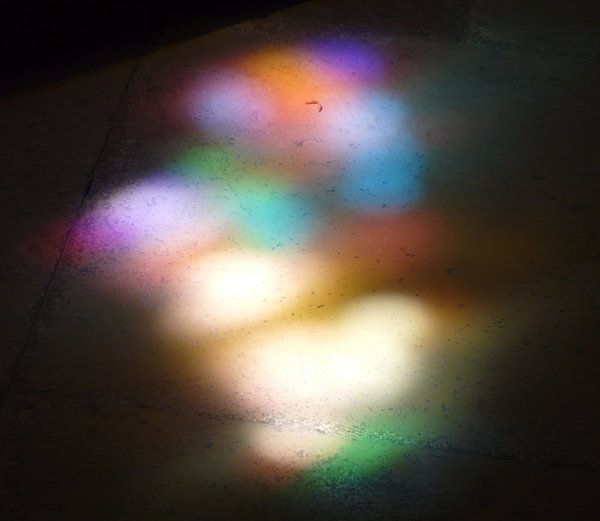
\includegraphics[height=6cm]{lichtspiel.jpg}}
\end{dispListing}
{\tcbset{reset}\tcbusetemp}

\end{docTcbKey}%【v5 20231101】v3 2023-1011 /v4 20231025
% Typically, but not necessarily, a |tcolorbox| is put inside a separate paragraph and has some vertical space before and after it.
This behavior is controlled by the keys \refKey{/tcb/before} and \refKey{/tcb/after}.

通常情况下,但不一定,|tcolorbox| 放置在单独的段落中,并且在它前后有一些垂直空间。这种行为由键 \refKey{/tcb/before} 和 \refKey{/tcb/after} 控制。

% 通常情况下,但不是必须地,一个|tcolorbox|盒子被放置在单独的段落中,在它%之前和之后
% 的前后有一些垂直空间。%
% 这种行为是由\refKey{/tcb/before}和\refKey{/tcb/after}控制。

\begin{marker}
Before version 4.40, the default setting for \refKey{/tcb/before}
and \refKey{/tcb/after} was given by \refKey{/tcb/autoparskip}.
Starting with version 4.40, the default setting is given by
\refKey{/tcb/before skip balanced} and \refKey{/tcb/after skip balanced}.\par
Note that old documents may need adaptions of page breaks.\par
Alternatively, the old default setting can be restored by using

% 版本4.40之前,\refKey{/tcb/before}和\refKey{/tcb/after}的默认设置由\refKey{/tcb/autoparskip}控制。%
% 从4.40开始, 默认设置由\refKey{/tcb/before skip balanced}和\refKey{/tcb/after skip balanced}控制。\par
% 请注意,旧文档可能需要调整分页。\par
% 或者,可以使用以下命令恢复旧的默认设置

在版本4.40之前,\refKey{/tcb/before}和\refKey{/tcb/after}的默认设置由\refKey{/tcb/autoparskip}给出。从版本4.40开始,默认设置由\refKey{/tcb/before skip balanced}和\refKey{/tcb/after skip balanced}给出。请注意,旧文档可能需要调整分页。或者,可以通过使用以下方式恢复旧的默认设置:
\begin{dispListing}
\tcbsetforeverylayer{autoparskip}
\end{dispListing}
inside the document preamble.

在文档导言区中。
\end{marker}

\begin{docTcbKey}{before}{=\meta{code}}{no default, initially see \refKey{/tcb/before skip balanced}}
Sets the \meta{code} which is executed before the colored box.
It is not used for floating boxes.
Also, it is not used, if the box follows a heading immediately
and \refKey{/tcb/ignore nobreak} is set to \docValue{false}.

设置在盒子绘制之前执行的 \meta{code}。它不用于浮动框。如果盒子紧接着标题而来并且 \refKey{/tcb/ignore nobreak} 被设置为 \docValue{false},也不会使用。

% \meta{code}将在盒子绘制前执行。此项不用于浮动盒子。另外一个不生效的情况:如果盒子之前紧跟着标题且\refKey{/tcb/ignore nobreak}设为\docValue{false}.
\end{docTcbKey}

\begin{docTcbKey}{after}{=\meta{code}}{no default, initially see \refKey{/tcb/after skip balanced}}
Sets the \meta{code} which is executed after the colored box.
It is not used for floating boxes.

\meta{code}将在盒子绘制后执行。此项不用于浮动盒子。
\end{docTcbKey}


\begin{docTcbKey}{nobeforeafter}{}{style, no value}
Abbreviation for clearing the keys |before| and |after|. The colored box
is not put into a paragraph and there is no space before or after the box.

% 清除“之前”和“之后”密钥的缩写。彩色框不放入段落中,并且框前后没有空格。

清除|before|和|after|的简写形式。盒子没有放入段落中,盒子之前或之后没有空间。\footnote{译注:用上后,多个盒子就不会分行了}
\begin{exdispExample}{nobeforeafter}
\tcbset{myone/.style={colback=LightGreen,colframe=DarkGreen,
equal height group=nobefaf,width=\linewidth/4,nobeforeafter}}
\begin{tcolorbox}[myone,title=Box 1]Box 1\end{tcolorbox}%
\begin{tcolorbox}[myone,title=Box 2]Box 2\end{tcolorbox}%
\begin{tcolorbox}[myone,title=Box 3]Box 3\end{tcolorbox}%
\begin{tcolorbox}[myone,title=Box 4]Box 4\end{tcolorbox}
\end{exdispExample}
\end{docTcbKey}



\begin{docTcbKey}{force nobeforeafter}{}{style, no value}
Forces the setting of \refKey{/tcb/nobeforeafter} even if
\refKey{/tcb/before} and \refKey{/tcb/after} are set to other values
later. Do not use this option globally unless you \emph{really} know what you do.
Note that embedded boxes do not inherit this forced clearance.

强制设置\refKey{/tcb/nobeforeafter},甚至\refKey{/tcb/before}和\refKey{/tcb/after}是在这个选项设置之后又设置的。不要全局使用此选项,除非您\emph{真}的知道在做什么。注意,嵌套的盒子不会继承此项设置。
\end{docTcbKey}


%%\clearpage

\begin{docTcbKey}[][doc new={2020-09-25}]{before skip balanced}{=\meta{glue}}{no default, initially |0.5\textbackslash baselineskip plus 2pt|}
Inserts some vertical space before the colored box. This style sets \refKey{/tcb/before}.\par
在盒子之前插入一些垂直空间。该样式设置 \refKey{/tcb/before}。\par
% 在 tcolorbox 盒子之前,插入一些竖直的空白。此项也会设置 \refKey{/tcb/before}。\par
If the depth of the
preceeding \TeX\ box is between |0pt| and |0.3\baselineskip|,
the distance between the \emph{baseline} of the preceeding \TeX\ box and the tcolorbox
ist set to \meta{glue}$+$|0.3\baselineskip|.\par
如果前面的 \TeX\ 盒子的深度在 |0pt| 和 |0.3\baselineskip| 之间,前面的 \TeX\ 盒子的 \emph{基线} 与 tcolorbox 之间的距离设置为 \meta{glue}$+$|0.3\baselineskip|。\par
% 如果要处理的 \TeX\ 盒子的深度介于 |0pt| 到 |0.3\baselineskip|,
% \TeX\ 盒子的 \emph{基线} 到 tcolorbox 盒子间的空白高为 \meta{glue}$+$|0.3\baselineskip|.\par
If the depth is larger, the distance of the preceeding \TeX\ box and the tcolorbox
ist set to \meta{glue}.\par
如果深度更大,则前面的 \TeX\ 盒子与 tcolorbox 之间的距离设置为 \meta{glue}。\par
Alternatively, see \refKey{/tcb/before skip} which ignores the \emph{baseline}.

 或者,查看 \refKey{/tcb/before skip},该选项忽略了 \emph{基线}。
% 如果深度更大些, 则 \TeX\ 盒子和 tcolorbox 盒子间的空白设为 \meta{glue}.\par
% 也可以参阅 \refKey{/tcb/before skip},它忽略 \emph{baseline}.

\begin{exdispExample*}{before_skip_balanced}{sbs,lefthand ratio=0.6}
Some text.
\begin{tcolorbox}[before skip balanced=1cm,
colframe=red!50!white]
This is a \textbf{tcolorbox}.
\end{tcolorbox}
\end{exdispExample*}
\end{docTcbKey}


\begin{docTcbKey}[][doc new={2020-09-25}]{after skip balanced}{=\meta{glue}}{no default, initially |0.5\textbackslash baselineskip plus 2pt|}
Inserts some vertical space of the given \meta{glue} after the colored box.
This style sets \refKey{/tcb/after}.
Additionally, |\prevdepth| is set to |0.3\baselineskip|. The following
\TeX\ box may enlarge the space by further glue to adjust its \emph{baseline}.
Alternatively, see \refKey{/tcb/after skip} which ignores the \emph{baseline}.

插入指定的竖直空白到盒子后,高度为 \meta{glue}。%
此项会设置 \refKey{/tcb/after}。%
此外, |\prevdepth| 设为 |0.3\baselineskip|。下面的 \TeX\ 盒子可以通过弹性%进一步弹性来
扩大空间以调整其\emph{基线}。%
另见 \refKey{/tcb/after skip},它忽略 \emph{baseline}。

\begin{exdispExample*}{after_skip_balanced}{sbs,lefthand ratio=0.6}
\begin{tcolorbox}[after skip balanced=1cm,
colframe=red!50!white]
This is a \textbf{tcolorbox}.
\end{tcolorbox}
Some text.
\end{exdispExample*}
\end{docTcbKey}



\begin{docTcbKey}[][doc new={2020-09-25}]{beforeafter skip balanced}{=\meta{glue}}{no default, initially |0.5\textbackslash baselineskip plus 2pt|}
插入一些指定高度为 \meta{glue} 的垂直空间到盒子的前面和后面。
此项会同时设置 \refKey{/tcb/before skip balanced} 和 \refKey{/tcb/after skip balanced}。
todo tikzpicture
\begin{exdispExample*}{beforeafter_skip_balanced}{sbs,lefthand ratio=0.6}
\newtcolorbox{doubleline}[1][]{
beforeafter skip balanced=0pt,
height=1.8\baselineskip,
enlarge top by=.1\baselineskip,
enlarge bottom by=.1\baselineskip,
colframe=blue!20,colback=blue!5,
size=small,valign upper=center,#1 }

\noindent\begin{tikzpicture}
\path[use as bounding box] (0,0)
rectangle (0.1,0.1);
\foreach \y in {0,1,...,9}  {
\draw[very thin,red]
(-0.2,-\y*\baselineskip) --
(\linewidth+0.2cm,-\y*\baselineskip); }
\end{tikzpicture}
line 1\par
\begin{doubleline}  Abc  \end{doubleline}
\begin{doubleline}  Def  \end{doubleline}
line 2g\par
\begin{doubleline}  Ghi  \end{doubleline}
line 3\par
line 4 g
\end{exdispExample*}
\end{docTcbKey}



%%\clearpage

\begin{docTcbKey}[][doc new and updated={2020-09-25}{2015-03-16}]{before skip}{=\meta{glue}}{style, no default}
在盒子之前插入指定高度\meta{glue}的垂直空间。%
此项会设置 \refKey{/tcb/before}。%
同 \refKey{/tcb/before skip balanced} 相比, 这个 \meta{glue} upper 部分的边缘,并不是到基线位置。
\begin{exdispExample*}{before_skip}{sbs,lefthand ratio=0.6}
Some text.
\begin{tcolorbox}[before skip=1cm,
colframe=red!50!white]
This is a \textbf{tcolorbox}.
\end{tcolorbox}

Some text.
\begin{tcolorbox}[before skip=0cm,
colframe=red!50!white]
This is a \textbf{tcolorbox}.
\end{tcolorbox}
\end{exdispExample*}
\end{docTcbKey}

\begin{docTcbKey}[][doc new and updated={2020-09-25}{2017-02-01}]{after skip}{=\meta{glue}}{style, no default}
在盒子之后插入指定高度\meta{glue}的垂直空间。%
此项会设置 \refKey{/tcb/after}.
同 \refKey{/tcb/after skip balanced} 相比, %
这个 \meta{glue} 是相对于 lower 部分的边缘,并不是到基线位置。%\footnote{译注:后面有空想下英文原文是否有误?}
\begin{exdispExample*}{after_skip}{sbs,lefthand ratio=0.6}
\begin{tcolorbox}[after skip=1cm,
colframe=red!50!white]
This is a \textbf{tcolorbox}.
\end{tcolorbox}
Some text.
\end{exdispExample*}
\end{docTcbKey}

\begin{docTcbKey}[][doc new=2014-10-10]{beforeafter skip}{=\meta{glue}}{style, no default}
Inserts some vertical space of the given \meta{glue} before \emph{and} after the colored box.
This style sets \refKey{/tcb/before skip} and \refKey{/tcb/after skip}.

在盒子的前后插入指定高度\meta{glue}的垂直空间。%
此项会设置 \refKey{/tcb/before skip} 和 \refKey{/tcb/after skip}。


\begin{exdispExample*}{beforeafter_skip}{sbs,lefthand ratio=0.6}
\tcbset{beforeafter skip=0pt,
colframe=red!50!white}

text before
\begin{tcolorbox}
This is a \textbf{tcolorbox}.
\end{tcolorbox}
\begin{tcolorbox}
Second box.
\end{tcolorbox}
text after
\end{exdispExample*}
\end{docTcbKey}



%%\clearpage

\begin{docTcbKey}[][doc new=2014-11-07]{left skip}{=\meta{length}}{style, no default, initially |0mm|}
Inserts some horizontal space of the given \meta{length} before the colored box.
This style sets \refKey{/tcb/grow to left by} with the negated \meta{length},
i.e. the bounding box and box width are changed.

在盒子前插入给定 \meta{length} 的水平空间。
此项会设定 \refKey{/tcb/grow to left by} 为 \meta{length} 的相反数,
i.e. 边界框和盒子宽度已更改。
\begin{exdispExample*}{left_skip}{sbs,lefthand ratio=0.6}
\noindent\rule{\linewidth}{2pt}

\begin{tcolorbox}[left skip=1cm,
colframe=red!50!white]
This is a \textbf{tcolorbox}.
\end{tcolorbox}
\end{exdispExample*}
\end{docTcbKey}

\begin{docTcbKey}[][doc new=2014-11-07]{right skip}{=\meta{length}}{style, no default, initially |0mm|}
Inserts some horizontal space of the given \meta{length} after the colored box.
This style sets \refKey{/tcb/grow to right by} with the negated \meta{length},
i.e. the bounding box and box width are changed.

在盒子{\bf 后}插入给定 \meta{length} 的水平空间。%
此项会设定  \refKey{/tcb/grow to right by} 为 \meta{length} 的相反数,
i.e. 边界框和盒子宽度已更改。
\begin{exdispExample*}{right_skip}{sbs,lefthand ratio=0.6}
\noindent\rule{\linewidth}{2pt}

\begin{tcolorbox}[right skip=1cm,
colframe=red!50!white]
This is a \textbf{tcolorbox}.
\end{tcolorbox}
\end{exdispExample*}
\end{docTcbKey}



\begin{docTcbKey}[][doc new=2014-10-10]{leftright skip}{=\meta{length}}{style, no default}
Inserts some horizontal space of the given \meta{length} before \emph{and} after the colored box.
This style changes the bounding box and the box width.

在盒子前后插入给定长度为 \meta{length} 的水平空间。
此样式更改边界盒子和盒子宽度。

\begin{exdispExample*}{leftright_skip}{sbs,lefthand ratio=0.6}
\noindent\rule{\linewidth}{2pt}

\begin{tcolorbox}[leftright skip=1cm,
colframe=red!50!white]
This is a \textbf{tcolorbox}.
\end{tcolorbox}
\end{exdispExample*}
\end{docTcbKey}


%%\clearpage

\begin{docTcbKey}[][doc updated=2017-02-01]{parskip}{}{style, no value}
This options is considered to be superseded by
\refKey{/tcb/before skip balanced} and \refKey{/tcb/after skip balanced}
(see note on page~\pageref{subsec:surroundings}).\par
Sets the keys |before| and |after| to values which are
recommended, if the package |parskip| \emph{is} used and there is no better
idea for |before| and |after|. This is similar to:

此项有考虑使用 \refKey{/tcb/before skip balanced} 和 \refKey{/tcb/after skip balanced} 取代。
(见~\pageref{subsec:surroundings}页).\par
将 |before| 和 |after| 的值设置为推荐的值,如果{使用}了 |parskip| 包且 |before| 和 |after| 的值没有更好的主意。效果类似于:
\begin{dispListing}
\tcbset{parskip/.style={before={\par\pagebreak[0]\parindent=0pt},
                after={\par}}}
\end{dispListing}
\end{docTcbKey}

\begin{docTcbKey}[][doc updated=2017-02-01]{noparskip}{}{style, no value}
This options is considered to be superseded by
\refKey{/tcb/before skip balanced} and \refKey{/tcb/after skip balanced}
(see note on page~\pageref{subsec:surroundings}).\par
Sets the keys |before| and |after| to values which are
recommended, if the package |parskip| is \emph{not} used and there is no better
idea for |before| and |after|. This is similar to:

此项有考虑使用 \refKey{/tcb/before skip balanced} 和 \refKey{/tcb/after skip balanced} 取代。
(见~\pageref{subsec:surroundings}页).\par
将 |before| 和 |after| 的值设置为推荐的值,如果{使用}了 |parskip| 包且 |before| 和 |after| 的值没有更好的主意。效果类似于:
\begin{dispListing}
\tcbset{noparskip/.style={before={\par\pagebreak[0]\smallskip\parindent=0pt},
                    after={\par\smallskip}}}
\end{dispListing}
\end{docTcbKey}



\begin{docTcbKey}{autoparskip}{}{style, no value}
This options is considered to be superseded by
\refKey{/tcb/before skip balanced} and \refKey{/tcb/after skip balanced}
(see note on page~\pageref{subsec:surroundings}).\par
Tries to detect the usage of the package |parskip| and sets
the keys |before| and |after| accordingly. Actually, the following is done:

这项可以考虑改用 \refKey{/tcb/before skip balanced} 和 \refKey{/tcb/after skip balanced} 替换(另见~\pageref{subsec:surroundings}~页)。\par
尝试检测 |parskip| 的使用情况, 并相应的设置 |before| 和 |after|。 实际上,完成了以下操作:

\begin{itemize}
\item 
If the length of |\parskip| is greater than |0pt| at the beginning of the document,
\refKey{/tcb/parskip} is executed. Here, the usage of package |parskip| is \emph{assumed}.

todo
如果在文档的开头 |\parskip| 的值大于|0pt|,%
\refKey{/tcb/parskip} 将会执行。 这里, 假定 |parskip| 引入\footnote{Here, the usage of package |parskip| is \emph{assumed}}。

\item 
Otherwise, if the length of |\parskip| is not greater than |0pt| at the beginning of the document,
\refKey{/tcb/noparskip} is executed. Here, the absence of package |parskip| is \emph{assumed}.
另外,如果在文档的开头 |\parskip| 的值不大于|0pt|,%
\refKey{/tcb/noparskip} 将会执行。 这里, 假定 |parskip| 没有使用\footnote{Here, the absence of package |parskip| is \emph{assumed}}。
\end{itemize}
\end{docTcbKey}




%%\clearpage

\begin{docTcbKey}{baseline}{=\meta{length}}{no default, initially |0pt|}
Used to set the |\pgfsetbaseline| value of the resulting |tcolorbox|.
设置结果盒子的%,同其他 \TeX\ 对象对齐用的
基线的值(|\pgfsetbaseline|)。

\begin{exdispExample}{baseline}
\tcbset{colframe=red!50!white,width=4cm,nobeforeafter}
Some text\dotfill
\begin{tcolorbox}[baseline=3mm]
第一行
\end{tcolorbox}
\begin{tcolorbox}[baseline=3mm]
第一行\\第二行
\end{tcolorbox}
\begin{tcolorbox}[baseline=4mm]
第一行\\第二行\\第三行
\end{tcolorbox}
\end{exdispExample}
\end{docTcbKey}




\begin{docTcbKey}[][doc new=2014-10-10]{box align}{=\meta{alignment}}{style, no default, initially |bottom|}
Used to set the \refKey{/tcb/baseline} value of the resulting |tcolorbox|.
Feasible values for \meta{alignment} are:

Used to set the \refKey{/tcb/baseline} value of the resulting |tcolorbox|.
Feasible values for \meta{alignment} are:  
\begin{itemize}
\item\docValue{bottom}: %alignment with the box bottom,
与盒子底部对齐,
\item\docValue{top}: %alignment with the box top,
与盒子顶部对齐,
\item\docValue{center}: %alignment with the box center,
与盒子中心对齐,
\item\docValue{base}: 
alignment with the box content base. This option
is not applicable for a \refEnv{tcolorbox} but for a \refCom{tcbox} only.
It is an alias for \refKey{/tcb/tcbox raise base}.
与盒子内容的基线对齐。此项不在 \refEnv{tcolorbox} 使用,仅在 \refCom{tcbox} 生效。
这是 \refKey{/tcb/tcbox raise base} 的别名。
\end{itemize}

\begin{exdispExample}{box_align_1}
\tcbset{colframe=red!50!white,width=4cm,nobeforeafter}
Some text\dotfill
\begin{tcolorbox}[box align=bottom]
bottom
\end{tcolorbox}
\begin{tcolorbox}[box align=bottom]
bottom\\bottom
\end{tcolorbox}
\begin{tcolorbox}
第一行\\第二行\\第三行
\end{tcolorbox}
\end{exdispExample}

\begin{exdispExample}{box_align_2}
\tcbset{colframe=red!50!white,width=4cm,nobeforeafter}
Some text\dotfill
\begin{tcolorbox}[box align=top]
top
\end{tcolorbox}
\begin{tcolorbox}[box align=top]
top\\top
\end{tcolorbox}
\begin{tcolorbox}
第一行\\第二行\\第三行
\end{tcolorbox}
\end{exdispExample}

\begin{exdispExample}{box_align_3}
\tcbset{colframe=red!50!white,width=4cm,nobeforeafter}
Some text\dotfill
\begin{tcolorbox}[box align=center]
center
\end{tcolorbox}
\begin{tcolorbox}[box align=center]
center\\center
\end{tcolorbox}
\begin{tcolorbox}
第一行\\第二行\\第三行
\end{tcolorbox}
\end{exdispExample}

\begin{exdispExample}{box_align_4}
\tcbset{colframe=red!50!white,nobeforeafter}
Some text\dotfill
\tcbox[nobeforeafter,box align=base]{base}
\tcbox[nobeforeafter,box align=base,size=fbox]{base}
\tcbox[nobeforeafter]{未设置}
\end{exdispExample}
\end{docTcbKey}





\begin{docTcbKey}[][doc new=2014-12-11]{ignore nobreak}{\colOpt{=true\textbar false}}{default |true|, initially |false|}
After a heading, \LaTeX\ tries to avoid a break by setting a |nobreak| boolean value.
Starting from version |3.33|, the \refKey{/tcb/before} respectively \refKey{/tcb/before skip}
settings are not used after a heading if \refKey{/tcb/ignore nobreak} is
set to \docValue{false}. For an unbreakable box, \refKey{/tcb/before nobreak} is used instead.
Further, a \refKey{/tcb/breakable} box will also try to
avoid a break between a heading and a directly following first part of a
break sequence.

在标题之后, 通过设置 |nobreak| ,\LaTeX\ 会尝试避免分页。
从版本 |3.33| 开始, 如果 \refKey{/tcb/ignore nobreak} 设置为 \docValue{false}, 那么 \refKey{/tcb/before} 和 \refKey{/tcb/before skip}
的设置在标题之后将不生效。%
对于一个不可分的盒子, 将使用 \refKey{/tcb/before nobreak} 替代使用。
将来, 一个设置了 \refKey{/tcb/breakable} 的盒子,将会尝试避免在标题和紧随其后的中断序列的第一部分之间中断。

Set \refKey{/tcb/ignore nobreak} to \docValue{true}, if |nobreak| should be
ignored as prior to version |3.33|. Also, such a setting may be used locally to
enforce the \refKey{/tcb/before} setting.
在版本 |3.33|,如果需要保留这个忽略 |nobreak| 的效果,将 \refKey{/tcb/ignore nobreak} 设置为 \docValue{true}。 此外,这样的设置可以在 locally 使用以强制设置 \refKey{/tcb/before} 。
\end{docTcbKey}

\begin{docTcbKey}[][doc new=2014-12-16]{before nobreak}{=\meta{code}}{no default, initially \cs{noindent}}
Sets the \meta{code} which is executed before the colored box if it
is unbreakable, if \refKey{/tcb/ignore nobreak} is not set, and if
the box follows a heading.

如果是不可以分的,设置 \meta{code} 在盒子之前执行, 如果没有设置 \refKey{/tcb/ignore nobreak} , 或如果盒子是跟随在标题之后。
\end{docTcbKey}



\begin{docTcbKey}[][doc new=2017-02-23]{parfillskip restore}{\colOpt{=true\textbar false}}{default |true|, initially |true|}
If this option is set to be |true|, the minimum value of |\parfillskip| is
tested at specific spots, if it is greater than |0pt|.
If so, |\parfillskip| is restored to |\@flushglue| which happens to be
the default value.

如果此项设置为 |true|, 则在特定点测试 |\parfillskip| 的最小值, 如果它大于 |0pt|.
如果是这样,|\parfillskip| 恢复到 |\@flushglue|, 这恰好是默认值。

These tests are executed for
这些判断将会在以下位置执行:
\refKey{/tcb/parskip},
\refKey{/tcb/noparskip},
\refKey{/tcb/after skip},
\refKey{/tcb/breakable}, and
\refEnv{tcbraster}.

This option was created to automatically
avoid overfull box warnings with |\parfillskip| changing packages.

创建此选项是为了自动避免 |\parfillskip| 改变包裹带来的 |overfull box| 警告 。
\end{docTcbKey}%【v5 20231101】 可以再看看,例子修改,分成几个文件  %v3 2023-1011 /v4 20231025
% 
Normally, every |tcolorbox| has a bounding box which fits exactly to the
dimensions of the outer frame. Therefore, \LaTeX\ reserves exactly the space
needed for the box.
This behavior can be changed by enlarging (or shrinking) the bounding box.
If the bounding box is enlarged, the |tcolorbox| will get some clearance
around it. If the bounding box is shrunk, i.\,e.\ enlarged with negative
values, the |tcolorbox| will overlap to other parts of the page.
For example, the |tcolorbox| could be stretched into the page margin.

通常,每个 |tcolorbox| 都有一个边界框,它恰好适合外部框架的尺寸。因此,\LaTeX\ 精确地保留了盒子所需的空间。 可以通过放大(或缩小)边界框来改变这种行为。 如果边界框被放大,|tcolorbox| 将在其周围获得一些间隙。 如果边界框被缩小,即用负值放大,|tcolorbox| 将与页面的其他部分重叠。 例如,|tcolorbox| 可以延伸到页面边缘。

% 通常,每个 |tcolorbox| 盒子有一个与其外框严丝合缝的边界盒子。%
% 因此,\LaTeX\ 保留了盒子所需的空间。%
% 可以通过扩大(或缩小)边界盒子来更改此空间。%
% 如果边界盒子被放大, 那么 |tcolorbox| 的周围将多出一些空间。 如果边界框缩小, i.\,e.\ 扩大一个负值, |tcolorbox| 将重叠到页面的其他部分。%
% 例如,|tcolorbox| 可能会突到页边距去。

\begin{marker}
The following examples use \refKey{/tcb/show bounding box} to display the actual bounding box. For this, the library \mylib{skins} has to be included and \refKey{/tcb/enhanced} has to be set.

以下示例使用\refKey{/tcb/show bounding box}来显示实际边界框。为此,必须包含库\mylib{skins}并设置\refKey{/tcb/enhanced}。
% 以下示例使用 \refKey{/tcb/show bounding box} 来显示实际的边界框。为此,必须包含库 \mylib{skins} 并且必须设置 \refKey{/tcb/enhanced}。
\end{marker}



\subsubsection{Shifting Bounding Box Borders\\移动边界盒子的边框}

\begin{docTcbKey}{enlarge top initially by}{=\meta{length}}{no default, initially |0mm|}
Enlarges the bounding box distance to the top of the box by \meta{length}.
If the box is \emph{breakable}, only the first box of the break sequence
gets enlarged. \refKey{/tcb/enlarge top by} overwrites this key.

将边框顶部的边界框距离增加\meta{length}。如果该盒子是\emph{可分页的},则仅对分页序列的第一个框进行扩展。 \refKey{/tcb/enlarge top by} 覆盖此键。 

% 扩大边界盒子同 |tcolorbox| 盒子的顶部的距离 \meta{length}。
% 如果 |tcolorbox| 盒子是\emph{可分的}, 只有中断序列的第一个盒子的扩大会生效。 
\refKey{/tcb/enlarge top by} 会覆盖这个设置。
\begin{exdispExample}{enlarge_top_initially_by}
\tcbset{colframe=blue!75!black,colback=white}

\begin{tcolorbox}[enlarge top initially by=-5mm]
This is a \textbf{tcolorbox}.
\end{tcolorbox}
\begin{tcolorbox}[enlarge top initially by=5mm,enhanced,show bounding box]
This is a \textbf{tcolorbox}.
\end{tcolorbox}
\end{exdispExample}
\end{docTcbKey}

\begin{tcolorbox}[nobeforeafter]
\textbf{tcolorbox} a.
\end{tcolorbox}
\begin{tcolorbox}[nobeforeafter]
\textbf{tcolorbox} b.
\end{tcolorbox}




\begin{docTcbKey}{enlarge bottom finally by}{=\meta{length}}{no default, initially |0mm|}
Enlarges the bounding box distance to the bottom of the box by \meta{length}.
If the box is \emph{breakable}, only the last box of the break sequence
gets enlarged. \refKey{/tcb/enlarge bottom by} overwrites this key.

通过\meta{length}来增加盒子底部的边界距离。如果该盒子是\emph{可分割}的,那么只有分割序列的最后一个盒子会被放大。 \refKey{/tcb/enlarge bottom by} 会覆盖此关键字。

% 扩大边界盒子同 |tcolorbox| 盒子的底部的距离 \meta{length}。%
% 如果盒子是 \emph{可中断的}, 只有中断序列的最后一部分得到扩大。
% \refKey{/tcb/enlarge bottom by} 会覆盖这个设置。
\begin{exdispExample}{enlarge_bottom_finally_by}
\tcbset{colframe=blue!75!black,colback=white}

\begin{tcolorbox}[enlarge bottom finally by=5mm]
This is a \textbf{tcolorbox}.
\end{tcolorbox}
\begin{tcolorbox}[enlarge bottom finally by=-5mm,enhanced,show bounding box]
This is a \textbf{tcolorbox}.
\end{tcolorbox}
\end{exdispExample}
\end{docTcbKey}

%%\clearpage




\begin{docTcbKey}{enlarge top at break by}{=\meta{length}}{no default, initially \texttt{0mm}}
Enlarges the bounding box distance to the top of the box by \meta{length},
\emph{if} the box is \refKey{/tcb/breakable}.
In this case, it is applied to \emph{middle} and \emph{last} parts in a
break sequence.
\refKey{/tcb/enlarge top by} overwrites this key.

\emph{如果}盒子是 \refKey{/tcb/breakable}的,扩大边界盒子同 |tcolorbox| 盒子的顶部的距离 \meta{length}。这种情况下, 它在 \emph{中间}和\emph{最后}的中断序列部分生效。 \refKey{/tcb/enlarge top by} 会覆盖此项设置。
\end{docTcbKey}


\begin{docTcbKey}{enlarge bottom at break by}{=\meta{length}}{no default, initially \texttt{0mm}}
Enlarges the bounding box distance to the bottom of the box by \meta{length},
\emph{if} the box is \refKey{/tcb/breakable}.
In this case, it is applied to \emph{first} and \emph{middle} parts in a
break sequence. \refKey{/tcb/enlarge bottom by} overwrites this key.

\emph{如果}盒子是 \refKey{/tcb/breakable}的,扩大边界盒子同 |tcolorbox| 盒子的底部的距离 \meta{length}。
这种情况下, 它在 \emph{首个}和\emph{中间}的中断序列部分生效。
\refKey{/tcb/enlarge bottom by} 会覆盖此项设置。
\end{docTcbKey}




\begin{docTcbKey}{enlarge top by}{=\meta{length}}{no default, initially |0mm|}

Enlarges the bounding box distance to the top of the box by \meta{length}.
\refKey{/tcb/enlarge top initially by} and
\refKey{/tcb/enlarge top at break by} are set to \meta{length}.

扩大边界盒子同 |tcolorbox| 盒子的{\bf 顶}部的距离 \meta{length}。
\refKey{/tcb/enlarge top initially by} 和
\refKey{/tcb/enlarge top at break by} 也会被设置为 \meta{length}。
\end{docTcbKey}


\begin{docTcbKey}{enlarge bottom by}{=\meta{length}}{no default, initially |0mm|}
Enlarges the bounding box distance to the bottom of the box by \meta{length}.
\refKey{/tcb/enlarge bottom finally by} and
\refKey{/tcb/enlarge bottom at break by} are set to \meta{length}.

扩大边界盒子同 |tcolorbox| 盒子的{\bf 底}部的距离 \meta{length}。
\refKey{/tcb/enlarge bottom finally by} 和
\refKey{/tcb/enlarge bottom at break by} 也会被设为 \meta{length}.
\end{docTcbKey}



\begin{docTcbKey}{enlarge left by}{=\meta{length}}{no default, initially |0mm|}
Enlarges the bounding box distance to the left side of the box by \meta{length}.

扩大边界盒子同 |tcolorbox| 盒子的{\bf 左侧}的距离 \meta{length}。
\begin{exdispExample}[safety=2cm]{enlarge_left_by}
\tcbset{colframe=blue!75!black,colback=white}

\begin{tcolorbox}[enlarge left by=2cm,width=5cm,enhanced,show bounding box]
This is a \textbf{tcolorbox}.
\end{tcolorbox}
\begin{tcolorbox}[enlarge left by=-2cm,width=\linewidth+2cm]
This is a \textbf{tcolorbox}.
\end{tcolorbox}
\end{exdispExample}
\end{docTcbKey}

\begin{docTcbKey}{enlarge right by}{=\meta{length}}{no default, initially |0mm|}
Enlarges the bounding box distance to the right side of the box by \meta{length}.

扩大边界盒子同 |tcolorbox| 盒子的{\bf 右侧}的距离 \meta{length}。
\begin{exdispExample}[safety=2cm]{enlarge_right_by}
\tcbset{colframe=blue!75!black,colback=white}

\begin{tcolorbox}[enlarge right by=-2cm,width=\linewidth+2cm,
enhanced,show bounding box]
\textbf{tcolorbox}缩小了同右侧的距离到负数,就突出到右边了.
\end{tcolorbox}
\begin{tcolorbox}[enlarge right by=2cm,width=\linewidth-2cm]
This is a \textbf{tcolorbox}.
\end{tcolorbox}
\end{exdispExample}
\end{docTcbKey}




%%\clearpage
\begin{docTcbKey}{enlarge by}{=\meta{length}}{no default, initially |0mm|}
Enlarges the bounding box distance to all sides of the box by \meta{length}.

扩大边界盒子同 |tcolorbox| 盒子的{\bf 四侧}的距离 \meta{length}。
\begin{exdispExample}{enlarge_by}
\tcbset{colframe=blue!75!black,colback=white,width=5cm,nobeforeafter}

\begin{tcolorbox}
This is a \textbf{tcolorbox}.
\end{tcolorbox}
\begin{tcolorbox}[enlarge by=5mm,enhanced,show bounding box]
This is a \textbf{tcolorbox}.
\end{tcolorbox}
\end{exdispExample}
\end{docTcbKey}





\begin{docTcbKey}{grow to left by}{=\meta{length}}{no default, initially |0mm|}
Enlarges the current box width by \meta{length} and
enlarges (shrinks) the bounding box distance to the left side of the box by
$-$\meta{length}. Also see \refKey{/tcb/left skip}.

扩大当前盒子的宽度\meta{length},并扩大边界盒子到左侧的距离为
$-$\meta{length}。\footnote{突出到左侧了} 另见 \refKey{/tcb/left skip}。
\begin{exdispExample}[safety=2cm]{grow_to_left_by}
\tcbset{colframe=blue!75!black,colback=white}

\begin{tcolorbox}[width=5cm,grow to left by=2cm,enhanced,show bounding box]
This is a \textbf{tcolorbox} with a width of 7cm.
\end{tcolorbox}
\end{exdispExample}
\end{docTcbKey}

\begin{docTcbKey}{grow to right by}{=\meta{length}}{no default, initially |0mm|}
Enlarges the current box width by \meta{length} and
enlarges (shrinks) the bounding box distance to the right side of the box by
$-$\meta{length}. Also see \refKey{/tcb/right skip}.

扩大当前盒子的宽度\meta{length},并扩大边界盒子到右侧的距离为
$-$\meta{length}。\footnote{突出到右侧了} 另见 \refKey{/tcb/right skip}。
\begin{exdispExample}[safety=2cm]{grow_to_right_by}
\tcbset{colframe=blue!75!black,colback=white}

\begin{tcolorbox}[grow to right by=2cm,enhanced,show bounding box]
This is a \textbf{tcolorbox}.
\end{tcolorbox}

\bigskip

\begin{tcolorbox}[grow to right by=2cm,grow to left by=1cm,
enhanced,show bounding box]
This is a \textbf{tcolorbox}.
\end{tcolorbox}
\end{exdispExample}
\end{docTcbKey}

%%\clearpage


\begin{docTcbKey}[][doc new=2018-03-22]{grow sidewards by}{=\meta{length}}{no default, initially |0mm|}
Shortcut for setting \refKey{/tcb/grow to left by} and \refKey{/tcb/grow to right by}
to \meta{length}. Also see \refKey{/tcb/oversize} and \refKey{/tcb/spread sidewards}.

同时设置 \refKey{/tcb/grow to left by} 和 \refKey{/tcb/grow to right by} 到\meta{length} 的简写形式。另见 \refKey{/tcb/oversize} 和 \refKey{/tcb/spread sidewards}.
\begin{exdispExample}[safety=2cm]{grow_sidewards_by}
\tcbset{colframe=blue!75!black,colback=white}

\begin{tcolorbox}[grow sidewards by=2cm,enhanced,show bounding box]
This is a \textbf{tcolorbox}.
\end{tcolorbox}
\end{exdispExample}
\end{docTcbKey}




\subsubsection{Box Alignment\\盒子的对齐}

\begin{docTcbKey}[][doc new=2015-11-20]{flush left}{}{style, no value}
Enlarges the bounding box to the right side to fill the line completely.

左对齐效果,扩大边界盒子完全填充到右侧。
\begin{exdispExample}{flush_left}
\tcbset{colframe=blue!75!black,colback=white}

\begin{tcolorbox}[flush left,width=5cm,enhanced,show bounding box]
This is a \textbf{tcolorbox}.
\end{tcolorbox}
\end{exdispExample}
\end{docTcbKey}


\begin{docTcbKey}[][doc new=2015-11-20]{flush right}{}{style, no value}
Enlarges the bounding box to the left side to fill the line completely.

右对齐效果,扩大边界盒子完全填充到左侧。
\begin{exdispExample}{flush_right}
\tcbset{colframe=blue!75!black,colback=white}

\begin{tcolorbox}[flush right,width=5cm,enhanced,show bounding box]
This is a \textbf{tcolorbox}.
\end{tcolorbox}
\end{exdispExample}
\end{docTcbKey}


\begin{docTcbKey}[][doc new=2015-11-20]{center}{}{style, no value}
Enlarges the bounding box equally to both sides to fill the line completely.

居中对齐效果,扩大边界盒子完全填充到两侧。
\begin{exdispExample}{center}
\tcbset{colframe=blue!75!black,colback=white}

\begin{tcolorbox}[center,width=5cm,enhanced,show bounding box]
This is a \textbf{tcolorbox}.
\end{tcolorbox}
\end{exdispExample}
\end{docTcbKey}




%%\clearpage

\subsubsection{Toggle Enlargements}

\begin{docTcbKey}[][doc updated=2015-11-13]{toggle enlargement}{=\meta{toggle preset}}{默认 |evenpage|(偶), initially |none|}
According to the \meta{toggle preset}, the left and the right enlargements of
the bounding box are switched or not. Feasible values are:

依据 \meta{toggle preset} 的值, 对边界盒子的左边和右边的增加空间的设置进行交换或不交换。可设的值有:
\begin{itemize}
\item\docValue{none}: %no switching.
不切换。
\item\docValue{forced}: %the values of the left and right enlargement are switched.
强制将边界盒子的左边和右边的增加空间的设置进行交换。
\item\docValue{evenpage}: 
if the page is an even page, the values of the left and    right enlargement are switched. This value also sets    \refKey{/tcb/check odd page} to |true|.

如果当前页是偶数页, 将边界盒子的左边和右边的增加空间的设置进行交换。这项值也会将  \refKey{/tcb/check odd page} 设置为 |true|.
\end{itemize}
\begin{marker}
See \refKey{/tcb/toggle left and right} to toggle geometry settings.
见 \refKey{/tcb/toggle left and right} 来切换几何设置。
\end{marker}

\begin{dispExample}
\tcbset{colframe=blue!75!black,colback=white,
grow to left by=20mm,%突出左侧
grow to right by=-5mm%右侧凹着
}

\begin{tcolorbox}[toggle enlargement=none
,enhanced,show bounding box]
设置为 |toggle enlargement=none|,不切换
\end{tcolorbox}
\begin{tcolorbox}[toggle enlargement=forced]
设置为 |toggle enlargement=forced|,强制切换
\end{tcolorbox}
\begin{tcolorbox}[toggle enlargement=evenpage]
设置为 |toggle enlargement=evenpage|,偶数页才切换。当前页是 \tcbifoddpage{奇}{偶} 数页。因此, 左边的增加空间的设置 \tcbifoddpage{不会}{会}切换。
\end{tcolorbox}
\end{dispExample}

\begin{dispListing}
\begin{tcolorbox}[colframe=red!60!black,colback=red!15!white,
fonttitle=\bfseries,title=Floating box from \texttt{toggle enlargement},
width=\textwidth
,grow to right by=2cm%突出到右边
,toggle enlargement%默认是偶数页
,float=t]
当前页是\tcbifoddpage{奇}{偶}数页。%
因此, 左边的增加空间的设置 \tcbifoddpage{不会}{会}切换。%
这个盒子,在奇数页是突出到右边,在偶数页是突出到左边。%
本文档是one-sided文档 -- 这项特性只在two-sided%
\footnote{译注:即双面打印,%
奇数和偶数页的文档内容的左右边距是不同的,以用于装订。}%
文档中生效。
\end{tcolorbox}
\end{dispListing}
\tcbusetemp
\end{docTcbKey}





%%\clearpage

\subsubsection{Spread Box to Page Borders\\盒子扩张到页面边缘}

\begin{marker} 
The following border options are \emph{not} applicable to nested boxes, boxes insides tables, etc.
For boxes inside lists, the options \emph{may} work, but not necessarily.
Also, boxes should be set with |\noindent| and full width.

以下的 border 选项对嵌套的盒子, 在表格中的盒子\emph{不}起作用, etc.
对于列表中的盒子,这些选项\emph{可以}工作, 但没必要。
另外,盒子需要设置 |\noindent| 来达到全宽。
\end{marker}

\begin{docTcbKey}[][doc new=2017-02-13]{spread inwards}{\colOpt{=\meta{length}}}{default |0pt|, initially unset}
Enlarges the current box width to match the inner page border (left-handed side for one-sided
documents). If the optional \meta{length} is greater than |0pt|, the box
grows over the border, if \meta{length} is lower than |0pt|, there is a
margin between box and page border.
\refKey{/tcb/toggle enlargement} is set automatically.

扩张当前盒子的宽度到书本的内页边缘(对单面文档是在左侧).如果选项的值\meta{length}是大于 |0pt|, 那么盒子将穿过页面的边缘, 如果\meta{length}是小于|0pt|,那么在盒子和页面边缘就有一段面边空白。会自动设置 \refKey{/tcb/toggle enlargement} 。
\begin{dispListing}
\begin{tcolorbox}[enhanced,spread inwards,
colframe=blue!75!black,colback=white,show bounding box]
扩张当前盒子的宽度到书本的内页边缘 (对单面文档是在左侧).(|spread inwards|)
\end{tcolorbox}

\begin{tcolorbox}[enhanced,spread inwards=2em,
colframe=blue!75!black,colback=white,show bounding box]
前面的内容穿过边缘了(|spread inwards=2em,|)。
\end{tcolorbox}

\begin{tcolorbox}[enhanced,spread inwards=-2em,
colframe=blue!75!black,colback=white,show bounding box]
在盒子和页面边缘就有一段面边空白。(|spread inwards=-2em,|)。
\end{tcolorbox}
\end{dispListing}
{\tcbusetemp}
\end{docTcbKey}



\begin{docTcbKey}[][doc new=2017-02-13]{spread outwards}{\colOpt{=\meta{length}}}{default |0pt|, initially unset}
Enlarges the current box width to match the outer page border (right-handed side for one-sided
documents). If the optional \meta{length} is greater than |0pt|, the box
grows over the border, if \meta{length} is lower than |0pt|, there is a
margin between box and page border.
\refKey{/tcb/toggle enlargement} is set automatically.

扩张当前盒子的宽度到书本的内页边缘(对单面文档是在右侧)。如果选项的值\meta{length}是大于 |0pt|, 那么盒子将穿过页面的边缘, 如果\meta{length}是小于|0pt|,那么在盒子和页面边缘就有一段空白。会自动设置 \refKey{/tcb/toggle enlargement} 。

\begin{dispListing}
\begin{tcolorbox}[enhanced,spread outwards,
colframe=blue!75!black,colback=white,show bounding box]
This is a \textbf{tcolorbox}.
\end{tcolorbox}
\end{dispListing}
{\tcbusetemp}
\end{docTcbKey}


\begin{docTcbKey}[][doc new=2017-02-13]{move upwards}{\colOpt{=\meta{length}}}{default |0pt|, initially unset}
Starts a new page with the box at the very top page border.
If the optional \meta{length} is greater than |0pt|, the box
moves over the border, if \meta{length} is lower than |0pt|, there is a
margin between box and page border.

新起一页,将盒子放在新页面的最顶部。%
如果选项的值\meta{length}是大于 |0pt|, 那么盒子将穿过页面的边缘, 如果\meta{length}是小于|0pt|,那么在盒子和页面边缘就有一段空白。
\end{docTcbKey}


\begin{docTcbKey}[][doc new=2017-02-13]{move upwards*}{\colOpt{=\meta{length}}}{default |0pt|, initially unset}
同\refKey{/tcb/move upwards}一样,但少了新起一页的操作。
\end{docTcbKey}




\begin{docTcbKey}[][doc new=2017-02-13]{fill downwards}{\colOpt{=\meta{length}}}{default |0pt|, initially unset}
Enlarges the height of the box until the very bottom page border.
The library \mylib{breakable} has to be loaded, and
\refKey{/tcb/height fill} is set automatically.
If the optional \meta{length} is greater than |0pt|, the box
moves over the border, if \meta{length} is lower than |0pt|, there is a
margin between box and page border.

扩张当前盒子的宽度到书本的底部边缘。%
需要加载 \mylib{breakable} 库, 且会自动设置\refKey{/tcb/height fill} 。%
如果选项的值\meta{length}是大于 |0pt|, 那么盒子将穿过页面的边缘, 如果\meta{length}是小于|0pt|,那么在盒子和页面边缘就有一段空白。
\begin{dispListing}
\begin{tcolorbox}[enhanced,fill downwards,
colframe=blue!75!black,colback=white,show bounding box]
扩张当前盒子的宽度到书本的底部边缘。
\end{tcolorbox}
\end{dispListing}
{\tcbusetemp}
\end{docTcbKey}


\begin{tcolorbox}[enhanced,spread upwards,sharp corners=north,height=3cm,
colframe=blue!75!black,interior style={top color=blue!50,bottom color=white}]
这是\enquote{spread upwards}的例子。 
\end{tcolorbox}
\begin{docTcbKey}[][doc new=2017-02-13]{spread upwards}{\colOpt{=\meta{length}}}{default |0pt|, initially unset}
组合,同时将\meta{length}设到
\refKey{/tcb/move upwards}, \refKey{/tcb/spread inwards}, 和 \refKey{/tcb/spread outwards}.
\begin{dispListing}
\begin{tcolorbox}[enhanced,spread upwards,sharp corners=north,height=3cm,
colframe=blue!75!black,interior style={top color=blue!50,bottom color=white}]
这是 \enquote{spread upwards} 的例子。
\end{tcolorbox}
\end{dispListing}
\end{docTcbKey}


\begin{docTcbKey}[][doc new=2017-02-13]{spread upwards*}{\colOpt{=\meta{length}}}{default |0pt|, initially unset}
同\refKey{/tcb/move upwards}一样,但不会新起一页。
\end{docTcbKey}




\begin{docTcbKey}[][doc new=2017-02-13]{spread sidewards}{\colOpt{=\meta{length}}}{default |0pt|, initially unset}
Combination of \refKey{/tcb/spread inwards} and \refKey{/tcb/spread outwards}.
The optional \meta{length} is used for all these keys.
Also see \refKey{/tcb/oversize} and \refKey{/tcb/grow sidewards by}.

\meta{length}被同时设置到 \refKey{/tcb/spread inwards} 和 \refKey{/tcb/spread outwards}。另见 \refKey{/tcb/oversize} 和 \refKey{/tcb/grow sidewards by}.
\begin{dispListing}
\begin{tcolorbox}[enhanced,spread sidewards,
colframe=blue!75!black,colback=white,show bounding box]
向左右两侧突出了。
\end{tcolorbox}
\end{dispListing}
{\tcbusetemp}
\end{docTcbKey}


\begin{docTcbKey}[][doc new=2017-02-13]{spread}{\colOpt{=\meta{length}}}{default |0pt|, initially unset}
Combination of
\refKey{/tcb/move upwards}, \refKey{/tcb/fill downwards}, \refKey{/tcb/spread inwards},
and \refKey{/tcb/spread outwards}.
Such, the box fills the whole page.
The optional \meta{length} is used for all these keys.

组合了 \refKey{/tcb/move upwards}, \refKey{/tcb/fill downwards}, \refKey{/tcb/spread inwards},和 \refKey{/tcb/spread outwards}。
这样,盒子就填满了整个页面。
\meta{length} 被同时设置到这些选项。
\end{docTcbKey}




\begin{docTcbKey}[][doc new=2017-02-13]{spread downwards}{\colOpt{=\meta{length}}}{default |0pt|, initially unset}
Combination of
\refKey{/tcb/fill downwards}, \refKey{/tcb/spread inwards}, and \refKey{/tcb/spread outwards}.
The optional \meta{length} is used for all these keys.

组合使用 \refKey{/tcb/fill downwards}, \refKey{/tcb/spread inwards}, 和 \refKey{/tcb/spread outwards}.
\meta{length} 被同时设置到这些选项。
\begin{dispListing}
\begin{tcolorbox}[enhanced,spread downwards,sharp corners=south,
colframe=red!75!black,interior style={top color=white,bottom color=red!50}]
This is an example for \enquote{spread downwards}.
\end{tcolorbox}
\end{dispListing}
\end{docTcbKey}
\begin{tcolorbox}[enhanced,spread downwards,sharp corners=south,
colframe=red!75!black,interior style={top color=white,bottom color=red!50}]
This is an example for \enquote{spread downwards}.
\end{tcolorbox}






%%\clearpage

\subsubsection{Box Extrusion\\挤压盒子}

\begin{marker}
The following keys should not be used with breakable boxes or boxes with a
lower part.

以下选项不应在可分盒子或带有lower部分的盒子内使用。
\end{marker}

\begin{docTcbKey}{shrink tight}{}{style, no value, initially unset}
The total colored box is shrunk to the dimensions of the upper
part. There should be no lower part and no title.
This style sets the \refKey{/tcb/boxsep} to |0pt| and other geometry keys
to fitting values. This option is likely to be used with the following
extrusion keys.

整个盒子缩小到upper部分的尺寸。不应有lower部分和标题。
此样式会将 \refKey{/tcb/boxsep} 设置为 |0pt|,以及一些其他几何设置。此选项可能与以下挤压键一起使用。
\begin{exdispExample}{shrink_tight}
\tcbset{colframe=blue!75!black,colback=white,arc=0mm,boxrule=0.4pt,
    nobeforeafter,tcbox raise base,shrink tight}

\begin{tcolorbox}
This is a \textbf{tcolorbox}.
\end{tcolorbox}

Lorem \tcbox{ipsum} dolor sit amet, consectetuer adipiscing elit.
\end{exdispExample}

\begin{exdispExample}{shrink_tight2}
\tcbset{colframe=blue!75!black,colback=white,arc=0mm,boxrule=0.4pt,
        shrink tight}

\begin{tcolorbox}
This is a \textbf{tcolorbox}.
\end{tcolorbox}

Lorem \tcbox{ipsum} dolor sit amet, consectetuer adipiscing elit.
\end{exdispExample}
\end{docTcbKey}  

% extrude
% ① (force out) 挤出 jǐchū ‹toothpaste, glue, icing›; 压出 yāchū ‹pasta›
% ② (shape) 压制 yāzhì ‹plastic, metal›
\begin{docTcbKey}[][doc updated=2014-09-19]{extrude left by}{=\meta{length}}{style, no default, initially unset}
The (upper part of the) colored box is extruded by the given \meta{length} to the left side.
The inner width and the bounding box is kept unchanged and the operation
is additive!

(upper部分)盒子向左挤出 \meta{length} 空间\footnote{译注:这部分有点像零宽的盒子效果。}。内部宽度和边界盒子保持不变,挤出是额外的!
\begin{exdispExample}{extrude_left_by}
\tcbset{enhanced,colframe=red,colback=yellow!25!white,
frame style={opacity=0.25},interior style={opacity=0.5},
nobeforeafter,tcbox raise base,shrink tight,extrude by=2mm}

Lorem ipsum dolor sit amet, consectetuer adipiscing elit. Ut purus elit,
vestibulum ut, placerat ac, adipiscing vitae, felis.
\tcbox[extrude left by=1cm]{Curabitur} dictum gravida mauris.
Nam arcu libero, nonummy eget, consectetuer id, vulputate a, magna.
\end{exdispExample}

\begin{exdispExample}{extrude_left_by2}
\tcbset{enhanced,colframe=red,colback=yellow!25!white,
frame style={opacity=0.25},interior style={opacity=0.5},
nobeforeafter,tcbox raise base,shrink tight,extrude by=2mm}

Lorem ipsum dolor sit amet, consectetuer adipiscing elit. Ut purus elit,
vestibulum ut, placerat ac, adipiscing vitae, felis.
\tcbox[extrude left by=1cm,,show bounding box]{Curabitur} dictum gravida mauris.
Nam arcu libero, nonummy eget, consectetuer id, vulputate a, magna.
\end{exdispExample}

\end{docTcbKey}

\begin{docTcbKey}[][doc updated=2014-09-19]{extrude right by}{=\meta{length}}{style, no default, initially unset}
The (upper part of the) colored box is extruded by the given \meta{length} to the right side.
The inner width and the bounding box is kept unchanged and the operation
is additive!

(upper部分)盒子向{\bf 右}挤出 \meta{length} 空间%\footnote{译注:这部分有点像零宽的盒子效果。}
。内部宽度和边界盒子保持不变,挤出是额外的!
\begin{exdispExample}{extrude_right_by}
\tcbset{enhanced,colframe=red,colback=yellow!25!white,
frame style={opacity=0.25},interior style={opacity=0.5},
nobeforeafter,tcbox raise base,shrink tight,extrude by=2mm}

Lorem ipsum dolor sit amet, consectetuer adipiscing elit. Ut purus elit,
vestibulum ut, placerat ac, adipiscing vitae, felis.
\tcbox[extrude right by=1cm]{Curabitur} dictum gravida mauris.
Nam arcu libero, nonummy eget, consectetuer id, vulputate a, magna.
\end{exdispExample}
\end{docTcbKey}

%%\clearpage
\begin{docTcbKey}{extrude top by}{=\meta{length}}{style, no default, initially unset}
The (upper part of the) colored box is extruded by the given \meta{length} to the top side.
The inner width and the bounding box is kept unchanged and the operation
is additive!

(upper部分)盒子向{\bf 上}挤出 \meta{length} 空间%\footnote{译注:这部分有点像零宽的盒子效果。}
。内部宽度和边界盒子保持不变,挤出是额外的!
\begin{exdispExample}{extrude_top_by}
\tcbset{enhanced,colframe=red,colback=yellow!25!white,
frame style={opacity=0.25},interior style={opacity=0.5},
nobeforeafter,tcbox raise base,shrink tight,extrude by=2mm}

Lorem ipsum dolor sit amet, consectetuer adipiscing elit. Ut purus elit,
vestibulum ut, placerat ac, adipiscing vitae, felis.
\tcbox[extrude top by=1cm]{Curabitur} dictum gravida mauris.
Nam arcu libero, nonummy eget, consectetuer id, vulputate a, magna.
\end{exdispExample}
\end{docTcbKey}

\begin{docTcbKey}{extrude bottom by}{=\meta{length}}{style, no default, initially unset}
The (upper part of the) colored box is extruded by the given \meta{length} to the bottom side.
The inner width and the bounding box is kept unchanged and the operation
is additive!

(upper部分)盒子向{\bf 下}挤出 \meta{length} 空间%\footnote{译注:这部分有点像零宽的盒子效果。}
。内部宽度和边界盒子保持不变,挤出是额外的!
\begin{exdispExample}[safety=1cm]{extrude_bottom_by}
\tcbset{enhanced,colframe=red,colback=yellow!25!white,
frame style={opacity=0.25},interior style={opacity=0.5},
nobeforeafter,tcbox raise base,shrink tight,extrude by=2mm}

Lorem ipsum dolor sit amet, consectetuer adipiscing elit. Ut purus elit,
vestibulum ut, placerat ac, adipiscing vitae, felis.
\tcbox[extrude bottom by=1cm]{Curabitur} dictum gravida mauris.
Nam arcu libero, nonummy eget, consectetuer id, vulputate a, magna.
\end{exdispExample}
\end{docTcbKey}



\begin{docTcbKey}{extrude by}{=\meta{length}}{style, no default, initially unset}
The (upper part of the) colored box is extruded by the given \meta{length} to all sides.
The inner width and the bounding box is kept unchanged and the operation
is additive!

(upper部分)盒子向{\bf 四周}都挤出 \meta{length} 空间%\footnote{译注:这部分有点像零宽的盒子效果。}
。内部宽度和边界盒子保持不变,挤出是额外的!
\begin{exdispExample}{extrude_by}
\tcbset{enhanced,colframe=red,colback=yellow!25!white,
frame style={opacity=0.25},interior style={opacity=0.5},
nobeforeafter,tcbox raise base,shrink tight,extrude by=2mm}

Lorem ipsum dolor sit amet, consectetuer adipiscing elit. Ut purus elit,
vestibulum ut, placerat ac, adipiscing vitae, felis. \tcbox{Curabitur} dictum
gravida mauris. \tcbox[colframe=Green,interior style={opacity=0.0}]{Nam}
arcu libero, nonummy eget, consectetuer id, \tcbox{vulputate} a, magna. Donec
vehicula augue eu neque. Pellentesque habitant morbi tristique senectus et netus
et malesuada fames ac turpis egestas. \tcbox{Mauris ut leo.}
\end{exdispExample}
\end{docTcbKey}%【v5 20231102】%v3 2023-1011 不错的效果 /v4 20231025 todo 将例子修改下更好看
% A |tcolorbox| may contain another |tcolorbox| and so on. The package
takes track of the nesting level using a counter |tcblayer|. Counter values
may be used for doing some fancy things, but you should never change
the counter value yourself.

一个|tcolorbox| 可以包含另一个 |tcolorbox|,以此类推。该包会使用计数器 |tcblayer| 来跟踪嵌套级别。计数器值可用于执行一些花哨的操作,但您不应自行更改计数器值。

% 一个 |tcolorbox| 盒子可能包含着另一个 |tcolorbox| 盒子,像俄罗斯套娃。本包使用计数器 |tcblayer| 记录盒子是处于嵌套的第几层。 可以用这个计数器值来做一些花哨的事情, 但你永远不应该改变这个计数器的值。

The package takes special care for the first four layers or nesting levels,
called managed layers.
Here, footnote texts are administrated to find their intended place
and specific layer dependent options may be set by changing
\refKey{/tcb/every box on layer n}.
If needed, the number of managed layers can be increased by setting
\refCom{tcbsetmanagedlayers} to a higher value than~4.

该包对前四个层级或嵌套层级(称为被管理的层级)进行特别关注。 在这里,脚注文本被管理以找到它们的预期位置, 并且可以通过更改\refKey{ /tcb/every box on layer n }来设置特定于层级的选项。 如果需要,可以通过将\refCom{tcbsetmanagedlayers}设置为大于4的值来增加被管理的层级数量。

% %todo 再次翻译
% 该包对前四层或嵌套层会特殊处理, 称为管理层。%
% 在这些层,脚注文本 are administrated to find their 预期位置 specific layer dependent options 可以通过 更改 \refKey{/tcb/every box on layer n} 来设置。
% 如果需要,可以通过将 \refCom{tcbsetmanagedlayers} 设置为高于~4 的值来增加管理层的数量。


The following styles have a considerable influence on how layered boxes
are processed. Note especially that nested boxes are getting a
\refKey{/tcb/reset} by default. You can change this, but be prepared for
surprises if you do.

以下样式对多层盒子的处理方式有相当大的影响。特别注意,嵌套的盒子默认会被设置 \refKey{/tcb/reset} 。您可以更改此设置,但如果你这样做,要做好惊讶的准备。

If the defaults are \emph{not changed}, a |tcolorbox| gets its options
in the following order. Following options overwrite preceding options.

如果默认值\emph{没有被改变}, 一个|tcolorbox|按以下顺序获取其选项。后出现的选项会覆盖前面的选项:


\begin{enumerate}
\item %On package load, all options are set to default values.
在包加载时,所有选项都设置为默认值。
\item %Every \refCom{tcbset} command adds or changes options for the following boxes inside the current \TeX\ group.
每个 \refCom{tcbset} 命令添加或更改当前 \TeX\ 组中后续盒子的选项。
\item 
%While entering a |tcolorbox|, a \refKey{/tcb/every box on layer n} or  \refKey{/tcb/every box on higher layers} option list is applied.  With default settings this means:

进入一个 |tcolorbox| 盒子, 会应用 \refKey{/tcb/every box on layer n} 或  \refKey{/tcb/every box on higher layers} 的选项列表。使用默认设置,这意味着:
\begin{itemize}
\item %
% For layer 1 (lowest layer), the \refKey{/tcb/every box} option list is applied.
%   Not overwritten options given by a preceding \refCom{tcbset} survive.
对于第 1 层(最低层), 会应用 \refKey{/tcb/every box} 的选项列表。%
未被 \refCom{tcbset} 覆盖的选项仍然存在。
\item 
% For layer 2 and above (nested boxes), a \refKey{/tcb/reset} followed by \refKey{/tcb/every box} option list is applied.  Every resettable options given by a preceding \refCom{tcbset} and by the sourrounding box(es) are reset.
% todo 重新翻译
对于第 2 层及以上层(嵌套盒子),在 \refKey{/tcb/every box} 选项列表之后会应用 \refKey{/tcb/reset}。 所有能被重置的,由 \refCom{tcbset} 以及外层盒子给出的选项,会被重置。
\end{itemize}
\item 
% The \meta{options} given to the |tcolorbox| are applied.
%   Or, if the box was generated by \refCom{newtcolorbox} or friends,
%   the \meta{options} given there are applied.
直接在 |tcolorbox| 环境参数中设置的 \meta{选项} 被设置。或者,如果盒子生成是由 \refCom{newtcolorbox} 或类似命令, 那边给出的 \meta{选项} 被设置。
\item 
% If the box was generated by \refCom{newtcolorbox} or friends,  some automated options are applied.
如果盒子生成是由 \refCom{newtcolorbox} 或类似命令, 会自动被设置一些选项。
\end{enumerate}


\begin{docTcbKey}{every box}{}{style}
% By default, this style is empty.
默认情况下,此样式为空。
\begin{dispListing}
% default setting:
\tcbset{every box/.style={}}
\end{dispListing}
% It may be changed by redefining this style.
可以通过重新定义此样式来更改它。
\begin{dispListing}
% setting all boxes to be enhanced:
\tcbset{every box/.style={enhanced}}
\end{dispListing}

\medskip
\begin{marker}
% The alternative for setting something for every box (on every layer) is\\
为每个盒子(在每一层)设置一些东西的替代方法是\\
\refCom{tcbsetforeverylayer}:
\begin{dispListing}
% setting all boxes to be enhanced:
\tcbsetforeverylayer{enhanced}
\end{dispListing}
\end{marker}
\end{docTcbKey}




% \clearpage
\begin{docTcbKey}{every box on layer n}{}{style}
Here, |n| has to be replaced by a number ranging from 1 to the highest
managed layer number (4 by default).

在这里,|n|为从 1 到最高的托管层编号数字(默认为 4)。
\begin{dispListing}
% default settings:
\tcbset{
every box on layer 1/.style={every box},
every box on layer 2/.style={reset,every box},
every box on layer 3/.style={reset,every box},
every box on layer 4/.style={reset,every box},
}
\end{dispListing}
\end{docTcbKey}


\begin{docTcbKey}{every box on higher layers}{}{style}
Higher layers are layers above the highest
managed layer number (4 by default).

更高层是最高托管层数(默认为 4)之上的层。
\begin{dispListing}
\tcbset{every box on higher layers/.style={reset,every box}}
\end{dispListing}
\end{docTcbKey}




\begin{docCommand}{tcbsetmanagedlayers}{\marg{number}}
Replaces the highest managed layer number by \meta{number} where 4 is
the default. This macro can only be used inside the preamble.
Using a \meta{number} lower than 4 typically makes no sense, but is
not forbidden.

用 \meta{number} 替换最高管理层编号,其中 4 是默认值。该宏只能在序言内使用。使用小于 4 的 \meta{number} 通常没有意义,但是不禁止。
\end{docCommand}

\begin{tcboutputlisting}
% \usepackage{lipsum}
% \tcbuselibrary{skins,breakable}
\tcbset{colframe=red!75!black,fonttitle=\bfseries,
colback=red!5!white,
every box/.style={enhanced,watermark text=\thetcblayer,
    before=\par\smallskip,after=\par\smallskip},
every box on layer 2/.style={reset,every box,colback=yellow!10!white,
    drop fuzzy shadow}}
\begin{tcolorbox}[enhanced jigsaw,breakable,title=第1层盒子]
这里有一个脚注\footnote{第1层的脚注}。
\lipsum[2]
\begin{tcolorbox}[title=第2层盒子]
abc\footnote{第2层的脚注}
\end{tcolorbox}
\begin{tcolorbox}[title=Another Box,ams equation]
    \tcbhighmath{\sum\limits_{n=1}^{\infty} \frac{1}{n}} = \infty.
\end{tcolorbox}
Some text\footnote{Footnote from some text}.
\begin{tcolorbox}[title=Yet Another Box]%第2层
    第2层
    \tcboxfit[height=2cm]{\lipsum[1]}
    \begin{tcolorbox}
    第3层\footnote{第3层的脚注}. \lipsum[3]
    \begin{tcolorbox}[title=Layer 4,colframe=blue,colback=white]
        Layer 4\footnote{第4层}
    \end{tcolorbox}
    The End\footnote{第4层的脚注}.
    \end{tcolorbox}
\end{tcolorbox}
\end{tcolorbox}
\end{tcboutputlisting}

\tcbinputlisting{base example,listing only,listing style=mydocumentation}

{\tcbuselistingtext}%【v5 20231102】   %v3 2023-1011 /v4 20231025
% % figurative (record) 刻画 kèhuà
% % (take by force) 俘获 fúhuò ‹person›; 捕获 bǔhuò ‹animal›; 占领 zhànlǐng ‹place›
\setcounter{section}{4}
\setcounter{subsection}{16}
\setcounter{subsubsection}{0}

\subsection{Capture Mode\\捕获模式}\label{subsec:capture}
\begin{docTcbKey}{capture}{=\meta{mode}}{no default, initially |minipage|}
The capture \meta{mode} defines how the box content is processed.

捕获模式\meta{mode}定义了如何处理盒子内容。

Feasible values for \meta{mode} are:

\meta{mode} 的可选值是:
\begin{itemize}
\item\docValue{minipage}:\\
  This is the default \meta{mode} for \refEnvLe{tcolorbox}.
  The content may have an upper and a lower part. 
  Optionally, the box
  can be \refKeyLe{/tcb/breakable}. The box content is put into a
  minipage or into something similar to a minipage.

这是 \refEnvLe{tcolorbox} 的默认 \meta{mode} 。%
内容可能有一个 |upper|和一个|低|部分。%
可选地,盒子可以是 \refKeyLe{/tcb/breakable} 可分的。
盒子内容被放入一个 |minipage| 或类似于 |minipage| 的东西。
\item\docValue{hbox}:\\
  This is the default \meta{mode} for \refComLe{tcbox}. The content cannot have
  a lower part and cannot be broken. The colored box is sized according
  to the dimensions of the content.
  A shortcut to set this mode is \refKeyLe{/tcb/hbox}.

这是 \refComLe{tcbox} 的默认 \meta{mode} 。%
内容将没有lower部分,也不可分。%
盒子的大小根据内容的尺寸而定。%
设置此模式的快捷方式是 \refKeyLe{/tcb/hbox}.
\item\docValue{fitbox}:%
 (needs the \mylib{fitting} library)\\

 (需要启用 \mylib{fitting} 库)\\
 
 This is the default \meta{mode} for \refComLe{tcboxfit}. The content cannot have
  a lower part and cannot be broken.
  The content is sized according to the dimensions of the colored box.
  A shortcut to set this mode is \refKeyLe{/tcb/fit}.

这是 \refComLe{tcboxfit} 的默认 \meta{mode}。 %
盒子内没有lower部分,也不可分。
盒子的大小根据内容的尺寸而定。%
设置此模式的快捷方式是 \refKeyLe{/tcb/fit}.
\end{itemize}

\begin{exdispExample}{capture}
\tcbset{colframe=blue!75!black,colback=white}

\begin{tcolorbox}[capture=minipage]
|capture=minipage|\\
这是 \refEnvLe{tcolorbox} 的默认 \meta{mode} 。%
内容可能有一个 |upper|和一个|低|部分。%
\tcblower
可选地,盒子可以是 \refKeyLe{/tcb/breakable} 可分的。
盒子内容被放入一个 |minipage| 或类似于 |minipage| 的东西。
\end{tcolorbox}

\begin{tcolorbox}[capture=hbox]
|capture=hbox|\\
内容将没有lower部分,也不可分。%
% \tcblower 使用会报错
盒子的大小根据内容的尺寸而定。而定而定而定而定而定%
\end{tcolorbox}

\begin{tcolorbox}[capture=fitbox,height=9mm]% needs the `fitting' library
|capture=fitbox|\\
内容将没有lower部分,也不可分。
%\footnote{译注,看这效果,是内容适应指定的高度等}%
\end{tcolorbox}
\end{exdispExample}
\end{docTcbKey}




\begin{docTcbKey}{hbox}{}{style, no default}
  % Shortcut for |capture=hbox|.
|capture=hbox| 的快捷方式。
\begin{exdispExample}{hbox}
\tcbset{colframe=blue!75!black,colback=white}

\begin{tcolorbox}[hbox]
This is a tcolorbox.
\end{tcolorbox}
\end{exdispExample}
\end{docTcbKey}


\begin{docTcbKey}{minipage}{}{style, no default}
  Shortcut for |capture=minipage|.

  |capture=minipage| 的快捷方式。
\end{docTcbKey}




% \clearpage
% Text Characteristics
% ① (trait) (of person) 特征 tèzhēng ; (of place, work) 特性 tèxìng
% ▸ a family characteristic
% 家族特征
% ② Mathematics [对数的] 首数 shǒushù
% 典型的 diǎnxíng de ‹feature›; 独特的 dútè de ‹behaviour, appearance, quality›%定义了如何处理盒子内容  %v3 2023-1011
% % “Capture” 还可以翻译成 “捉拿”、“占领”、“夺取”、“记录” 等。不同的翻译取决于上下文语境。 
% \begin{docTcbKey}[][doc updated=2015-10-14]{parbox}{\colOpt{=true\textbar false}}{default |true|, initially |true|}
The text inside a |tcolorbox| is formatted using a \LaTeX\ |minipage|
if the box is unbreakable. 
If breakable, the box tries a mimicry of a |minipage|. 
In a |minipage| or |parbox|, paragraphs are formatted slightly different
as the main text. If the key value is set to |false|, the normal main text
behavior is restored. In some situations, this has some unwanted side
effects. It is recommended that you use this experimental setting only
where you really want to have this feature.

如果 |tcolorbox| 是不可分割的,那么其中的文本使用 \LaTeX\ 的 |minipage| 进行格式化。如果可分割,这个盒子会模拟 |minipage| 的行为。在 |minipage| 或 |parbox| 中,段落的格式稍有不同。如果将关键值设置为 |false|,则恢复正常的主文本行为。在某些情况下,这会产生一些不必要的副作用。建议仅在真正需要此功能的情况下使用此实验设置。

% 如果盒子是不可分的,|tcolorbox| 中的文本使用 \LaTeX\ |minipage| 格式化。
% 如果是可分的, 盒子试图模仿一个 |minipage|。%
% 文本在 |minipage| 和 |parbox| 中的格式处理会有略微的不同。%
% 如果这项值设为 |false|, 将恢复正常的主文本行为。%
% 在某些情况下,这会产生一些不必要的副作用。%
% 建议您只在真正希望具有此特性的地方使用此实验性设置。
\end{docTcbKey}

\begin{dispListing}
% \usepackage{lipsum}  % preamble
\tcbset{width=(\linewidth-2mm)/2,nobeforeafter,arc=1mm,
colframe=blue!75!black,colback=white,fonttitle=\bfseries,fontupper=\small,
left=2mm,right=2mm,top=1mm,bottom=1mm,equal height group=parbox}

\begin{tcolorbox}[parbox,adjusted title={parbox=true (normal)}]
\lipsum[1-2]
\end{tcolorbox}\hfill%
\begin{tcolorbox}[parbox=false,adjusted title={parbox=false}]
\lipsum[1-2]
\end{tcolorbox}%
\end{dispListing}
{\tcbusetemp}




% \clearpage
\begin{docTcbKey}{hyphenationfix}{\colOpt{=true\textbar false}}{default |true|, initially |false|}
Long words at the beginning of paragraphs in very narrow boxes
will not be hyphenated using |pdflatex|. This problem is circumvented by
applying the |hyphenationfix| option.

使用|pdflatex|时,在非常狭窄的盒子中,段落开头的长单词,不会用连字符。%
通过应用|hyphenationfix|选项,可以规避此问题。
\begin{exdispExample*}{hyphenationfix}{sbs,lefthand ratio=0.6}
\tcbset{colframe=blue!75!black,
fontupper=\normalsize,
colback=blue!5!white,width=4cm}

\begin{tcolorbox}
Rechnungsadjunktentochter.\par
Statthaltereikonzipist.
\end{tcolorbox}

\begin{tcolorbox}[hyphenationfix]
Rechnungsadjunktentochter.\par
Statthaltereikonzipist.
\end{tcolorbox}
\end{exdispExample*}

\smallskip
\begin{marker}
|parbox=false| and |hyphenationfix| should not be used together. 
They are targeting different box types and they do not blend very well.

|parbox=false| 和 |hyphenationfix| 不应该一起使用。%
他们的目标是不同的盒子类型。%, 他们不能很好地融合。
\end{marker}
\end{docTcbKey} %【v5 20231102】 v3 2023-1011 /v4 20231025
% \setcounter{section}{4}
% \setcounter{subsection}{18}
% \setcounter{subsubsection}{0}


    % \subsection{Files\\文件}
    % \begin{docTcbKey}{tempfile}{=\meta{file name}}{no default, initially \cs{jobname.tcbtemp}}
    % Sets \meta{file name} as name for the temporary file which is used inside
    % \refEnvLe{tcbwritetemp} and \refComLe{tcbusetemp} implicitely.

    % 隐式地将 \meta{file name}  设置为在 \refEnvLe{tcbwritetemp} 和 \refComLe{tcbusetemp} 中使用的临时文件的名称
    % \end{docTcbKey}
    % % applicable
    % % 美 [əˈplɪkəb(ə)l]
    % % 英 [əˈplɪkəb(ə)l]
    % % adj.适用;合适
    % % 网络可应用的;适当的;适用的



    % %% \tcbuselibrary{skins}
    % % \newcounter{example}
    % The following options are applicable for \refCom{tcbox} and \refCom{tcboxmath}
only.

以下选项仅适用于 \refCom{tcbox} 和 \refCom{tcboxmath}。
\begin{docTcbKey}{tcbox raise}{=\meta{length}}{no default, initially \texttt{0pt}}
Raises the \refCom{tcbox} by the given \meta{length}.

将 \refCom{tcbox} 上移指定的高度 \meta{length}。

Sets the line width of the right rule to \meta{length}.
\begin{exdispExample}{tcbox_raise}
\tcbset{colframe=blue!50!black,colback=white,colupper=red!50!black,
    fonttitle=\bfseries,nobeforeafter,center title}

Test\dotfill
\tcbox[tcbox raise base]{Hello World 1}\dotfill
\tcbox{Hello World 2}\dotfill
\tcbox[tcbox raise=5mm]{上移5mm}
\end{exdispExample}
\end{docTcbKey}



\begin{docTcbKey}{tcbox raise base}{}{style, no value, initially unset}
Raises the \refCom{tcbox} such that the base of its content matches
the base of the environmental line; see example above.

上移 \refCom{tcbox} ,使盒子内容的基线匹配所在环境的基线对齐;请参见上面的示例。
% 与环境行的基础相匹配; 
\end{docTcbKey}

\begin{docTcbKey}{on line}{}{style, no value, initially unset}
Combines \refKey{/tcb/tcbox raise base} with \refKey{/tcb/nobeforeafter}.
The resulting box behaves analogue to |\fbox|.

%   analogue
% 美 ['ænə.lɔɡ]
% 英 ['ænə.lɒɡ]
% adj.模拟的;指针式的
% n.相似物;类似事情
% 网络类似物;类比;同源语
组合 \refKey{/tcb/tcbox raise base} 和 \refKey{/tcb/nobeforeafter}.
得到的盒子的行为类似于|\fbox|.
\end{docTcbKey}




% \clearpage
\begin{docTcbKey}[][doc new=2015-03-23]{tcbox width}{=\meta{mode}}{no default, initially \texttt{auto}}
Controls how \refCom{tcbox} respects a \refKey{/tcb/width} setting.
Feasible values for \meta{mode} are:

控制\refCom{tcbox}对宽度参数\refKey{/tcb/width}的处理。%
\meta{mode}可以选择的值有:
\begin{itemize}
\item\docValue{auto} 
% (initial setting):
%   ignore \refKey{/tcb/width} and set box width according to its content.
(初始设定) :
忽略\refKey{/tcb/width},根据盒子内容设置宽度。
\item\docValue{auto limited}:
% Set box width according to its content, if it is smaller than \refKey{/tcb/width}.
% Otherwise, the content is set like in a \refEnv{tcolorbox} with line breaks.
如果盒子内容的宽度小于\refKey{/tcb/width},则据内容设置盒子的宽度。%
否则,盒子内的效果类似于可换行的\refEnv{tcolorbox}。
\item\docValue{forced center}:
% Set box width according to \refKey{/tcb/width}.
% The content is centered and may overlap the box borders.
将盒子的宽度设置为\refKey{/tcb/width}。%
内容居中,可能与盒子两侧重叠。
\item\docValue{forced left}:
% Set box width according to \refKey{/tcb/width}.
% The content is left aligned and may overlap the box borders.
将盒子的宽度设置为\refKey{/tcb/width}。%
内容居{\bf 左},可能与盒子两侧重叠。
\item\docValue{forced right}:
% Set box width according to \refKey{/tcb/width}.
% The content is right aligned and may overlap the box borders.
将盒子的宽度设置为\refKey{/tcb/width}。%
内容居{\bf 右},可能与盒子两侧重叠。
\item\docValue{minimum center}:
% Set box width according to \refKey{/tcb/width}, if the content fits into.
% The content is centered and the box width may grow beyond \refKey{/tcb/width}.
如果内容合适,将盒子的宽度设置为\refKey{/tcb/width}。%
内容是居中的,盒宽可能超出\refKey{/tcb/width}。
\item\docValue{minimum left}:
% Set box width according to \refKey{/tcb/width}, if the content fits into.
% The content is left aligned and the box width may grow beyond \refKey{/tcb/width}.
如果内容合适,将盒子的宽度设置为\refKey{/tcb/width}。%
内容是居{\bf 左}的,盒宽可能超出\refKey{/tcb/width}。
\item\docValue{minimum right}:
如果内容合适,将盒子的宽度设置为\refKey{/tcb/width}。%
内容是居{\bf 右}的,盒宽可能超出\refKey{/tcb/width}。
\end{itemize}


% \enlargethispage*{1cm}

\begin{exdispExample}{tcbox_width}
\tcbset{size=small,on line,before upper=\strut,
colframe=blue!75!black,colback=blue!5!white,
fontupper=\normalsize,width=4cm}

\tcbox[tcbox width=auto]{auto}\qquad
\tcbox[tcbox width=auto limited]{auto limited}\qquad
\tcbox[tcbox width=auto limited]{auto limited遇上长文本}\\
\tcbox[tcbox width=forced center]{forced center}\qquad
\tcbox[tcbox width=forced center]{forced center with long text}\\
\tcbox[tcbox width=forced left]{forced left}\qquad
\tcbox[tcbox width=forced left]{forced left with long text}\\
\tcbox[tcbox width=forced right]{forced right}\qquad
\tcbox[tcbox width=forced right]{forced right with long text}\\
\tcbox[tcbox width=minimum center]{minimum center}\qquad
\tcbox[tcbox width=minimum center]{minimum center with long text}\\
\tcbox[tcbox width=minimum left]{minimum left}\qquad
\tcbox[tcbox width=minimum left]{minimum left with long text}\\
\tcbox[tcbox width=minimum right]{minimum right}\qquad
\tcbox[tcbox width=minimum right]{minimum right with long text}
\end{exdispExample}
\end{docTcbKey}


    % % \subsection{Skins\\皮肤}
    % % There are additional option keys which change the appearance of a |tcolorbox|.
    % % If only the core package is used, there is only one \emph{skin} and these
    % % keys are meaningless.
    % % The library \mylib{skins} adds more skins. The appropriate option keys for skins of
    % % the core package are therefore described in \Vref{sec:skincorekeys} from
    % % page \pageref{sec:skincorekeys}.

    % % 有额外的选项键可以改变 |tcolorbox| 的外观。如果仅使用核心包,那么只有一个\emph{皮肤},这些键是无意义的。库 \mylib{skins} 添加了更多的皮肤。因此,核心包皮肤的适当选项键在第 \pageref{sec:skincorekeys} 页的 \Vref{sec:skincorekeys} 中描述。


    % % \clearpage
    % \begin{docTcbKey}{phantom}{=\meta{code}}{no default, initially unset}
The \meta{code} is put in a box at the upper left corner of the |tcolorbox|.
If the |tcolorbox| is breakable, the \meta{code} is executed for the first box of
the break sequence only. If there already was some phantom code given, the
new \meta{code} is appended.\par
The \meta{code} is intended to be used for counter stepping, labelling, and
related operations which do not produce visible text.

\meta{code}被放在|tcolorbox|的左上角的盒子中。%
如果 |tcolorbox| 是可分的, \meta{code} 将只会在中断序列的第一部分执行。%
如果已经给出了一些phantom代码,新的\meta{code}被追加过去。\par
\meta{code}旨在用于计数器步进, 标签和一些不会产生可见内容的相关操作。
\begin{itemize}
\item 
% The \meta{code} is executed before the title and box content, i.\,e.\ counter
%   values are ensured to be increased before usage.
\meta{code}在标题和盒子内容之前执行, i.\,e.\ 确保计数器的值在使用前增加了。
\item %Labels are ensured to reference the correct page number.
确保标签引用正确的页码。
\item 
% The \meta{code} is executed only once even during fitting operations for
%   title and box content.
\meta{code}只执行一次,即使是在标题和内容的自适应过程中。
\item 
% In combination with the |hyperref| package, the hyper anchor is set
%   to the upper left corner of the |tcolorbox|, i.\,e.\ 
% links inside the pdf document   will jump to the box pleasantly.
%todo 再翻译
结合|hyperref|包,超锚被设置为|tcolorbox|的左上角, i.\,e.\ PDF文档中的链接将友好地跳转到相应盒子。

\item 
% Since the \meta{code} is executed inside a \TeX\ group, only global
%   operations can survive this group.
由于\meta{code}是在\TeX\ 组中执行的,因此仅是全局的在这个群体中,操作可以存活下来。
\end{itemize}
% Examples for the |phantom| usage are given in Section \ref{listing:exercises}
% from page \pageref{listing:exercises}, e.\,g.\
% Example \ref{exe:tabular_example} on page \pageref{exe:tabular_example}.
|phantom| 的使用示例见\pageref{listing:exercises}页的\ref{listing:exercises}小节
, e.\,g.\ 第 \pageref{exe:tabular_example} 页的 \ref{exe:tabular_example}。
\end{docTcbKey}


\begin{docTcbKey}{nophantom}{}{no value, initially set}
% Removes the phantom code if set before.
删除之前设置的phantom代码。
\end{docTcbKey}


\begin{docTcbKey}{label}{=\meta{marker}}{no default, initially unset}
The \meta{marker} is set as label text for a reference with the |\ref| macro.
Typically, this option is used for numbered boxes, see Subsection \ref{sec:numberedboxes}
from page \pageref{sec:numberedboxes}, e.\,g.\ \refKey{/tcb/new/auto counter}.

\meta{marker}被设置为|\ref|宏引用的标签文本。%
通常,这个选项用于编号的盒子,参见,\pageref{sec:numberedboxes}页的 \ref{sec:numberedboxes} 小节%
, e.\,g.\ \refKey{/tcb/new/auto counter}.
\end{docTcbKey}

\begin{docTcbKey}[][doc new=2014-11-28]{phantomlabel}{=\meta{marker}}{no default, initially unset}
Equivalent to \refKey{/tcb/label} for an \emph{unnumbered} box.
A |\phantomsection| from the package |hyperref| \cite{rahtz:hyperref} is used to set a correct
hyperlink target. This is not needed for a numbered box.

等效于\emph{未编号}的盒子的\refKey{/tcb/label}。%
包|hyperref|中的|\phantomsection|用于设置正确的超链接目标。%
对于有编号的盒子,这是不需要的。
\end{docTcbKey}



\begin{docTcbKey}{label type}{=\meta{type}}{no default, initially unset}
This option key can be used only in conjunction with the |cleveref| package
\cite{cubitt:2018a} which has to be loaded separately.
\meta{type} has to be a cross-reference type \emph{known} to |cleveref|
like |theorem|, |algorithm|, |result|, etc. References made with |cleveref|
will use this type. Note that using |label type| will result in compilation
errors, if |cleveref| is not loaded.
For an example, see \Vref{theo:meanvaluetheorem}.

此选项键只能与|cleveref|包一起使用,|cleveref|包必须单独加载。%
\meta{type}必须是|cleveref|的交叉引用类型,如 |theorem|, |algorithm|, |result|, 等。%
使用|cleveref|所做的引用将使用此类型。%
注意的是,如果|cleveref|未加载, 使用 |label type| 将导致编译错误。例子见 \Vref{theo:meanvaluetheorem}。
\end{docTcbKey}

\begin{docTcbKey}{no label type}{}{no value, initially set}
% Removes a \refKey{/tcb/label type}, if set before.
删除\refKey{/tcb/label type},如果之前有设置过。
\end{docTcbKey}

\begin{docTcbKey}{step}{=\meta{counter}}{no default, initially unset}
Shortcut for |phantom={\refstepcounter{#1}}|. The given \meta{counter} is
increased and ready for labelling. This option is not needed when
using the convenient automated numbering introduced with version 2.40,
see Subsection \ref{sec:numberedboxes}
from page \pageref{sec:numberedboxes}.

|phantom={\refstepcounter{#1}}|的快捷方式。%
给定的计数器\meta{counter}被增加并准备好标记。%
当使用2.40版本引入的,方便的,自动编号时,不需要这个选项,%
见\pageref{sec:numberedboxes}页的\ref{sec:numberedboxes}小节。
\end{docTcbKey}



\begin{docTcbKey}{step and label}{=\marg{counter}\marg{marker}}{no default, initially unset}
Shortcut for using \refKey{/tcb/step} and \refKey{/tcb/label}. This option is not needed when
using the convenient automated numbering introduced with version 2.40,
see Subsection \ref{sec:numberedboxes}
from page \pageref{sec:numberedboxes}.

使用\refKey{/tcb/step}和\refKey{/tcb/label}的快捷方式。%
当使用2.40版本引入的方便的自动编号时,不需要这个选项,%
参见\pageref{sec:numberedboxes}页的\ref{sec:numberedboxes}小节。
\end{docTcbKey}


% \clearpage
\begin{docTcbKey}{list entry}{=\meta{text}}{no default, initially unset}
If the \flqq list of tcolorbox(es)\frqq\ feature described in Subsection
\ref{sec:listsof} from page \pageref{sec:listsof} is used, this key
describes the \meta{text} for an entry into the generated list, e.\,g.

如果使用了,在\pageref{sec:listsof}页的\ref{sec:listsof}小节描述的 \flqq tcolorbox(es)列表\frqq\ 特性, 
这个选项描述了生成列表中条目的\meta{text}, e.\,g.
\begin{dispListing}
list entry={\protect\numberline{\thetcbcounter}My beautiful Example}
\end{dispListing}
完整的例子见 \pageref{listing:exercises} 页的 \ref{listing:exercises} 小节。
\end{docTcbKey}


\begin{docTcbKey}[][doc new=2014-09-19]{list text}{=\meta{text}}{style, no default}
This is a shortcut for setting \refKey{/tcb/list entry} to\\
|\protect\numberline{\thetcbcounter}|\meta{text}.
So, the following settings are identical:

这是将 \refKey{/tcb/list entry} 设为\\
|\protect\numberline{\thetcbcounter}|\meta{text} 的快捷方式。
因此,以下设置是相同的:
\begin{dispListing}
list text={My beautiful Example},
list entry={\protect\numberline{\thetcbcounter}My beautiful Example}
\end{dispListing}
See Section \ref{listing:exercises} from page \pageref{listing:exercises}
for a complete example.

完整的例子见 \pageref{listing:exercises} 页的 \ref{listing:exercises} 小节。
\end{docTcbKey}



\begin{docTcbKey}{add to list}{=\marg{list}\marg{type}}{no default, initially unset}
If the \flqq list of tcolorbox(es)\frqq\ feature described in Subsection
\ref{sec:listsof} from page \pageref{sec:listsof} is used, list entries are
generated automatically. With this key, you can enforce an entry to the
given \meta{list} with the given \meta{type}.
This issues:\\
|\addcontentsline|\marg{list}\marg{type}\marg{entry text}

如果使用了,\pageref{sec:listsof}页的\ref{sec:listsof}小节描述的\flqq list of tcolorbox(es)\frqq\ 功能, 列表项会自动生成。使用此键,您可以使用给定的\meta{type}将一个条目强制到给定的\meta{list}。
This issues:\\
|\addcontentsline|\marg{list}\marg{type}\marg{entry text}
\end{docTcbKey}




\begin{docTcbKey}[][doc new and updated={2016-06-22}{2016-11-18}]{nameref}{=\meta{text}}{no default, initially unset}
If the |nameref| package is loaded, the given \meta{text} is used for
corresponding |\nameref| macros. Typically, the \meta{text} will be chosen
to be identical or nearly identical to the one for \refKey{/tcb/title}.

如果加载了|nameref|包,%
给定的\meta{text}作为|\nameref|宏的参数。%
通常,\meta{text}将被选择为与\refKey{/tcb/title}相同或几乎相同。

\inputpreamblelisting{A}


\begin{dispExample}
\begin{pabox}[label={mynamelabel},nameref={Title or anything else}]{Title text}
This is a tcolorbox.
\end{pabox}
This box is automatically numbered with \ref{mynamelabel} on page
\pageref{mynamelabel}.

The box is titled \enquote{\nameref{mynamelabel}}.
\end{dispExample}

\begin{marker}
\refKey{/tcb/nameref} is used automatically inside \refCom{newtcbtheorem}.

\refKey{/tcb/nameref}在\refCom{newtcbtheorem}中自动使用。
\end{marker}

\end{docTcbKey}




% \clearpage
\begin{docTcbKey}[][doc new=2017-02-03]{hypertarget}{=\meta{marker}}{no default, initially unset}
A |\hypertarget| from the package |hyperref| \cite{rahtz:hyperref} is used to
create an internal link of an anchor \meta{marker}.
This \meta{marker} can be referenced by |\hyperlink| or
\refKey{/tcb/hyperlink}.

包|hyperref|中的|\hypertarget|用于创建一个锚\meta{marker}的内部链接。
这个\meta{marker}可以通过|\hyperlink|或\refKey{/tcb/hyperlink}链接引用到。

\begin{dispExample*}{sbs,lefthand ratio=0.7}
% \usepackage{hyperref}%
\begin{tcolorbox}[enhanced,
colback=red!10,colframe=red!50!black,
hypertarget=hypertwinA,
hyperlink=hypertwinB,
title=Box A]
Click me to jump to Box B.
\end{tcolorbox}
\end{dispExample*}
\end{docTcbKey}

\begin{docTcbKey}[][doc new=2017-02-10]{bookmark}{=\meta{text}}{no default, initially unset}
Sets a PDF bookmark with the given \meta{text}, if the package |bookmark| \cite{oberdiek:bookmark}
is loaded. This bookmark is set with an automated destination (the current box)
and is set one level below the current bookmark level.

% Sets a PDF bookmark with the given \meta{text}, if the package |bookmark| is loaded. 
如果加载了包|bookmark|,则使用给定的\meta{text}设置PDF书签。%
此书签使用自动目标(当前盒子)设置,并设置在当前书签级别以下一级。%
\begin{dispExample*}{sbs,lefthand ratio=0.7}
% \usepackage{bookmark}%
\begin{tcolorbox}[colback=blue!10,colframe=blue!50!black,
bookmark=Example for using a bookmark,
title=Example for using a bookmark]
Open the bookmark view of the previewer
to see the bookmark.
\end{tcolorbox}
\end{dispExample*}
\end{docTcbKey}


\begin{docTcbKey}[][doc new=2017-02-10]{bookmark*}{=\marg{options}\marg{text}}{no default, initially unset}
Identical to \refKey{/tcb/bookmark}, but additional \meta{options}
from the package |bookmark| \cite{oberdiek:bookmark} can be given.

与\refKey{/tcb/bookmark}相同,但可以从包|bookmark|中给出额外的\meta{options}。
\begin{dispExample*}{sbs,lefthand ratio=0.7}
% \usepackage{bookmark}%
\begin{tcolorbox}[colback=red!10,colframe=red!50!black,
bookmark*={color=red,italic,bold}%
            {Another bookmark example},
title=Red and bold bookmark]
Open the bookmark view of the previewer
to see the bookmark.
\end{tcolorbox}
\end{dispExample*}
\end{docTcbKey}

\begin{docTcbKey}[][doc new=2018-07-26]{index}{=\meta{entry}}{no default, initially unset}
Adds an index \meta{entry} for the box. This is a shortcut for
setting |\index|\marg{entry} to \refKey{/tcb/phantom}.

为盒子添加索引\meta{entry}。 这是一个将|\index|\marg{entry} 设置为 \refKey{/tcb/phantom}的快捷方式。
\end{docTcbKey}

\begin{docTcbKey}[][doc new=2018-07-26]{index*}{=\marg{name}\marg{entry}}{no default, initially unset}
Adds an \meta{entry} to an index with a specific \meta{name}.
This is a shortcut for  setting |\index|\oarg{name}\marg{entry} to \refKey{/tcb/phantom}.
An index extension package like |imakeidx| has to be loaded to use  this option key.

% Adds an \meta{entry} to an index with a specific \meta{name}.
将\meta{entry}添加到具有特定\meta{name}的索引中。
这是一个将|\index|\oarg{name}\marg{entry}设置为\refKey{/tcb/phantom}的快捷方式。
必须加载像|imakeidx|这样的索引扩展包才能使用此选项键。
\end{docTcbKey}

% \clearpage
% Even and Odd Pages%list entry和list text可以后面再看看   index为盒子添加索引 必须加载像imakeidx这样的索引扩展包才能使用此 选项键。%tood
    
    % 
\begin{marker}
Also see \refKeyLe{/tcb/toggle left and right} and \refKeyLe{/tcb/toggle enlargement} for further even/odd options.

也可以参考\refKeyLe{/tcb/toggle left and right}和\refKeyLe{/tcb/toggle enlargement}了解更多的偶数/奇数选项。
\end{marker}

\begin{docTcbKey}[][doc updated=2015-11-13]{check odd page}{\colOpt{=true\textbar false}}{default |true|, initially |false|}
If set to |true|, a precise even/odd page testing for the current box is applied. 
This is done by using labels. If a box moves to another page,
the document has to be compiled twice for the correct settings.
If set to |false|, even/odd page tests may give wrong results for the first box of a page.


如果设置为|true|,则对当前盒子应用精确的偶数/奇数页测试。%
这是通过使用标签来实现的。%
如果一个盒子移动到另一页,%
为了获得正确的设置,必须编译两次文档。%
如果设置为|false|,偶数/奇数页测试可能会对页面的第一个盒子给出错误的结果。

 \refKeyLe{/tcb/toggle left and right},
 \refKeyLe{/tcb/toggle enlargement}, and
 \refKeyLe{/tcb/if odd page}
 automatically set |check odd page|, but for
 \refCom{tcbifoddpage} this option has to be set explicitely.
\refKeyLe{/tcb/toggle left and right},
\refKeyLe{/tcb/toggle enlargement}, 和
\refKeyLe{/tcb/if odd page}
自动设置|check odd page|, 但是对于\refCom{tcbifoddpage},这个选项必须显式设置。
\end{docTcbKey}


%  \enlargethispage*{1cm}
\begin{docTcbKey}[][doc new=2015-11-13]{if odd page}{=\marg{odd options}\marg{even options}}{style, no default}
 If the current box is on an odd page, the \meta{odd options} are applied.
 On an even page, the \meta{even options} are applied.
 \refKeyLe{/tcb/check odd page} is automatically set for precise even/odd page testing.

如果盒子当前位于奇数页,则应用\meta{odd options}。%
如果是偶数页, 则应用\meta{even options}。%
\refKeyLe{/tcb/check odd page}会自动设置,用于精确的偶数/奇数页测试。

\begin{dispExample}
\begin{tcolorbox}[if odd page={colback=yellow!50}{colback=red!50}]
这个盒子在奇数页上是黄色的,在偶数页上是红色的。
\end{tcolorbox}
\end{dispExample}

\begin{marker}
 If a box is \refKeyLe{/tcb/breakable}, using \refKeyLe{/tcb/if odd page}
 only acts upon the \emph{first} box. If the setting should be
 repeated for every partial box of the break sequence, the option should be
 packed into \refKeyLe{/tcb/extras}. In this case, \refKeyLe{/tcb/check odd page}
 has to be set explicitely! Also see \refKeyLe{/tcb/if odd page*}.

如果盒子设置了 \refKeyLe{/tcb/breakable}, 则 \refKeyLe{/tcb/if odd page} 只在\emph{第一}部分盒子生效。%
如果对中断序列的每个部分框都要重复设置,则选项应设到\refKeyLe{/tcb/extras}。%
在这种情况下,\refKeyLe{/tcb/check odd page}必须显式设置! 另见 \refKeyLe{/tcb/if odd page*}.
\end{marker}
\end{docTcbKey}




\begin{docTcbKey}[][doc new=2016-11-18]{if odd page or oneside}{=\marg{odd options}\marg{even options}}{style, no default}
 For onesided documents, the \meta{odd options} are applied always.
 For twosided documents, this style is identical to \refKeyLe{/tcb/if odd page}.

对于单开文档,总是应用\meta{odd选项}。%
对于双面文档,此样式与\refKeyLe{/tcb/if odd page}相同。
\end{docTcbKey}

 %%\clearpage
\begin{docTcbKey}[][doc new=2015-11-13]{if odd page*}{=\marg{odd options}\marg{even options}}{style, no default}
\begin{marker}
 This option needs the \mylib{breakable} library, see \Fullref{sec:breakable}.
这个选项需要\mylib{breakable}库,参见\Fullref{sec:breakable}。
\end{marker}
 For breakable boxes, if the current partial box is on an odd page, the \meta{odd options} are applied.
 On an even page, the \meta{even options} are applied.
 \refKeyLe{/tcb/check odd page} is automatically set for precise even/odd page testing.

对于可分的盒子,如果当前盒子部分位于奇数页,则应用\meta{odd选项}。%
在偶数页上,应用\meta{even选项}。%
\refKeyLe{/tcb/check odd page}会被自动设置,以用于精确的偶数/奇数页测试。

 In contrast to \refKeyLe{/tcb/if odd page}, \refKeyLe{/tcb/if odd page*} is used
 on \emph{every} partial box of a break sequences and not only on the
 \emph{first} box. Another difference is that \refKeyLe{/tcb/if odd page*}
 is applied quite \emph{late} during option processing, while
 \refKeyLe{/tcb/if odd page} is applied immediately.
同\refKeyLe{/tcb/if odd page}对比, \refKeyLe{/tcb/if odd page*} 作用于中断序列的每一个部分的盒子,而不仅仅是对
第一个盒子。%
另一个区别是, \refKeyLe{/tcb/if odd page*} 在选项处理过程中应用较晚,而 \refKeyLe{/tcb/if odd page} 立即生效。

 \refKeyLe{/tcb/if odd page*} is implemented as \refKeyLe{/tcb/if odd page}
 packed into \refKeyLe{/tcb/extras}.

\refKeyLe{/tcb/if odd page*} 是在 \refKeyLe{/tcb/extras} 中的一个 \refKeyLe{/tcb/if odd page} 的实现。

\begin{dispExample}
 %%\tcbuselibrary{breakable}
\begin{tcolorbox}[breakable,if odd page*={colback=yellow!50}{colback=red!50}]
这个可中断盒子在奇数页上是黄色的,在偶数页上是红色的。%
对于每一个部分盒子,测试都会重复执行, i.e. 对于长文本,这会得到黄色,红色,黄色,红色, \ldots\ 这样的序列。
\end{tcolorbox}
\end{dispExample}
\end{docTcbKey}




\begin{docTcbKey}[][doc new=2016-11-18]{if odd page or oneside*}{=\marg{odd options}\marg{even options}}{style, no default}
 For onesided documents, the \meta{odd options} are applied always.
 For twosided documents, this style is identical to \refKeyLe{/tcb/if odd page*}.

对于单开页文档,总是应用\meta{odd选项}。%
对于双开页文档,此项与\refKeyLe{/tcb/if odd page*}相同。
\end{docTcbKey}



 %%\clearpage
\begin{docCommand}[doc new=2015-11-13]{tcbifoddpage}{\marg{odd code}\marg{even code}}
 If the current box is on an odd page, the \meta{odd code} is executed.
 On an even page, the \meta{even code} is executed.
 For precise even/odd page testing, the \refKeyLe{/tcb/check odd page} has to be
 set manually inside the box options.

如果当前盒子位于奇数页上,则执行\meta{odd code}。%
在偶数页上,执行\meta{even code}。%
对于精确的偶数/奇数页测试,\refKeyLe{/tcb/check odd page}必须在盒子的选项中手动设置。

 The macro \refCom{tcbifoddpage} can be used inside underlay, overlay, or watermark code to
 test if the box is on an odd page. This will work also for boxes in a break sequence.
宏\refCom{tcbifoddpage}可以在底层、覆盖或水印代码中使用,以测试框是否在奇数页上。这也适用于中断序列中的盒子。

 The macro can also be used inside the box \textbf{content text}. For unbreakable boxes,
 the correct page test is applied.
 But for \refKeyLe{/tcb/breakable} boxes, \refCom{tcbifoddpage}
 will always give the result for the page of the \emph{first} box inside
 the box \textbf{content text}. If needed, the methods from the packages
 |changepage| or |ifoddpage| could be used here.
宏也可以在盒子的\textbf{内容文本}内使用。对于不可分的盒子,应用正确的页面测试。%
但是对于\refKeyLe{/tcb/breakable}的盒子, \refCom{tcbifodpage}将始终给出盒子的内容文本的第一部分所在页面的结果。 如果需要,这里可以使用包|changepage|或|ifoddpage|中的方法。
To mention it again, for overlays, watermarks, etc, \refCom{tcbifoddpage} gives
the correct page test.

\begin{dispExample}
\tcbset{colframe=blue!75!black,colback=white,fonttitle=\bfseries}

\begin{tcolorbox}[enhanced,check odd page,
title={Example for a box on an \tcbifoddpage{odd}{even} page},
watermark text={\tcbifoddpage{Odd}{Even} page!}]
\lipsum[1]
\end{tcolorbox}
\end{dispExample}
\end{docCommand}




\begin{docCommand}[doc new=2016-11-18]{tcbifoddpageoroneside}{\marg{odd code}\marg{even code}}
 For onesided documents, the \meta{odd code} is executed always.
 For twosided documents, this macro is identical to \refCom{tcbifoddpage}.
对于单开页文档,总是执行\meta{odd code}。%
对于双开页文档,这个宏与\refCom{tcbifoddpage}相同。
\end{docCommand}


 %%\clearpage
\begin{docCommand}[doc new=2015-11-13]{thetcolorboxnumber}{}
 This is a unique identifier (arabic number) for a tcolorbox. It is locally
 defined inside boxes and has no meaning outside. It is used for
 precise even/odd page testing, but may also be valuable for elaborate user
 code.

这是tcolorbox盒子的唯一标识符(阿拉伯数字)。 %
它在盒子内局部定义,在盒子外没有意义。%
它用于精确的偶数/奇数页测试,但对于复杂的用户代码也很有价值。

\begin{dispExample}
\begin{tcolorbox}[colback=yellow!5,title=Box \thetcolorboxnumber]
本盒号\thetcolorboxnumber.
\tcbox[on line,size=fbox]{本盒号\thetcolorboxnumber} 然后
\tcbox[on line,size=fbox]{本盒号\thetcolorboxnumber}.
本盒号 \thetcolorboxnumber.
\end{tcolorbox}
\end{dispExample}
\end{docCommand}



\begin{docCommand}[doc new=2015-11-13]{thetcolorboxpage}{}
 This macro contains the expanded arabic page number of the current tcolorbox.
 It is locally defined inside boxes and has no meaning outside.
 It is precise only, if \refKeyLe{/tcb/check odd page} was set.

这个宏包含当前tcolorbox盒子所在页的page计数器的阿拉伯数字页码。%
它在盒子内局部定义,在盒子外没有意义。%
只有当\refKeyLe{/tcb/check odd page}被设置时,它才是精确的。

\begin{dispExample}
\begin{tcolorbox}[colback=yellow!5,check odd page,
    title=Box on page~\thetcolorboxpage]
这个盒子位于~\thetcolorboxpage~页。
\end{tcolorbox}
\end{dispExample}
\end{docCommand}

    % \setcounter{section}{4}
\setcounter{subsection}{22}
\setcounter{subsubsection}{0}

\subsection{Externalization\\外部化}

\begin{marker}
See \Fullref{sec:external} for the \mylib{external} library of |tcolorbox|.

请查看第 \Fullref{sec:external} 节,了解 |tcolorbox| 的 \mylib{external} 库。
% |tcolorbox|的\mylib{external}库请参见\Fullref{sec:external}。
\end{marker}

If the \emph{externalization} library of the \texttt{tikz} package is used
and \refKeyLe{/tcb/graphical environment} is set to |tikzpicture|,
a |tcolorbox| could trigger the externalization process which will arise
a compilation error.

如果使用\texttt{tikz}宏包的\emph{externalization}库,并将\refKeyLe{/tcb/graphical environment}设置为|tikzpicture|,那么|tcolorbox|可以触发外部化进程,这将引发编译错误。

% 如果使用了\texttt{tikz}包的\emph{externalization}库,%
% 且 \refKeyLe{/tcb/graphical environment}被设置为|tikzpicture|,%
% 一个|tcolorbox|盒子可能触发外部进程,从而就可能产生编译错误。


To avoid this, there are two possible strategies:

为了避免这种情况,有两种可能的策略:
\begin{itemize}
\item 
Ensure, that |\tikzexternaldisable| is set before a |tcolorbox| is used.
If you typically use the pattern |\tikzexternalenable| \textit{some picture} |\tikzexternaldisable|,
there is nothing to care about.
\\确保在使用|tcolorbox|之前设置|\tikzexternaldisable|。%
如果你经常使用这种 |\tikzexternalenable| \textit{some picture} |\tikzexternaldisable| 模式,
没什么好担心的。
\item 
If \emph{externalization} is enabled globally, use \refKeyLe{/tcb/shield externalize} to
shield any |tcolorbox|. The preamble code could look like this:
\\如果\emph{externalization}全局启用, 使用\refKeyLe{/tcb/shield externalize}来保护|tcolorbox|。%
导言代码可以是这样的:
\begin{dispListing}
\usetikzlibrary{external}
\tikzexternalize
\tcbset{shield externalize}
\end{dispListing}
\end{itemize}

\begin{docTcbKey}{shield externalize}{\colOpt{=true\textbar false}}{default |true|, initially |false|}
If set to |true|, the drawing part of the |tcolorbox| is not being externalized
which is a good thing at the current state of art. Nevertheless, if the
|tcolorbox| contains a |tikzpicture|, this picture is still externalized.
Pictures drawn with help of \refKeyLe{/tcb/tikz upper} or alike are \emph{not}
externalized.

如果设置为|true|,则|tcolorbox|的绘制部分不会被外部化,这在当前的艺术状态下是一件好事。然而,如果|tcolorbox|包含一个|tikzpicture|,则该图仍然会被外部化。使用\refKeyLe{/tcb/tikz upper}或类似方法绘制的图形\emph{不会}被外部化。

% 如果设置为|true|, |tcolorbox|的绘图部分不会外部化,就目前的技术水平而言,这是一件好事。%
% 尽管如此,如果|tcolorbox|包含|tikzpicture|,这张图片仍然是外部化的。%
% 借助\refKeyLe{/tcb/tikz upper}或类似工具绘制的图片是不外化的。
\end{docTcbKey}

\begin{marker}
If a |tcolorbox| is used inside a node of an encircling |tikzpicture| which is externalized,
do \emph{not} use |\tikzexternaldisable| in front of the |tcolorbox|.
\refKeyLe{/tcb/shield externalize} is deactivated automatically inside a |tikzpicture|.

如果在一个外部化的 |tikzpicture| 的节点中使用了 |tcolorbox|,则不要在 |tcolorbox| 前使用 |\tikzexternaldisable|。|tikzpicture| 中会自动禁用 \refKeyLe{/tcb/shield externalize}。
% 如果|tcolorbox|在外部化的,被|tikzpicture|包围的节点内使用,%
% 在 |tcolorbox| 之前不要使用 |\tikzexternaldisable| 。%
% \refKeyLe{/tcb/shield externalize}在|tikzpicture|中自动停用。
\end{marker}



\begin{marker}
\refKeyLe{/tcb/shield externalize} is applied for every following |tcolorbox|
inside the current \TeX\ group and is not affected by \refKeyLe{/tcb/reset}.

\refKeyLe{/tcb/shield externalize}应用于当前\TeX\ 组内的每个|tcolorbox|,并且不受\refKeyLe{/tcb/reset}的影响。
\end{marker}

\begin{docTcbKey}{external}{=\meta{file name}}{no default, initially unset}
Convenience option which calls |\tikzsetnextfilename|\marg{file name}. Typically,
it may be used inside the option list of a |tcolorbox| to set the
externalization \meta{file name} for the first |tikzpicture| which is discovered
\emph{inside} the box content.
The package |tikz| \cite{tantau:tikz_and_pgf} or the library \mylib{skins} has to be loaded to use this option.
Additionally, |\usetikzlibrary{external}| has to be used.

方便选项,调用|\tikzsetnextfilename|\marg{file name}。%
通常,它可以在|tcolorbox|的选项列表中使用,%
以设置在盒子内容中发现的,第一个|tikzpicture|的外部化\meta{file name}。%

The package |tikz| \cite{tantau:tikz_and_pgf} or the library \mylib{skins} has to be loaded to use this option.
Additionally, |\usetikzlibrary{external}| has to be used.

必须加载包|tikz|或库\mylib{skins}才能使用此选项。%
此外,必须设置|\usetikzlibrary{external}|。
\end{docTcbKey}



\begin{docTcbKey}{remake}{\colOpt{=true\textbar false}}{default |true|, initially |false|}
Convenience option which calls |/tikz/external/remake next|. Typically,
it may be used inside the option list of a |tcolorbox| to force the remake
of the first |tikzpicture| which is discovered \emph{inside} the box content.
The package |tikz| \cite{tantau:tikz_and_pgf} or the library \mylib{skins} has to be loaded to use this option.
Additionally, |\usetikzlibrary{external}| has to be used.

方便选项,调用|/tikz/external/remake next|. %
通常,它可以在|tcolorbox|的选项列表中使用,以强制重绘在盒子内容中发现的第一个|tikzpicture|。%
必须加载包|tikz|或\mylib{skins}库才能使用此选项。%
此外,必须设置|\usetikzlibrary{external}|。
\end{docTcbKey}
%% % Externalization 没看,  
    % \begin{docTcbKey}{reset}{}{no value, initially set}
Sets (nearly) all |tcolorbox| settings (including loaded libraries) back to their default values
\emph{plus} any settings given by \refComLe{tcbsetforeverylayer}.
\refKeyLe{/tcb/savedelimiter}, \refKeyLe{/tcb/capture}, and
\refKeyLe{/tcb/shield externalize} keep their values.
Also, all raster values (see \Vref{sec:raster}) are not resetted.

设置(几乎)所有|tcolorbox|设置(包括已加载的库)回到它们的默认值,\emph{加上} 由\refComLe{tcbsetforeverylayer}给出的任何设置.%
\refKeyLe{/tcb/savedelimiter}, \refKeyLe{/tcb/capture}, 和 \refKeyLe{/tcb/shield externalize} 保持他们的值不变。%
此外,所有raster值(见\Vref{sec:raster})都不会重置。

This option is useful for boxes in boxes where the inner box should not inherit
the settings of the outer box.
Note that for boxes inside boxes the |reset| is done automatically, if the
standard settings of the package are used (v2.40 and above), see
Section \ref{subsec:everybox} from page \pageref{subsec:everybox}.

此项在嵌套的盒子中使用,可以重置从外部盒子继承过来的设置。%
注意,如果使用包的标准设置(v2.40及以上),嵌套的内部盒子, |reset|会自动完成, 见\pageref{subsec:everybox}页的\ref{subsec:everybox}小节。
%See \refComLe{tcbhighmath} for an example.
\end{docTcbKey}




\begin{docTcbKey}{code}{=\meta{code}}{no default, initially unset}
The given \meta{code} is executed immediately. This option is useful
to place some arbitrary code into an option list.

给定的\meta{code}立即执行。这个选项很有用,可以将一些任意代码放入选项列表中。
\begin{exdispExample}{code}
\tcbset{colback=red!5!white,colframe=red!75!black,
code={Useless at this spot but functional.},
fonttitle=\bfseries}

\begin{tcolorbox}[code={\newcommand{\mycommand}{\textit{working}}},
title=My \mycommand\ title]
This is a \textbf{tcolorbox}.
\end{tcolorbox}
\end{exdispExample}
\end{docTcbKey}



% \clearpage
\begin{docTcbKey}[][doc new=2016-10-21]{void}{}{no value, initially unset}
Annihilates the current |tcolorbox| as far as possible.
Basically, this comments out the whole |tcolorbox| by using a key.
If the option list of the current |tcolorbox| contains arbitrary code with global
impact (like counter settings), these actions are not undone automatically.
Nevertheless, the effects of \refKeyLe{/tcb/phantom}, \refKeyLe{/tcb/step},
\refKeyLe{/tcb/new/auto counter}, etc., are removed by \refKeyLe{/tcb/void}.

尽可能地摧毁当前的|tcolorbox|。基本上,通过使用关键字,将整个|tcolorbox|注释掉。如果当前|tcolorbox|的选项列表包含具有全局影响的任意代码(如计数器设置),则这些操作不会自动撤消。尽管如此,\refKeyLe{/tcb/phantom}、\refKeyLe{/tcb/step}、\refKeyLe{/tcb/new/auto counter}等的效果将被\refKeyLe{/tcb/void}移除。

%TODO 再翻译
% 尽可能消灭当前|tcolorbox|。%
% 基本上,就是一个设置,注释了整个|tcolorbox|盒子。%
% 如果当前|tcolorbox|的选项列表包含具有全局影响的任意代码(如计数器设置),这些操作不会自动撤消。%
% 不过,\refKeyLe{/tcb/phantom}, \refKeyLe{/tcb/step},   \refKeyLe{/tcb/new/auto counter}等的效果会被\refKeyLe{/tcb/void}删除。

\begin{exdispExample}{void}
A%
\begin{tcolorbox}[
    title=This box is completely removed by the following key,
    void
]
This is a \textbf{tcolorbox}.
\end{tcolorbox}
B
\end{exdispExample}

\begin{marker}
This option key cannot be applied for every situation.
For example, if several box environments with the same environment name
are nested, for the outer environment \refKeyLe{/tcb/void} cannot be used,
since the end of the inner environment will be misinterpreted as
end of the outer environment. Also, \refKeyLe{/tcb/void} cannot be used
for environments wrapped with \refComLe{tcolorboxenvironment}.

此选项键不能应用于每种情况。%
例如,如果嵌套了几个具有相同环境名称的盒子环境,外部环境不能使用\refKeyLe{/tcb/void}。%
因为内部环境的结束会被误认为外部环境的终结。%
同样,\refKeyLe{/tcb/void}不能用于由\refComLe{tcolorboxenvironment}包装的环境。
\end{marker}
\end{docTcbKey}



% nirvana | BrE nɪəˈvɑːnə, AmE nərˈvɑnə,nɪrˈvɑnə |
% noun
% ① uncountable Religion 涅槃 nièpán
% ② countable (idyllic place) 极乐世界 jílè shìjiè ; (state) 无忧无虑的境界 wú yōu wú lǜ de jìngjiè

\begin{docTcbKey}[][doc new=2019-03-01]{nirvana}{}{no value, initially unset}
The contents of the current |tcolorbox| are processed including counter
settings, but the box is just not drawn.
Therefore, \refKeyLe{/tcb/nirvana} is less radical than \refKeyLe{/tcb/void}
and several box environments can be nested without problems.

当前|tcolorbox|的内容被处理,包括计数器设置,只有盒子没有绘制。%
因此, \refKeyLe{/tcb/nirvana} 没有 \refKeyLe{/tcb/void} 那么彻底,%
而且应用在嵌套的多个盒子环境上,不出问题。
\begin{exdispExample}{nirvana}
A%
\begin{tcolorbox}[
    title=This box is completely removed by the following key,
    nirvana
]
This is a \textbf{tcolorbox}.
\begin{tcolorbox}
Nested Box
\end{tcolorbox}
\end{tcolorbox}%
B
\end{exdispExample}
\end{docTcbKey} 
